\documentclass[12pt, a4paper]{report}
\usepackage[table]{xcolor} % for color the table
\usepackage{a4wide,amssymb,epsfig,latexsym,multicol,array,hhline,fancyhdr}
\usepackage{vntex}
\usepackage{amsmath}
\usepackage{lastpage}
\usepackage[lined,boxed,commentsnumbered]{algorithm2e}
\usepackage{enumerate}
\usepackage{color}
\usepackage{listing}
\usepackage[table]{xcolor}
\usepackage[most]{tcolorbox}
\usepackage{graphicx}
\usepackage{float}
% Standard graphics package
\usepackage{array}
\usepackage{tabularx, caption}
\usepackage{multirow}
\usepackage{multicol}
\usepackage{rotating}
\usepackage{graphics}
\usepackage{geometry}
\usepackage{subcaption}
\usepackage{titlesec}
\usepackage{afterpage}
\usepackage{setspace}
\usepackage{epsfig}
\usepackage{tikz}
\usepackage{booktabs}
\usepackage{acronym}
\usetikzlibrary{arrows,snakes,backgrounds}
\usepackage{hyperref}
\hypersetup{urlcolor=blue,linkcolor=black,citecolor=black,colorlinks=true}

\providecommand{\phantomsection}{}
\newenvironment{preface}[1]{
  \vspace*{\stretch{1}}
  {\noindent \bfseries \Huge #1}
  \begin{center}
    \thispagestyle{plain}
    \phantomsection\addcontentsline{toc}{chapter}{#1}
  \end{center}
}{
  \vspace*{\stretch{7}}
}

\definecolor{backcolour}{rgb}{0.95,0.95,0.92}
\lstdefinestyle{codingstyle}{
  backgroundcolor=\color{backcolour},
  commentstyle=\color{codegreen},
  keywordstyle=\color{magenta},
  numberstyle=\tiny\color{codegray},
  stringstyle=\color{codepurple},
  basicstyle=\ttfamily\normalsize,
  breakatwhitespace=false,         
  breaklines=true,                 
  captionpos=b,                    
  keepspaces=true,                 
  numbers=left,                    
  numbersep=5pt,                  
  showspaces=false,                
  showstringspaces=false,
  showtabs=false,                  
  tabsize=2,
  language=C
}
\lstset{style=codingstyle}
%\usepackage{pstcol} 								% PSTricks with the standard color package

\newtheorem{theorem}{{\bf Định lý}}
\newtheorem{property}{{\bf Tính chất}}
\newtheorem{proposition}{{\bf Mệnh đề}}
\newtheorem{corollary}[proposition]{{\bf Hệ quả}}
\newtheorem{lemma}[proposition]{{\bf Bổ đề}}
\def\thesislayout{	% A4: 210 × 297
	\geometry{
		a4paper,
		total={160mm,240mm},  % fix over page
		left=25mm,
		top=30mm,
	}
}
\thesislayout

\AtBeginDocument{\renewcommand*\contentsname{Mục lục}}
\AtBeginDocument{\renewcommand*\refname{Tài liệu tham khảo}}

\setlength{\headheight}{20pt}
\pagestyle{fancy}
\fancyhead{} % clear all header fields
\fancyhead[L]{
 \begin{tabular}{rl}
    \begin{picture}(20,10)(0,0)
    \put(0,-9){
\includegraphics[width=9.5mm, height=9.5mm]{hcmut.png}}
    %\put(0,-8){\epsfig{width=10mm,figure=hcmut.eps}}
   \end{picture}&
	%
\includegraphics[width=8mm, height=8mm]{hcmut.png} & %
	\begin{tabular}{l}
		\textcolor{black}{\textbf{\bf \ttfamily Trường Đại học Bách Khoa Thành phố Hồ Chí Minh}}\\
		\textcolor{black}{\textbf{\bf \ttfamily Khoa Khoa học và Kỹ thuật Máy tính}}
	\end{tabular} 	
 \end{tabular}
}
\fancyhead[R]{
	\begin{tabular}{l}
		\tiny \bf \\
		\tiny \bf 
	\end{tabular}  }
\fancyfoot{} % clear all footer fields
\fancyfoot[L]{\scriptsize \ttfamily Đồ án môn học Kỹ thuật Máy tính 2023-2024}
\fancyfoot[R]{\scriptsize \ttfamily Trang {\thepage}/\pageref{LastPage}}
\renewcommand{\headrulewidth}{0.3pt}
\renewcommand{\footrulewidth}{0.3pt}
\renewcommand{\baselinestretch}{1.3}

%%%
\def\@makechapterhead#1{%
  \vspace*{50\p@}%
  {\parindent \z@ \raggedright \normalfont \scshape
    \ifnum \c@secnumdepth >\m@ne
      \if@mainmatter
        \huge\bfseries \scshape \@chapapp\space \thechapter
        \par\nobreak
        \vskip 20\p@
      \fi
    \fi
    \interlinepenalty\@M
    \Huge \bfseries #1\par\nobreak
    \vskip 40\p@
  }}
%%%

\setcounter{secnumdepth}{4}
\setcounter{tocdepth}{3}
\makeatletter
\newcounter {subsubsubsection}[subsubsection]
\renewcommand\thesubsubsubsection{\thesubsubsection .\@alph\c@subsubsubsection}
\newcommand\subsubsubsection{\@startsection{subsubsubsection}{4}{\z@}%
                                     {-3.25ex\@plus -1ex \@minus -.2ex}%
                                     {1.5ex \@plus .2ex}%
                                     {\normalfont\normalsize\bfseries}}
\newcommand*\l@subsubsubsection{\@dottedtocline{3}{10.0em}{4.1em}}
\newcommand*{\subsubsubsectionmark}[1]{}
\newcommand\tab[1][1cm]{\hspace*{#1}}

\makeatother
\begin{document}
\begin{titlepage}
\begin{tikzpicture}[remember picture,overlay,inner sep=0,outer sep=0]
     \draw[black,line width=2pt] ([xshift=-1.25cm,yshift=-1.25cm]current page.north east) coordinate (A)--([xshift=1.25cm,yshift=-1.25cm]current page.north west) coordinate(B)--([xshift=1.25cm,yshift=1.25cm]current page.south west) coordinate (C)--([xshift=-1.25cm,yshift=1.25cm]current page.south east) coordinate(D)--cycle;
\end{tikzpicture}
\begin{center}
\vspace*{-2cm}
\fontsize{15pt}{15pt}\selectfont
\textbf{ 
ĐẠI HỌC QUỐC GIA THÀNH PHỐ HỒ CHÍ MINH\\  
TRƯỜNG ĐẠI HỌC BÁCH KHOA\\
KHOA KHOA HỌC VÀ KỸ THUẬT MÁY TÍNH}
\end{center}

\vspace{1cm}

\begin{figure}[h!]
\begin{center}

\includegraphics[width=4cm]{hcmut.png}
\end{center}
\end{figure}

\vspace{0.5cm}


\begin{center}
\fontsize{15pt}{15pt}\selectfont
\textbf{ 
BÁO CÁO\\
ĐỒ ÁN MÔN HỌC KỸ THUẬT MÁY TÍNH}


\begin{table}[H]
    \centering
    \begin{tabular}{c}
    \\
    \hline  
    \\
    \multicolumn{1}{l}{{\fontsize{17pt}{17pt}\selectfont\bf ĐỀ TÀI:}}    \\  \\
    {\fontsize{17pt}{17pt}\selectfont\bf HIỆN THỰC CHỨC NĂNG BÁM}\\
    {\fontsize{17pt}{17pt}\selectfont\bf LÀN ĐƯỜNG CHO ROBOT TỰ HÀNH}     \\  \\
    \hline
    \end{tabular}
\end{table}
\end{center}
\begin{center}
    Ngành: \textbf{KỸ THUẬT MÁY TÍNH}
\end{center}
\vspace{1cm}

\begin{table}[h]
\begin{tabular}{rrl}
\hspace{3.5cm} 
&Hội đồng: &Hội đồng 1 Đồ án Môn học Kỹ thuật máy tính\\
&Giảng viên hướng dẫn: & ThS. Trần Thanh Bình\\
&Thư kí hội đồng: & ThS. Trần Thanh Bình\\ \\ \\
&Sinh viên thực hiện 1:& Nguyễn Khôi Nguyên - 2013923 \\
&Sinh viên thực hiện 2:& Nguyễn Kim Quỳnh - 2014334\\
&Sinh viên thực hiện 3:& Nguyễn Phan Anh Tuấn - 2012348\\
&Sinh viên thực hiện 4:& Nguyễn Quốc Mạnh - 1813043\\
\end{tabular}
\end{table}
\vfill
\begin{center}
\large TP. Hồ Chí Minh, Tháng 12/2023
\end{center}
\end{titlepage}


\thispagestyle{empty}

\newpage
\begin{preface}{Lời cam đoan}
\tab Chúng em xin cam đoan rằng, toàn bộ thông tin và kết quả trình bày trong báo cáo đồ án môn học Kỹ thuật máy tính này hoàn toàn là kết quả nghiên cứu được thực hiện dưới sự hướng dẫn của thầy Trần Thanh Bình. Chúng em cũng xin cam đoan rằng không có phần nào trong báo cáo này là bản sao từ các công trình nghiên cứu khác. Tất cả các nguồn tài liệu và dữ liệu tham khảo được sử dụng trong báo cáo này đều được ghi rõ và trích dẫn một cách đầy đủ và rõ ràng.
\end{preface}
\newpage
\begin{preface}{Lời cảm ơn}
\tab Trước tiên, nhóm em xin gửi lời cảm ơn, tri ân chân thành đến thầy Trần Thanh Bình, giảng viên trực tiếp hướng dẫn đề tài. Trong suốt quá trình thực hiện đề tài, nhờ có sự hướng dẫn tận tâm và những lời góp ý của thầy, chúng em đã khắc phục được những sai sót, từ đó nâng cao chất lượng nghiên cứu.\\
\tab Mặc dù chúng em đã nỗ lực hoàn thành đồ án trong phạm vi và khả năng, nhóm cũng nhận thức rằng không thể tránh khỏi những thiếu sót. Rất mong nhận được sự góp ý và hướng dẫn từ phía quý thầy cô và các bạn.
\begin{flushright}
Chúng em xin chân thành cảm ơn.\\
Thành phố Hồ Chí Minh, tháng 12 năm 2023.
\end{flushright}
\end{preface}
\newpage
\begin{preface}{Tóm tắt đồ án}
\tab Trong báo cáo này, nhóm mô tả nghiên cứu về đề tài \textbf{Hiện thực chức năng bám làn đường cho robot tự hành}. Trong quá trình hiện thực đề tài, chúng em đã tìm hiểu về các khía cạnh liên quan đến robot tự hành và các hệ thống đã được triển khai. Từ đó nghiên cứu, chọn lọc và tích hợp các chức năng cần thiết, nhóm đã phát triển một hệ thống đáp ứng yêu cầu của đề tài. Bên cạnh đó, nhóm cũng hiện thực các thuật toán phân tích hình ảnh nhằm phát hiện và xác định làn đường cho robot tự hành di chuyển.\\
\tab Chúng em sử dụng trình mô phỏng Gazebo để hiện thực hệ thống xe tự hành và triển khai trên TurtleBot3. Hệ thống gồm các thành phần: model nhận diện làn đường, module bám làn đường. Với mục tiêu ban đầu của nhóm là: Hệ thống có khả năng nhận diện và khiến xe tự quay lại làn đường khi phát hiện đi lệch khỏi làn đường.
\begin{flushright}
Thành phố Hồ Chí Minh, tháng 12 năm 2023.
\end{flushright}
\end{preface}
% \chapter*{Nhận xét}
% \textbf{(Của giảng viên hướng dẫn)}
% \begin{center}
% ..................................................................................................................................................................\\
% ..................................................................................................................................................................\\
% ..................................................................................................................................................................\\
% ..................................................................................................................................................................\\
% ..................................................................................................................................................................\\
% ..................................................................................................................................................................\\
% \end{center}
% \hspace{10 cm} Chữ ký giảng viên hướng dẫn \\

\tableofcontents

\phantomsection\addcontentsline{toc}{chapter}{\listtablename}
\listoftables

\phantomsection\addcontentsline{toc}{chapter}{\listfigurename}
\listoffigures

\newpage
\begin{preface}{Danh sách từ viết tắt}
\begin{acronym}
  \acro{ROS}{Robot Operating System}
  \acro{IMU}{Inertial Measurement Unit}
  \acro{SLAM}{Simultaneous Localization
and Mapping}
  \acro{GPS}{Global Positioning System}
  \acro{SDF}{Simulation Description Format}
  \acro{YOLO}{You Only Look Once}
  \acro{PAM}{Position Attention Module}
  \acro{CAM}{Channel Attention Module}
  \acro{CUDA}{Compute Unified Device Architecture}
  \acro{GUI}{Grapical User Interface}
  \acro{URDF}{Undefined Robot Description Format}
  \acro{OpenCV}{Open Source Computer Vision}
  \acro{TP}{True Positives}
  \acro{FN}{False Negatives}
  \acro{FP}{False Positives}
  \acro{PID}{Proportional Integral Derivative}
  \acro{AI}{Artificial Intelligence}
  \acro{IoU}{Intersection
over Union}
  % \acro{LL}{Left Line}
  % \acro{RL}{Right Line}
  % \acro{TL}{Top Left}
  % \acro{BL}{Bottom Left}
  % \acro{TR}{Top Right}
  % \acro{BT}{Bottom Right}
\end{acronym}
\end{preface}

\newpage
\chapter{Giới thiệu nghiên cứu}
\section{Giới thiệu đề tài}
\tab Trong thời đại công nghệ 4.0 hiện nay, có rất nhiều phát minh, sản phẩm công nghệ mới đã ra đời nhờ sự nghiên cứu sáng tạo của con người, bao gồm Internet of Things (IOTs), công nghệ Blockchain, thực tế ảo (Virtual Reality - VR),.... Trong số đó, không thể không kể đến lĩnh vực robot và tự động hóa. Robot tự hành đang trở thành xu hướng công nghệ trong tương lai vì sự tiện dụng, khả năng hoạt động chính xác trong nhiều điều kiện khắc nghiệt mà con người không thể làm việc. Một trong những yêu cầu cơ bản đối với lĩnh vực này là robot có khả năng hoạt động theo chức năng được lập trình sẵn mà không cần đến sự can thiệp của con người.\\
\tab Có rất nhiều vấn đề đặt ra cho robot tự hành, tuy nhiên, robot tự hành bám làn đường là một vấn đề cơ bản trong số đó. Robot có khả năng bám làn đường giúp giảm nguy cơ tai nạn giao thông do sai sót của con người, đồng thời tăng cường khả năng dự báo và phản ứng của hệ thống. Hệ thống bám làn đường này có thể được tích hợp vào các phương tiện giao thông thông thường để cải thiện chất lượng di chuyển và giảm thiểu tác động tiêu cực đến môi trường.\\
\tab Ngoài ra, với tầm nhìn xa hơn, đề tài này cũng mang lại nhiều tiềm năng trong việc phát triển các hệ thống vận chuyển thông minh. Việc có những robot có khả năng tự lái trên đường sá không chỉ giúp tối ưu hóa quy trình di chuyển mà còn mở ra cánh cửa cho những ứng dụng mới, từ vận chuyển hàng hóa đến dịch vụ di động.\\
\tab Chính vì thế, nhóm chọn đề tài "Hiện thực chức năng bám làn đường cho robot tự hành", đề tài không chỉ giúp giải quyết các vấn đề hiện tại về giao thông và an toàn, mà còn mang lại những triển vọng tương lai hứa hẹn trong lĩnh vực vận chuyển và tự động hóa.
\section{Mục tiêu}
\tab Mục tiêu của nhóm là hiện thực các chức năng sao cho robot có thể tự hoạt động (tự di chuyển) trong nhiều môi trường nhất có thể (từ môi trường lý tưởng trong trình mô phỏng cho đến môi trường thực tế có nhiễu). Các chức năng được xem xét để hiện thực như sau:
\begin{itemize}
    \item Có khả năng nhận diện được làn đường.
    \item Có khả năng di chuyển vào tâm làn đường.
    \item Đưa ra cảnh báo khi phát hiện nguy cơ lệch khỏi làn đường.
\end{itemize}
\section{Phạm vi đề tài}
Trước những khó khăn chung của ngành công nghiệp xe tự hành, và sự đa dạng các trường hợp từ môi trường thực tế phức tạp, nhóm phải giới hạn lại phạm vi đề tài nhằm đảm bảo đúng tiến độ và khả năng thực thi. Giới hạn của đề tài bao gồm những điểm sau:
\begin{itemize}
    \item \textbf{Nhận diện làn đường:} Robot có khả năng di chuyển trong làn đường thẳng và làn đường cong, có các tính chất sau:
        \begin{itemize}
            \item Làn đường nét liền.
            \item Làn đường nét đứt.
            \item Làn đường có thể có vật thể chắn tối đa 50\% chiều dài của làn đường.
            \item Không bao gồm trường hợp chuyển làn đường.
        \end{itemize}
    \item \textbf{Tốc độ:} 
        \begin{itemize}
            \item Tốc độ phản hồi tối thiểu của việc nhận diện làn đường là 100ms.
            \item Tốc độ di chuyển tối đa của robot là 20cm/s.
        \end{itemize}
\end{itemize}
\section{Ý nghĩa thực tiễn}
\tab Đề tài "Hiện thực chức năng bám làn đường cho robot tự hành" đang mang lại những ý nghĩa thực tiễn vô cùng quan trọng trong thời đại hiện nay, đặc biệt trong bối cảnh xã hội đang chuyển đổi hướng vào Công nghệ 4.0. Nhóm hi vọng nghiên cứu của nhóm sẽ phần nào đóng góp cho các mô hình áp dụng xe tự hành. Các mô hình có thể áp dụng chức năng bám làn đường cho robot tự hành như sau:
\begin{itemize}
    \item \textbf{Phương tiện di chuyển:} Áp dụng hệ thống bám làn đường cho các xe tự hành giúp giảm áp lực và mệt mỏi cho người lái xe, tạo điều kiện cho họ tập trung vào các hoạt động khác trong quá trình di chuyển. Ngoài ra, xe tự hành được trang bị hệ thống bám làn đường có thể trở thành một giải pháp hữu ích cho người khuyết tật và người cao tuổi, giúp họ dễ dàng di chuyển mà không phụ thuộc vào sự hỗ trợ của người khác.
    \item \textbf{Robot vận chuyển:} Ứng dụng robot tự hành bám làn đường giúp giảm chi phí và tăng hiệu suất trong quá trình vận chuyển hàng hóa. Ví dụ như, tại các nhà máy, công xưởng tự động cao, nơi mà các robot sẽ di chuyển theo đường đi vẽ sẵn để có thể phục vụ việc vận chuyển vật tư, thiết bị.
\end{itemize}

\newpage
\chapter{Cơ sở lý thuyết}
\section{Giới thiệu về Turtlebot3}
\subsection{TurtleBot3 là gì?}
\tab TurtleBot3 là một robot nhỏ gọn có thể lập trình trên nền tảng ROS với mức chi phí thấp. Nó được thiết kế để sử dụng trong giáo dục, nghiên cứu, sở thích hoặc là muốn tạo ra một sản phẩm mới. TurtleBot3 là một dòng robot thế hệ mới được thiết kế dưới dạng modular, nhỏ gọn và hoàn toàn có thể tùy biến theo cá nhân. Ngoài ra, do được sử dụng rộng rãi, TurtleBot3 có cộng đồng hỗ trợ và các bài viết học thuật hỗ trợ kết nối và sử dụng phần cứng.
\subsection{Đặc điểm}
\begin{enumerate}
    \item \textit{Kiểu dáng nhỏ gọn:} TurtleBot3 có kiểu dáng nhỏ gọn, giúp nó dễ dàng di chuyển trong các môi trường có không gian hạn chế.
    \item \textit{Hệ thống chuyển động}: Với bốn bánh xe đa hình, TurtleBot3 có khả năng di chuyển một cách linh hoạt và chính xác, phù hợp cho nhiều ứng dụng trong nghiên cứu và giáo dục.
    \item \textit{Sử dụng ROS\textsuperscript{\cite{ros}} (Robot Operating System)}: TurtleBot3 tích hợp chặt chẽ với ROS, một hệ thống mã nguồn mở cho robot, giúp tạo môi trường phát triển và thử nghiệm linh hoạt.
    \item \textit{Dòng robot đa dạng:} TurtleBot3 có các mô hình robot như Burger và Waffle, với các tính năng và hiệu suất phù hợp với nhu cầu sử dụng cụ thể.   
    \begin{figure}[htp]
        \begin{subfigure}{0.5\textwidth}
        \centering
        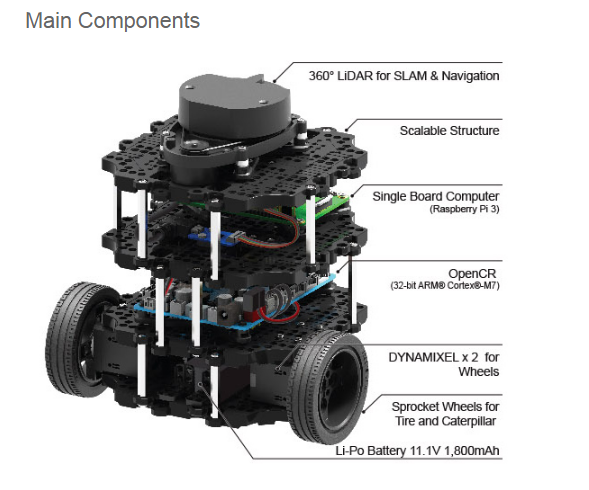
\includegraphics[width=7cm]{img/2_Theory/turtlebot3_burger.png}
        \caption{TurtleBot3 Burger}
        \end{subfigure}%
        \begin{subfigure}{0.5\textwidth}
        \centering
        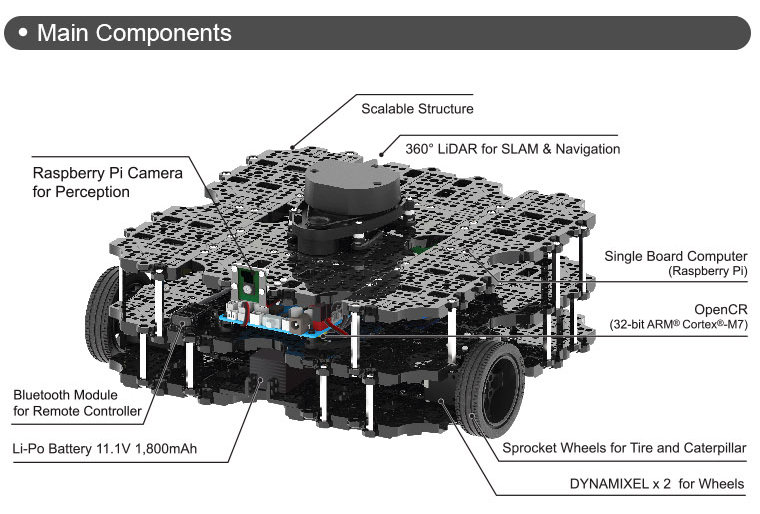
\includegraphics[width=7cm]{img/2_Theory/turtlebot3_waffle_pi.jpg}
        \caption{TurtleBot3 Waffle}
        \end{subfigure}
    \caption{Các dòng robot của TurtleBot3}
    \end{figure}
    \item \textit{Cảm biến}: Được trang bị với các cảm biến như cảm biến hồng ngoại, bộ cảm biến IMU (Inertial Measurement Unit), và camera, TurtleBot3 có khả năng thu thập dữ liệu môi trường và chính xác hóa động tác.
    \item \textit{Môi trường mô phỏng Gazebo:} TurtleBot3 được tích hợp chặt chẽ với Gazebo, một môi trường mô phỏng 3D, giúp người dùng kiểm thử và phát triển ứng dụng trong môi trường an toàn trước khi triển khai trên robot thực tế.
    \item \textit{Hỗ trợ học máy và trí tuệ nhân tạo:} Với tích hợp chặt chẽ với ROS, TurtleBot3 có thể được sử dụng để triển khai các thuật toán và mô hình học máy, từ điều hướng tự động đến nhận diện vật thể.
    \item \textit{Cộng đồng lớn và nguồn mở:} TurtleBot3 là một dự án nguồn mở với sự đóng góp từ cộng đồng lớn, tạo điều kiện cho việc chia sẻ kiến thức và phát triển cộng đồng người dùng.
\end{enumerate}
\subsection{Bài toán và ứng dụng đặt ra cho TurtleBot3}
\begin{itemize}
    \item \textit{Bài toán tránh vật cản:} Robot phải có khả năng phát hiện và tránh các vật cản trên đường đi của nó, bằng cách sử dụng các cảm biến và thuật toán học sâu.
    \item \textit{Bài toán điều hướng:} Robot phải có khả năng xác định vị trí của mình trong môi trường, bằng cách sử dụng các phương pháp như SLAM (Simultaneous Localization and Mapping) hoặc GPS (Global Positioning System).
    \item \textit{Bài toán giao tiếp:} Robot phải có khả năng giao tiếp với con người hoặc các robot khác, bằng cách sử dụng các phương tiện như âm thanh, hình ảnh, cử chỉ hoặc mạng không dây.
    \item \textit{Bài toán hợp tác:} Robot phải có khả năng hợp tác với các robot khác để thực hiện một nhiệm vụ chung, bằng cách sử dụng các thuật toán phối hợp và phân công.
\end{itemize}
\subsection{TurtleBot và phần cứng đã trang bị}
\begin{itemize}
    \item \textit{Robot:} Để phù hợp với làn đường, nhóm đã chọn Turtlebot dạng Burger. Bởi Burger cho phép ta đặt camera ở góc nhìn cao hơn, giống với thực tế hơn
    \item \textit{Camera:} Để có tầm nhìn bao quát cả phần dưới robot, nhóm đã trang bị camera với trường nhìn (FOV) là 160 độ
\end{itemize}
\section{ROS}
\subsection{ROS là gì?}
\begin{figure}[htp]
\begin{center}
    \includegraphics[width=7cm]{img/2_Theory/ROS.png}
    \caption{Logo ROS}
\end{center}
\end{figure}
\hspace{0.4cm}ROS\textsuperscript{\cite{ros}}, viết tắt của "Robot Operating System" (Hệ điều hành Robot), là một framework mã nguồn mở được thiết kế để hỗ trợ việc phát triển phần mềm cho robot. ROS không phải là hệ điều hành robot như tên gọi có thể khiến người ta hiểu lầm, mà nó là một tập hợp các công cụ, thư viện, và quy tắc chuẩn hóa giúp đơn giản hóa quá trình phát triển và chia sẻ phần mềm giữa các dự án robot.\\
\tab ROS được phát triển chủ yếu bởi Willow Garage và hiện nay được duy trì và phát triển bởi Open Robotics. Nó cung cấp một loạt các tính năng như quản lý thiết bị phần cứng, truyền thông giữa các module, quản lý gói phần mềm, và nhiều công cụ hỗ trợ khác để giúp nhà phát triển robot xây dựng và kiểm thử phần mềm của họ một cách dễ dàng.\\
\tab ROS là một hệ thống phần mềm phổ biến trong cộng đồng nghiên cứu và phát triển robot, được sử dụng rộng rãi trong các dự án về robot tự hành, robot công nghiệp, và nhiều ứng dụng khác liên quan đến lĩnh vực robotics.
\subsection{Ưu điểm của ROS}
\begin{enumerate}
    \item \textit{Mã nguồn mở, hoàn toàn miễn phí:} ROS là một dự án mã nguồn mở, điều này có nghĩa là người dùng có thể truy cập hoàn toàn miễn phí và sửa đổi mã nguồn theo nhu cầu.
    \item \textit{Tính linh hoạt:} ROS hỗ trợ nhiều ngôn ngữ lập trình như C++, Python,... giúp người phát triển lựa chọn ngôn ngữ phù hợp với kỹ năng và yêu cầu của dự án. (Source code của nhóm sử dụng ngôn ngữ Python để lập trình.)
    \item \textit{Thư viện và công cụ mạnh mẽ:}
    \begin{itemize}
        \item ROS cung cấp nhiều thư viện và công cụ hỗ trợ như thư viện điều khiển robot, thư viện thị giác máy tính, công cụ giả lập, và nhiều công cụ khác.
        \item Gazebo, một môi trường mô phỏng tích hợp sâu với ROS, giúp người phát triển kiểm thử và mô phỏng robot một cách hiệu quả.
    \end{itemize}
\end{enumerate}
\subsection{Phiên bản sử dụng}
\tab Hiện nay có khá nhiều phiên bản ROS như là ROS Kinetic, ROS Melodic, ROS Dashing,... Đối với đồ án này, nhóm quyết định sử dụng ROS Noetic. ROS Noetic là phiên bản thứ 13 của ROS. Nó được phát hành vào ngày 23 tháng 5 năm 2020. ROS Noetic chủ yếu hướng tới Ubuntu 20.04 (Focal), mặc dù các hệ thống khác được hỗ trợ ở các mức độ khác nhau.
\subsection{Các topic sử dụng}
\subsubsection{camera/image/compressed}
\subsubsection{cmd\_vel}
Ngoài các topic có sẵn của turtlebot ra, nhóm còn tạo các topic minh hoạ dữ liệu của các module để thuận tiện trong quá trình sửa lỗi.
\section{Gazebo}
\subsection{Gazebo là gì?}
\begin{figure}[h]
\begin{center}

\includegraphics[width=8cm]{img/2_Theory/gazebo.png}
\caption{Logo Gazebo}
\end{center}
\end{figure}
\hspace{0.4cm}Gazebo\textsuperscript{\cite{gazebo}} là một môi trường mô phỏng 3D mã nguồn mở được sử dụng chủ yếu trong lĩnh vực nghiên cứu và phát triển robot. Nó cung cấp một không gian ảo cho việc thử nghiệm, kiểm thử, và phát triển ứng dụng robot mà không cần phải triển khai trên robot thực tế.
\subsection{Đặc điểm}
\begin{enumerate}
    \item \textit{Mô phỏng chính xác:} Gazebo cung cấp một môi trường mô phỏng chính xác với độ chi tiết cao, giúp người phát triển kiểm thử và đánh giá hiệu suất của ứng dụng robot mà không cần phải thực hiện trên thiết bị thực tế.
    \item \textit{Đa nền tảng:} Hỗ trợ trên nhiều hệ điều hành như Linux, macOS, và Windows.
    \item \textit{Hỗ trợ công nghệ ROS:} Gazebo tích hợp chặt chẽ với ROS, giúp dễ dàng tích hợp và kiểm thử các ứng dụng ROS trong môi trường mô phỏng.
    \item \textit{Tích hợp với công cụ phát triển:} Gazebo tích hợp với các công cụ phát triển như RViz\textsuperscript{\cite{rviz}} và RQT, tạo ra một môi trường phát triển toàn diện cho robot.
    \item \textit{GUI (Graphical User Interface):} Gazebo cung cấp GUI thân thiện, dễ sử dụng với người dùng, thông qua các thanh menu, giúp người dùng tương tác trực tiếp trên gazebo mà không cần thông qua chỉnh sửa tệp mã.
\end{enumerate}
\subsection{Phiên bản sử dụng}
\tab Như đã giới thiệu ở phần \textbf{Đặc điểm}, Gazebo được tích hợp chặt chẽ với ROS, và ROS lại tương thích tốt với Ubuntu, nên nhóm đã cài đặt và sử dụng Gazebo phiên bản 11.11.0 trên Ubuntu để tiện cho việc mô phỏng.
\subsection{Mô tả robot}
\tab Để mô phỏng robot trong Gazebo, ta cần mô tả nó trong trong một file URDF (Unified Robot Description Format). URDF về cơ bản là một tệp XML cho phép mô tả các thuộc tính vật lý quan trọng của rô-bốt chẳng hạn như link (liên kết), joint (khớp nối), hình dạng, màu sắc, collision (va chạm), v.v. Trong đó tất cả các thành phần (liên kết và khớp nối) được định nghĩa bằng cách sử dụng tag.  Phiên bản URDF của Turtlebot3 Burger được nhóm lấy từ package Turtlebot3 Autorace 2020\textsuperscript{\cite{autorace}}.
\begin{figure}[!htb]
\begin{center}
    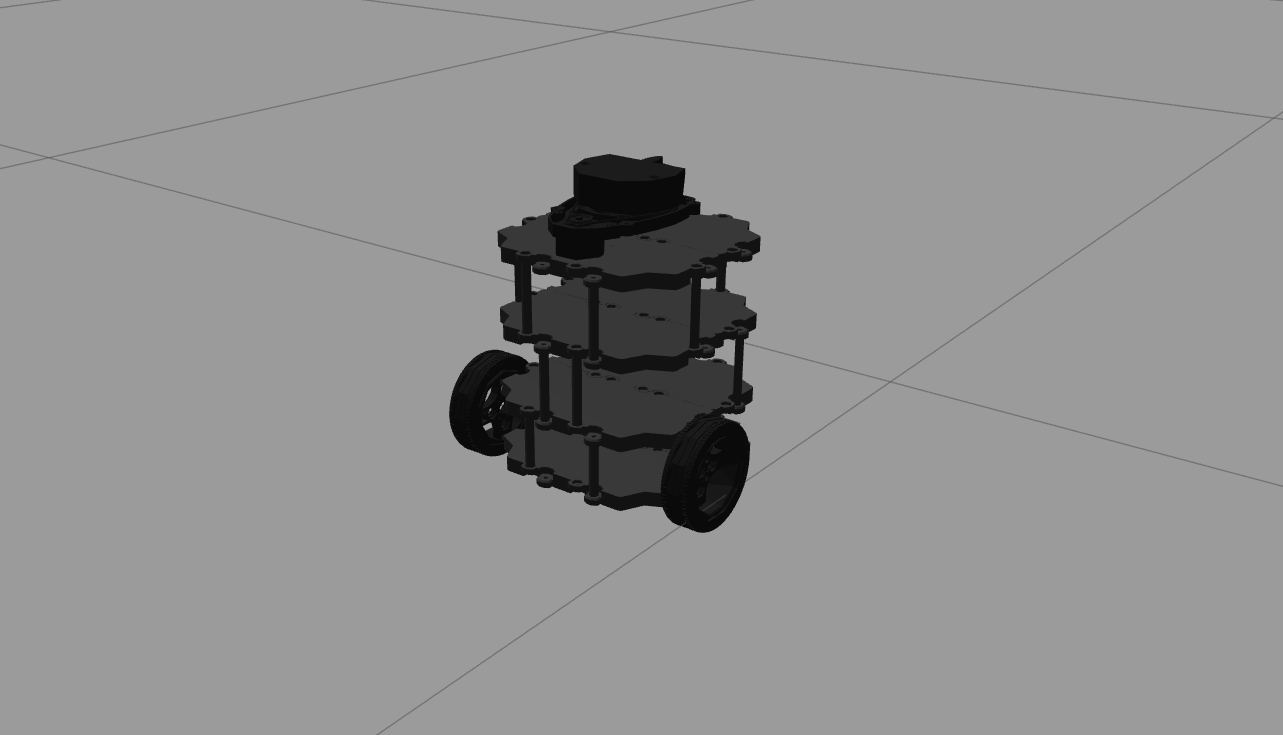
\includegraphics[width=12cm]{img/2_Theory/turtlebot3_burger_gazebo.png}
    \caption{Turtlebot3 Burger trong Gazebo}
\end{center}
\end{figure}
\subsection{Model làn đường}
\tab Gazebo sử dụng SDF (Simulation Description Format) để mô tả các yếu tố khác nhau của vật thể như robot, cảm biến, đèn, và các đối tượng môi trường như đất, tường, hoặc các vật thể khác. Nó giúp xác định vị trí, hình dạng, và các thuộc tính khác của các phần tử trong môi trường 3D.\\
\tab Phần mềm mà nhóm sử dụng để thiết kế model trong Gazebo là Blender\textsuperscript{\cite{blender}}. Blender là một phần mềm đồ họa 3D mã nguồn mở, mạnh mẽ và linh hoạt, phục vụ nhu cầu của nhiều lĩnh vực như đồ họa máy tính, nghệ thuật số, mô phỏng, và phát triển trò chơi.
\begin{figure}[!htb]
\begin{center}
    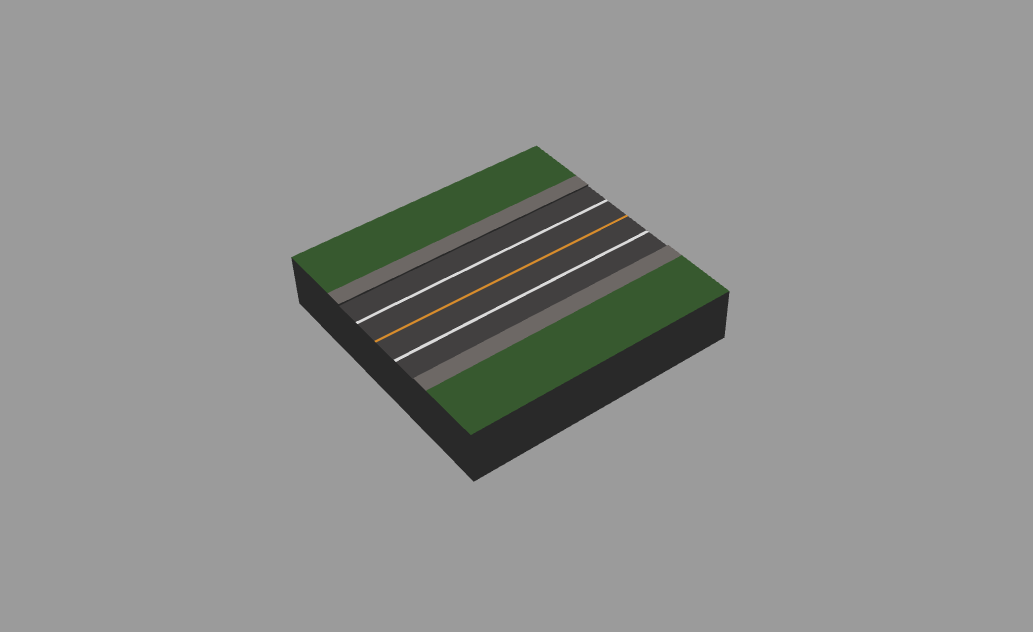
\includegraphics[width=12cm]{img/2_Theory/lane_model.png}
    \caption{Một phần làn đường trong Gazebo}
\end{center}
\end{figure}
\newpage
\section{Unity}
Ngoài công cụ mô phỏng Gazebo ra, nhóm còn sử dụng Unity để tạo dữ liệu cho việc huấn luyện model. Unity là Game Engine
\newpage
\section{OpenCV}
\subsection{OpenCV là gì?}
\begin{figure}[!hbt]
\begin{center}
    
\includegraphics[width=4cm]{img/2_Theory/opencv.png}
    \caption{Logo OpenCV}
\end{center}
\end{figure}
\tab OpenCV\textsuperscript{\cite{opencv}}, hay Open Source Computer Vision Library, là một thư viện mã nguồn mở chuyên về thị giác máy tính và xử lý ảnh. OpenCV được thiết kế để cung cấp một loạt các công cụ và thuật toán tiện ích để xử lý ảnh và video. Đồng thời, nó cũng được thiết kế để hỗ trợ hiệu quả về tính toán và chuyên dùng cho các ứng dụng thời gian thực. OpenCV có các giao diện cho ngôn ngữ lập trình C++, C, Python và Java và hỗ trợ các hệ điều hành như Windows, Linux, Mac OS, iOS và Android. 
\subsection{Ứng dụng}
\tab OpenCV được sử dụng cho đa dạng nhiều mục đích và ứng dụng khác nhau bao gồm: 
\begin{itemize}
    \item Hình ảnh street view.
    \item Kiểm tra và giám sát tự động.
    \item Robot và xe hơi tự lái.
    \item Phân tích hình ảnh y học.
    \item Tìm kiếm và phục hồi hình ảnh/video.
    \item Phim – cấu trúc 3D từ chuyển động.
    \item Nghệ thuật sắp đặt tương tác.
\end{itemize}
\subsection{Tính năng}
\begin{enumerate}
    \item \textit{Xử lý ảnh và video:} OpenCV cung cấp các thuật toán và công cụ để xử lý ảnh và video, bao gồm lọc ảnh, biến đổi hình thái, phát hiện cạnh, và nhiều công cụ khác.
    \item \textit{Thị giác máy tính:} Thư viện này hỗ trợ nhiều thuật toán thị giác máy tính, bao gồm nhận diện khuôn mặt, nhận diện đối tượng, theo dõi đối tượng, và nhận diện ký tự.
    \item \textit{Machine learning:} OpenCV tích hợp với các thư viện máy học như TensorFlow và PyTorch để thực hiện các nhiệm vụ như học máy và học sâu.
    \item \textit{Xử lý ảnh y tế: }OpenCV được sử dụng trong lĩnh vực y tế để phân tích hình ảnh y khoa và hỗ trợ các ứng dụng như dự đoán bệnh, phân loại tế bào, và nhiều công việc khác.
    \item \textit{Robotics:} OpenCV được tích hợp trong nhiều dự án robotics để xử lý ảnh từ các camera và cảm biến.
    \item \textit{Real-time Computer Vision:} OpenCV hỗ trợ thị giác máy tính thời gian thực, làm cho nó phù hợp cho ứng dụng như xe tự lái, video giám sát, và robot di động.
\end{enumerate}
\subsection{Chọn ngôn ngữ nào để lập trình OpenCV?}
\tab OpenCV hiện tại hỗ trợ nhiều ngôn ngữ, mỗi ngôn ngữ có thế mạnh riêng, vậy thì tùy theo nhu cầu mà chọn ngôn ngữ cho phù hợp.
\begin{itemize}
    \item \textit{C++:} Đây là ngôn ngữ phổ biến nhất hiện tại vì nhanh, có nhiều lựa chọn.
    \item \textit{Python:} Ngôn ngữ được dùng nhiều để thử nghiệm/kiểm tra OpenCV do tính ngắn gọn, ít phải thiết lập. Bên cạnh đó, nếu dùng Python thì cũng có thể code được trên nhiều hệ điều hành.
    \item \textit{Java:} Nhanh và đa nền tảng, tương tự C++.
\end{itemize}
\tab Đối với đề tài, nhóm sử dụng ngôn ngữ Python để lập trình.
\section{Thuật toán Hough Line Transform}
\subsection{Phương trình đường thẳng trong không gian ảnh}
\tab Ở cấp bậc trung học, chúng ta đã biết phương trình đường thẳng cơ bản được biểu diễn bởi 2 tham số $a$ và $b$ như sau:
\begin{center}
$y = ax + b$    
\end{center}
\begin{figure}[htp]
\begin{center}
    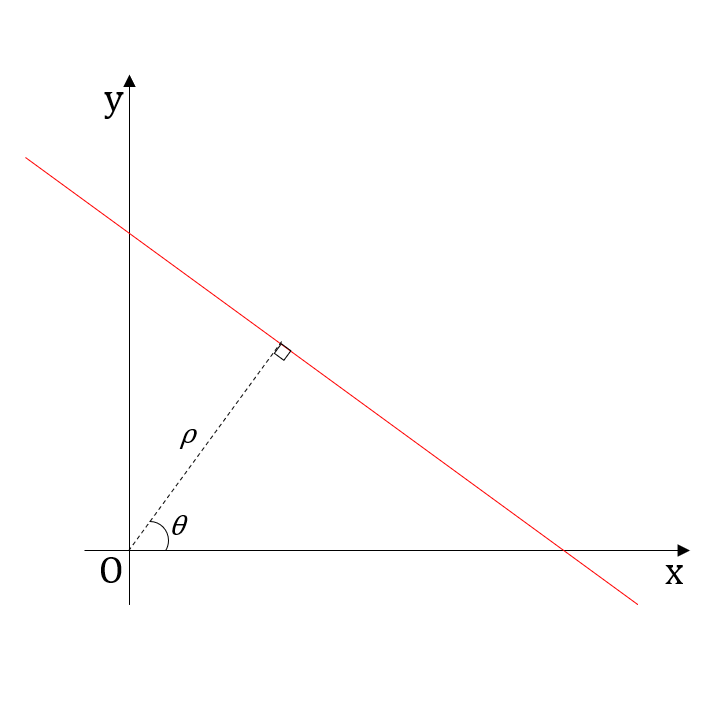
\includegraphics[width=8cm]{img/2_Theory/hough_trans_1.png}
    \caption{Phương trình đường thẳng $y = ax + b$ trong không gian ảnh}
\end{center}
\end{figure}
\tab Tuy nhiên, với cách biểu diễn này, giá trị của hệ số chặn $a$ trải dài từ $-\infty$ đến $+\infty$. Có thể lấy ví dụ, để có được phương trình đường Oy $(x = 0)$ thì $a$ phải tiến tới $\infty$. Thuật toán Hough  Line Transform\textsuperscript{\cite{houghtransform}} yêu cầu các giá trị $a$, $b$ nằm trong một khoảng xác định (hay bị chặn trên dưới), ta phải sử dụng hệ tọa độ cực để biểu diễn phương trình đường thẳng. Cách biểu diễn này cũng nằm trong chương trình toán trung học:
\begin{center}
$\rho = xcos(\theta) + ysin(\theta)$    
\end{center}
với $\rho$ là khoảng cách vuông góc từ gốc tọa độ O tới đường thẳng và $\theta$ là góc hợp bởi đường thẳng vuông góc này với trục hoành, được tính theo ngược chiều kim đồng hồ.\\
\tab Xét thấy trong phương trình tọa độ cực, giá trị của góc $\theta$ có thể bị chặn lại trong khoảng $[0, \pi)$. Trên thực tế, không gian ảnh là không gian hữu hạn (bị chặn lại bởi các cạnh của ảnh), do vậy giá trị $\rho$ cũng bị chặn.
\subsection{Ánh xạ giữa không gian ảnh và không gian Hough}
\tab Từ một đường thẳng trong không gian ảnh với 2 tham số là $\rho$ và $\theta$, ta sẽ ánh xạ sang không gian Hough thành 1 điểm.
\begin{figure}[htp]
\begin{center}
    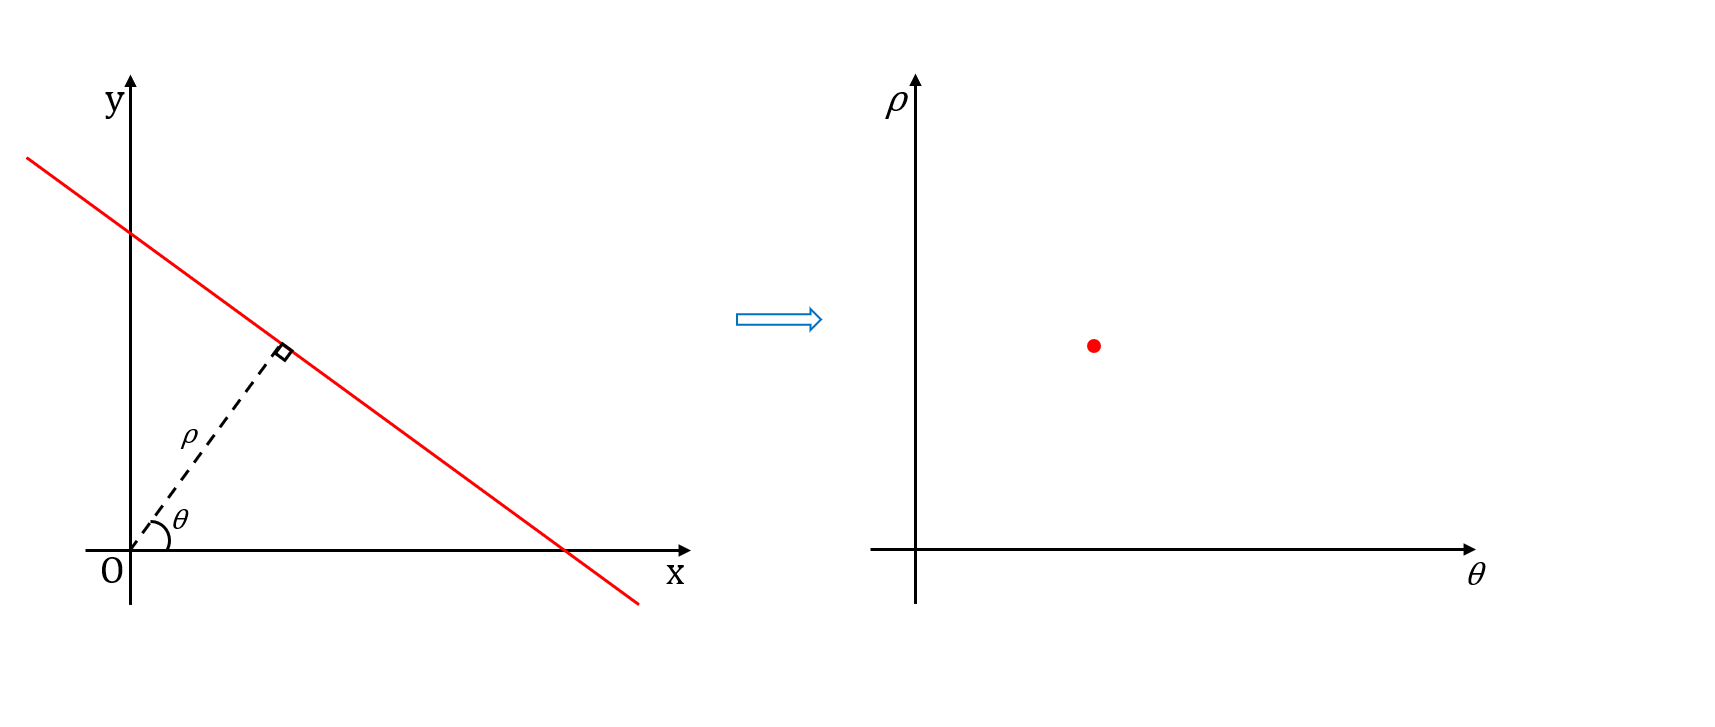
\includegraphics[width=13cm]{img/2_Theory/hough_trans_3.jpg.png}
    \caption{\centering Ánh xạ một đường thẳng từ không gian ảnh thành một điểm trong không gian Hough}
\end{center}
\end{figure}
\newpage
\tab Còn từ một điểm trong không gian ảnh, có tọa độ $(x, y)$, ta thu được một hình sin trong không gian Hough.\\
\begin{figure}[!htp]
\begin{center}
    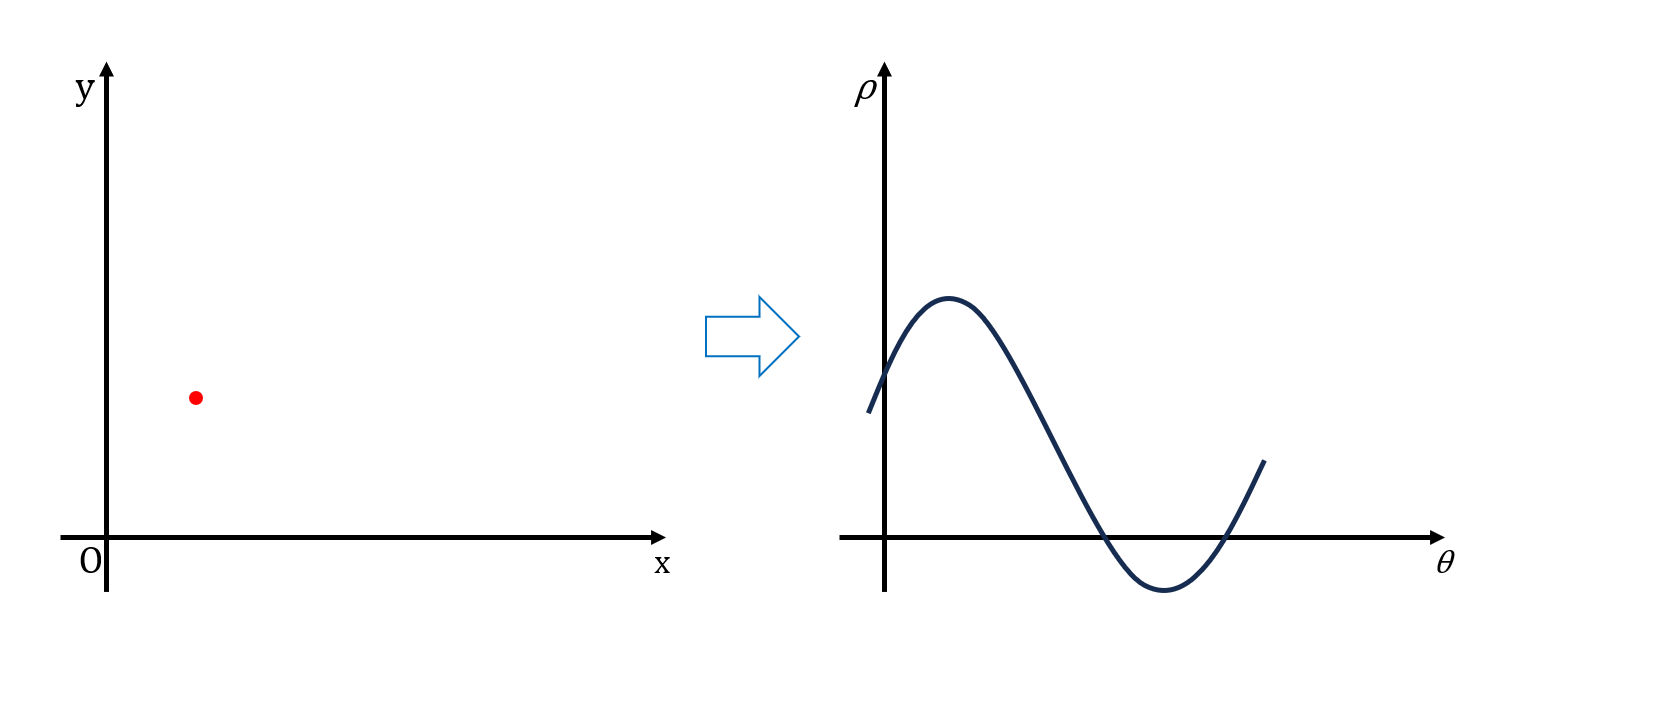
\includegraphics[width=12cm]{img/2_Theory/hough_trans_4.jpg.png}
    \caption{\centering Ánh xạ một điểm từ không gian ảnh thành một hình sin trong không gian Hough}
\end{center}
\end{figure}
\\
\tab Các điểm nằm trên cùng một đường thẳng sẽ biểu diễn được các hình sin giao nhau tại một điểm trong không gian Hough. Dựa vào ý tưởng này, thuật toán Hough Line Transform sẽ chọn được phương trình đường thẳng đi qua nhiều điểm nhất thông qua việc bình chọn. Tuy nhiên, trong thực tế, trong một bức ảnh thường có nhiều hơn một cạnh, như vậy, việc lấy đường thẳng có số pixel đi qua nhiều nhất sẽ không phù hợp. Thay vào đó, chúng ta sẽ đặt ra một ngưỡng số lượng pixel nhất định, nếu trên ngưỡng này thì được xem là đường thẳng và ngược lại.
\begin{figure}[htp]
\begin{center}
    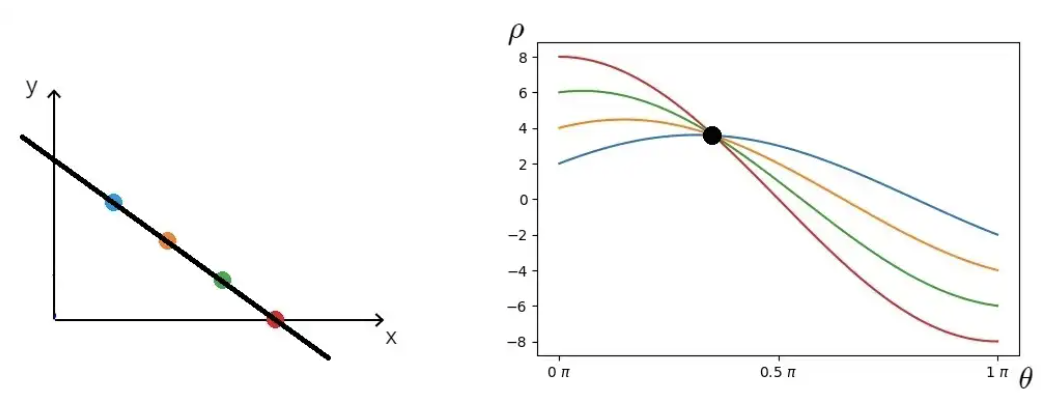
\includegraphics[width=14cm]{img/2_Theory/hough_trans_5.png}
    \caption{\centering Hình ảnh minh họa cho ánh xạ nhiều điểm trên đường thẳng trong không gian ảnh sang không gian Hough}
\end{center}
\end{figure}
\subsection{Hough Line Transform hoạt động như thế nào?}
\subsubsection{Tiền xử lý}
\tab Để thu được các đường thẳng như mong muốn, ảnh cần được xử lý trước khi thực hiện thuật toán Hough Line Transform. Hough Line Transform yêu cầu đầu vào là một ảnh nhị phân. Trên thực tế ảnh sẽ được đưa về dạng ảnh xám, áp dụng các thuật toán lọc biên để xác định các đường biên trong ảnh. Ở đây chúng ta sẽ sử dụng thuật toán Canny để lọc biên. \\
\tab Đối với đề tài của nhóm, đầu vào của thuật toán Hough Line Transform là một ảnh dạng nhị phân, do đó ta sẽ bỏ qua bước tiền xử lý này.
\subsubsection{Bình chọn đường thẳng}
\tab Ta chia không gian Hough thành các lưới ô vuông nhỏ. Ta thu được một lưới ô vuông (ma trận) với các hàng là trục $\rho$ và các cột là trục $\theta$ như hình \ref{accumlator}. Độ chính xác của thuật toán phụ thuộc vào số lượng các ô vuông ta chọn cho mỗi cạnh. Giả sử ta muốn độ chính xác của $\theta$ là $1^{\circ}$, ta cần 180 cột. Giá trị $\rho$ bị chặn bởi cạnh chéo của ảnh đầu vào. Do vậy khi lấy độ chính xác của $\rho$ là 1 (pixel) thì số hàng bằng độ dài đường chéo ảnh theo đơn vị pixel.\\
\begin{figure}[ht]
\begin{center}
    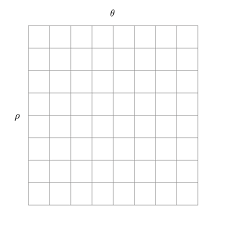
\includegraphics[width=6cm]{img/2_Theory/hough_trans_2.png}
    \caption{Lưới ô vuông (ma trận) minh họa thu được từ không gian Hough}
    \label{accumlator}
\end{center}
\end{figure}
\newpage
\tab Giá trị tại mỗi ô ban đầu trong ma trận được đặt bằng 0. Xét các điểm trên ảnh đầu vào (chính là ảnh nhị phân thu được sau bước tiền xử lý), với mỗi điểm sáng, ta xét $\theta$ trong khoảng $[0, 180)$. Vì đã biết tọa độ điểm $(x, y)$, ta dễ dàng tính được giá trị $\rho$. Với mỗi cặp ($\rho, \theta$), ta thực hiện bình chọn (tăng giá trị ô tương ứng trong ma trận lên 1 đơn vị). Cuối cùng ta thực hiện lấy ngưỡng để xác định trên lưới ô vuông đường thẳng nào ứng với một đường thẳng trên thực tế.
\section{K-means Clustering}
\section{Curve fitting}
\section{Image Segmentation}
\subsection{Image Segmentation là gì}
\tab Image Segmentation (phân đoạn ảnh) là một phần quan trọng trong lĩnh vực Computer Vision (thị giác máy tính). Nó là quá trình chia nhỏ một bức ảnh thành nhiều phần, với mục tiêu đơn giản hóa hoặc thay đổi biểu diễn của bức ảnh để dễ dàng phân tích. Image Segmentation cũng có một mục tiêu chung với Object Detection (phát hiện vật thể) là phát hiện ra vùng ảnh chứa vật thể và gán nhãn phù hợp cho chúng. Tuy nhiên tiêu chuẩn về độ chính xác của Image Segmentation ở mức cao hơn so với Object Detection khi nó yêu cầu nhãn dự báo đúng tới từng pixel.\\
\tab Trong quá trình này, mỗi pixel trong hình ảnh được liên kết với một loại đối tượng. Có hai kiểu Image Segmentation là Semantic Segmentation và Instance Segmentation. Từ đó, Image Segmentation có thể chỉ ra thông tin chi tiết của bức ảnh, bao gồm: Vị trí của vật thể trong ảnh, hình dạng của vật thể và từng pixel nào thuộc về vật thể nào.
\begin{figure}[htp]
\begin{center}
    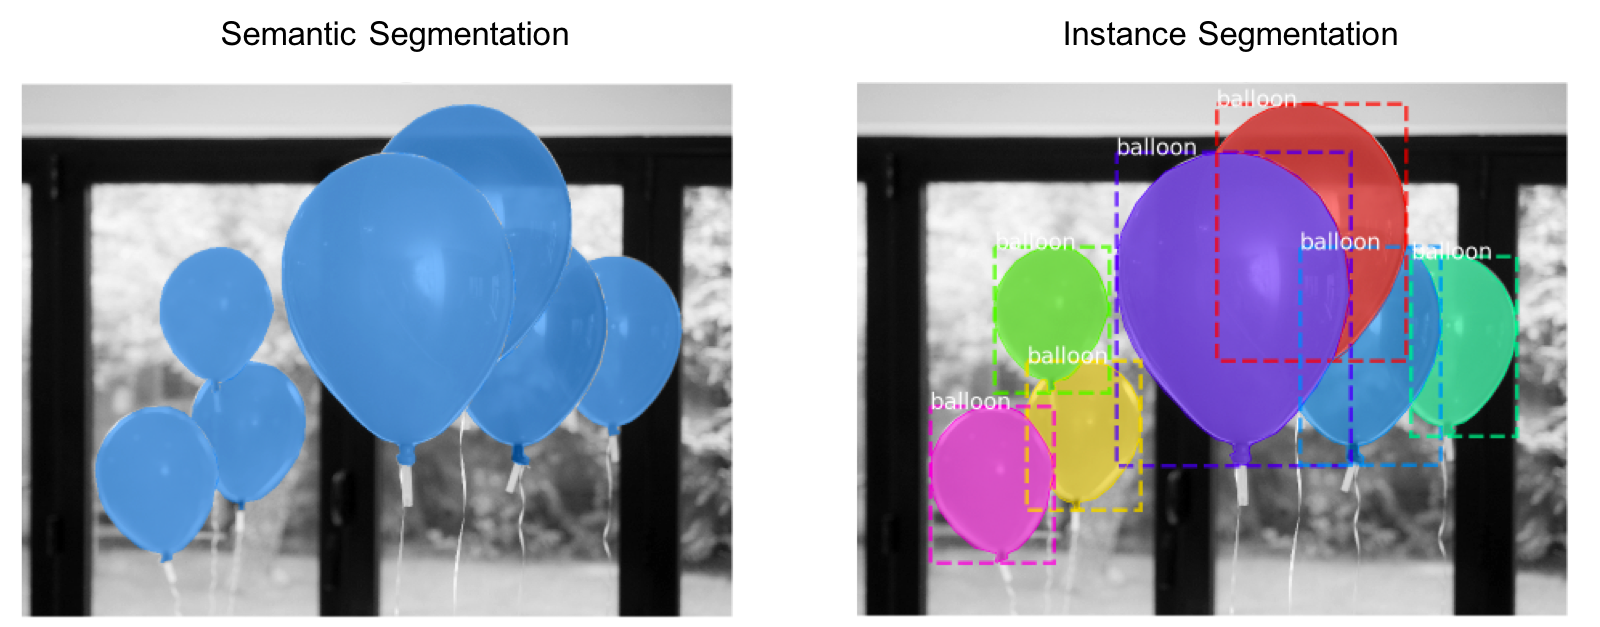
\includegraphics[width=15cm]{img/2_Theory/ss-is.png}
    \caption{Semantic Segmentation và Instance Segmentation}  
\end{center}
\end{figure}
\subsection{Kiến trúc hệ thống Image Segmentation}
\tab Kiến trúc cơ bản trong Image Segmentation bao gồm một bộ encoder (mã hoá) và decoder (giải mã).\\
\begin{figure}[!htb]
\begin{center}
    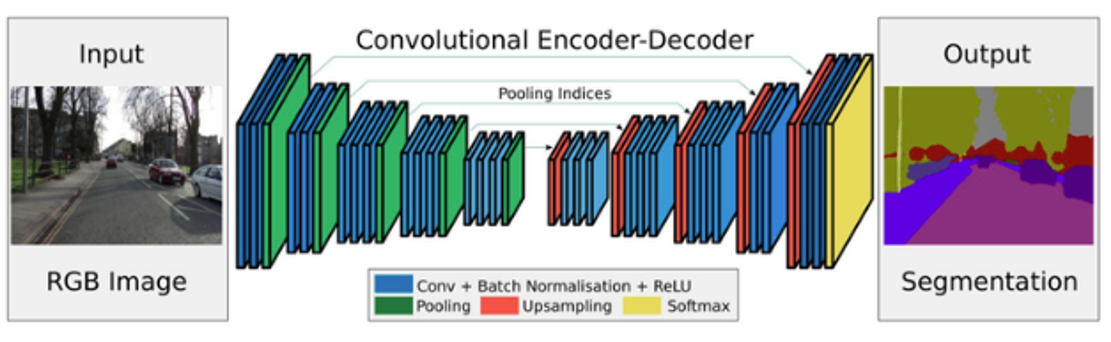
\includegraphics[width=15cm]{img/2_Theory/conv-encode-decode.png}
    \caption{Kiến trúc Convolutional Encoder-Decoder}  
\end{center}
\end{figure}\\
\tab Encoder trích xuất các tính năng từ hình ảnh thông qua các bộ lọc. Decoder chịu trách nhiệm tạo ra đầu ra cuối cùng thường là một mặt nạ phân đoạn chứa đường viền của đối tượng.
\subsection{Ứng dụng}
\tab Phân vùng ảnh có rất nhiều các ứng dụng trong y học, xe tự hành, xử lý ảnh vệ tinh, ...
\begin{itemize}
\item Y học: Trong y học, thuật toán Image Segmentation có thể hỗ trợ bác sĩ chẩn đoán khối u từ ảnh x-quang. Ưu điểm của Image Segmentation đó là không chỉ cho chúng ta biết vị trí của các khối u trong ảnh mà còn cho chúng ta biết được hình dạng của chúng.
\item Xe tự hành: Xe tự hành đòi hỏi phải liên tục nhận thức, xử lý và lên kế hoạch trong một môi trường luôn có sự thay đổi. Vì yêu cầu an toàn tuyệt đối và độ chính xác cao trong mọi quyết định nên một hệ thống xe tự hành cần phải xác định chính xác các vật thể xuất hiện khi tham gia giao thông như người, đèn tín hiệu, biển báo, vạch kẻ đường, xe cộ.
\item Xử lý ảnh vệ tinh: Các vệ tinh quay quanh trái đất sẽ liên tục thu thập hình ảnh bề mặt trái đất ở những vùng khác nhau. Từ các bức ảnh chụp vệ tinh, mô hình Image Segmentation sẽ phân đoạn hình ảnh thành tuyến đường, khu phố, biển cả, cây cối,….
\item Ứng dụng trong nông nghiệp: Chúng ta có thể tiết kiệm được một lượng lớn thuốc trừ sâu trong nông nghiệp nhờ sử dụng hệ thống phun thuốc trừ sâu tự động có khả năng phân biệt được diện tích cỏ và cây trồng dựa trên thuật toán Image Segmentation. Khi diện tích cỏ lấn át so với cây trồng thì hệ thống sẽ tự động kích hoạt.
\item Cảnh báo cháy rừng: Những hệ thống kiểm soát cháy rừng có thể segment được chính xác vị trí phát sinh các đám cháy từ ảnh chụp vệ tinh. Từ đó đưa ra cảnh báo về quy mô và mức độ lây lan của các đám cháy trên diện rộng.
\end{itemize}
\section{TwinLiteNet}
\tab Sau khi thực hiện nhiều thử nghiệm với các model khác nhau, nhóm đã quyết định sử dụng model TwinLiteNet\textsuperscript{\cite{twinlitenet}} cho đồ án. Khác biệt với các model nhận diện làn đường khác như UNet \textsuperscript{\cite{unet}}, LaneNet\textsuperscript{\cite{lanenet}}, YOLOPv2\textsuperscript{\cite{yolopv2}},... mà thường yêu cầu sử dụng nhiều tài nguyên và đòi hỏi phần cứng mạnh mẽ, TwinLiteNet được xây dựng như một model nhẹ (lightweight) nhưng vẫn đảm bảo độ chính xác và hiệu quả cao. Quyết định này nhằm tối ưu hiệu suất và độ nhẹ của model, giúp model có thể triển khai một cách linh hoạt trên các hệ thống có công suất tính toán hạn chế, như là những thiết bị nhúng trong xe tự hành.\\
\begin{figure}[h]
\begin{center}
    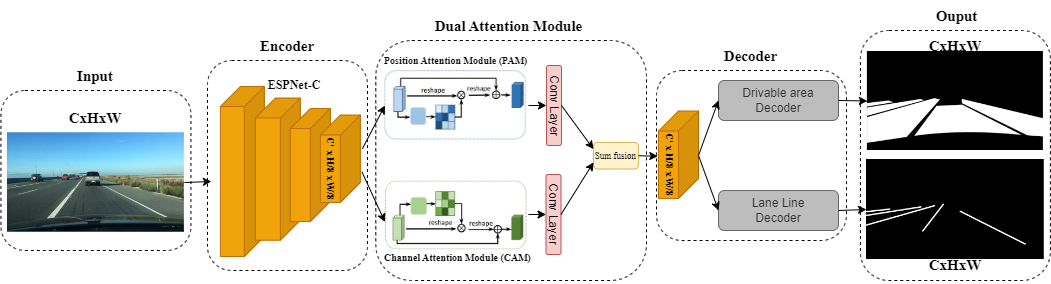
\includegraphics[width=16.5cm]{img/2_Theory/TwinLiteNet_arch.png}
    \caption{Kiến trúc TwinLiteNet}
\end{center}
\end{figure}\\
\tab TwinLiteNet sử dụng ESPNNet-C làm encoder để trích xuất các đặc trưng (feature) của ảnh gốc. Các đặc trưng được rút trích sẽ đi qua một bộ Dual Attention Module. Dual Attention Module bao gồm Position Attention Module (PAM) và Channel Attention Module (CAM). CAM tạo điều kiện thuận lợi cho việc tổng hợp thông tin đặc trưng của ảnh theo kênh, trong khi PAM được thiết kế để nắm bắt và tổng hợp các điểm ảnh (pixel) liên quan đến ngữ nghĩa trong miền không gian. Đầu ra của hai module sẽ được biến đổi bằng một lớp Convolutional và được tổng hợp lại bằng hàm cộng theo phần tử. Thay vì sử dụng một decoder duy nhất cho tất cả các loại đối tượng, thì TwinLiteNet sử dụng hai decoder để xử lý ma trận (map) đặc trưng và cho các tác vụ riêng biệt Drivable Area và Lane Segmentation
\subsection{Tập dữ liệu BDD100K}
\tab BDD100K\textsuperscript{\cite{bdd100k}} là tập dữ liệu hình ảnh dùng để huấn luyện các mô hình trí tuệ nhân tạo trong việc nhận dạng và phân loại hình ảnh. Tập dữ liệu này chứa hơn 100.000 hình ảnh và video được gắn nhãn, được thu thập từ các camera trên xe hơi. BDD100K được sử dụng rộng rãi trong các nghiên cứu về xe tự hành và các ứng dụng liên quan đến trí tuệ nhân tạo
\begin{figure}[!hbt]
\begin{center}
    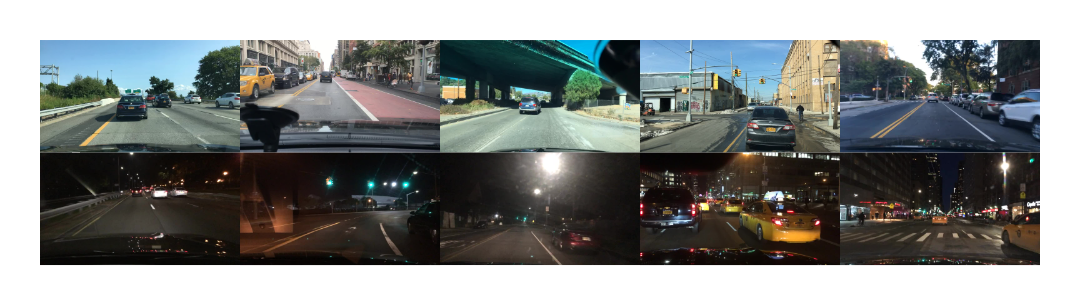
\includegraphics[width=16.5cm]{img/2_Theory/bdd100k.png}
    \caption{Minh hoạ tập dữ liệu BDD100K}
\end{center}
\end{figure}\\
\subsection{Hàm loss}
\tab Hai hàm loss được sử dụng trong model là Focal Loss\textsuperscript{\cite {focalloss}} và Tversky Loss\textsuperscript{\cite{tverskyloss}}. Focal Loss nhằm hạn chế sự ảnh hưởng của các mẫu dễ dự báo lên hàm loss và phạt nặng vào các mẫu khó dự báo, như ở phương trình. Ngược lại, Tversky Loss là một biến thể của Dice Loss, là độ đo để đánh giá kết quả segment. Khác với Dice Loss\textsuperscript{\cite{diceloss}}, Tversky Loss đánh thêm trọng số vào False Positives và False Negatives
\begin{equation}
Loss_{focal} = - \frac{1}{N}\sum_{C = 0}^{C - 1}\sum_{i = 1}^{N}p_i(c)(1 - \hat{p}_i(c))^{\gamma}log(\hat{p}_i(c))
\end{equation}
trong đó:
\begin{itemize}
    \item N: Số lượng pixel của ảnh
    \item C: Số lượng lớp, trong trường hợp này, một lớp là làn đường, và lớp còn lại là nền.
    \item \(\hat{p}_i(c)\): Xác định dự đoán cho pixel thứ 
i của lớp c
    \item \(p_i(c)\): Giá trị thực tế (ground truth) cho pixel thứ i của lớp c.
    \item \(\gamma\): Hệ số điều chỉnh cân bằng
\end{itemize}
\begin{equation}
Loss_{tversky} = - \frac{1}{N}(1 - \frac{TP(c)}{TP(c) - \alpha FN(c) \beta FP(c)})
\end{equation}
trong đó:
\begin{itemize}
    \item TP: True Positives
    \item FN: False Negatives
    \item FP: False Positives
    \item C: Số lượng lớp, trong trường hợp này, một lớp là làn đường, và lớp còn lại là nền.
    \item \(\alpha, \beta\): Điều khiển độ phạt cho FP và FN
\end{itemize}
Hàm loss tổng hợp sẽ có dạng:
\begin{equation}
Loss_{total} = Loss_{focal} + Loss_{tversky}
\end{equation}
\section{Bộ điều khiển PID}
\subsection{PID là gì}
\tab PID\textsuperscript{\cite{pid}} được viết tắt bởi cụm từ \textbf{Proportional Integral Derivative}, có nghĩa là 1 cơ chế phản hồi các vòng điều khiển, chúng được ứng dụng rộng rãi trong hệ thống điều khiển công nghiệp hiện đại.\\
\tab Bộ điều khiển này sử dụng nhiều trong những hệ thống điều khiển vòng kín có tín hiệu phản hồi. Nhiệm vụ của PID giúp tính toán giá trị sai số là hiệu số giữa giá trị đo thông số biến đổi với giá trị đặt mong muốn.\\
\begin{figure}[!hbt]
\begin{center}
    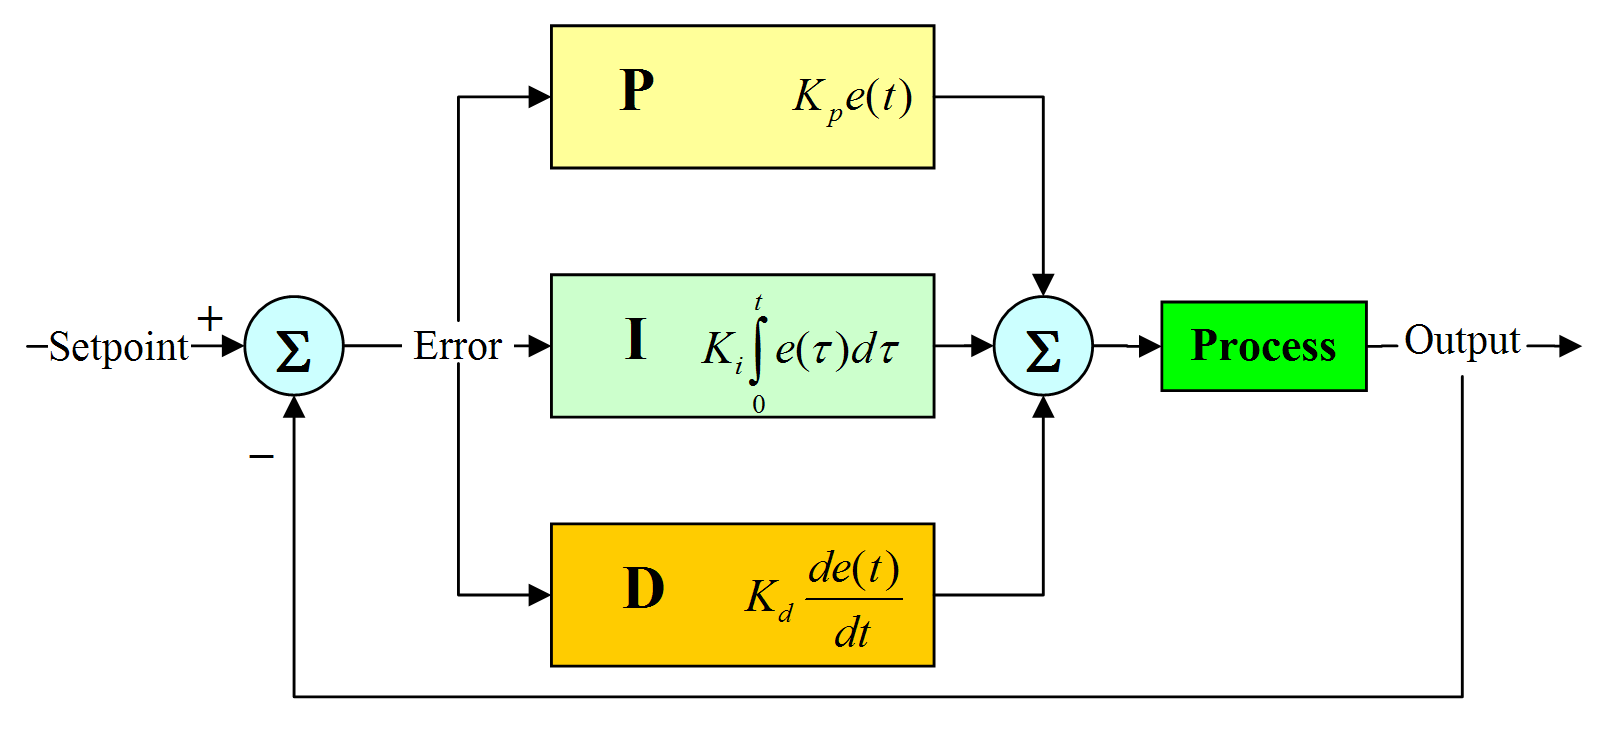
\includegraphics[width=14cm]{img/2_Theory/pid.png}
    \caption{Sơ đồ khối của hệ thống PID}
\end{center}
\end{figure}
\\
\tab Bộ thiết bị làm giảm tối đa sai số bằng cách điều chỉnh giá trị điều khiển đầu vào. Để đạt được hiệu quả mong muốn bởi thông số của PID cần phải thực hiện điều chỉnh theo tính chất hệ thống. Việc điều khiển sẽ giống nhau, còn thông số được phụ thuộc vào chính đặc thù của hệ thống đó.

\begin{itemize}
    \item P: là phương pháp điều chỉnh tỉ lệ, tạo ra tín hiệu điều chỉnh tỉ lệ với sai lệch đầu vào theo thời gian lấy mẫu.
    \item I: là tích phân của sai lệch theo thời gian lấy mẫu. Điều khiển tích phân là phương pháp điều chỉnh để tạo ra các tín hiệu điều chỉnh sao cho độ sai lệch giảm về 0. Từ đó cho biết tổng sai số tức thời theo thời gian hay sai số tích lũy trong quá khứ. Khi thời gian càng nhỏ thể hiện tác động điều chỉnh tích phân càng mạnh, tương ứng độ lệch càng nhỏ.
    \item D: là vi phân của sai lệch. Điều khiển vi phân tạo ra tín hiệu điều chỉnh sao cho tỉ lệ với tốc độ thay đổi sai lệch đầu vào. Thời gian càng lớn thì phạm vi điều chỉnh vi phân càng mạnh, tương ứng với bộ điều chỉnh đáp ứng với thay đổi đầu vào càng nhanh.
\end{itemize}
\subsection{Ứng dụng}
\tab Hiện nay PID được ứng dụng trong nhiều ngành nghề khác nhau:
\begin{itemize}
    \item Nó có thể được dùng để giảm các sai số, hạn chế sự dao động hay là giảm thời gian gian xác lập và độ vọt lố…
    \item Sử dụng để điều khiển mực nước: bộ điều khiển được tự động hóa nhờ vào các thiết bị điện tử như cảm biến, van điều khiển…
    \item Điều khiển biến tần: Các thiết bị điện tử kết hợp ở đây gồm có: van điều khiển lưu lượng, cảm biến nhiệt độ, biến tần điều khiển….
    \item Kiểm soát lưu lượng khí qua đường ống
\end{itemize}
\newpage
\chapter{Kiến trúc hệ thống}

Kiến trúc chung của hệ thống mà nhóm đưa ra sẽ có kiến trúc như sau:

\begin{figure}[htp]
    \centering
    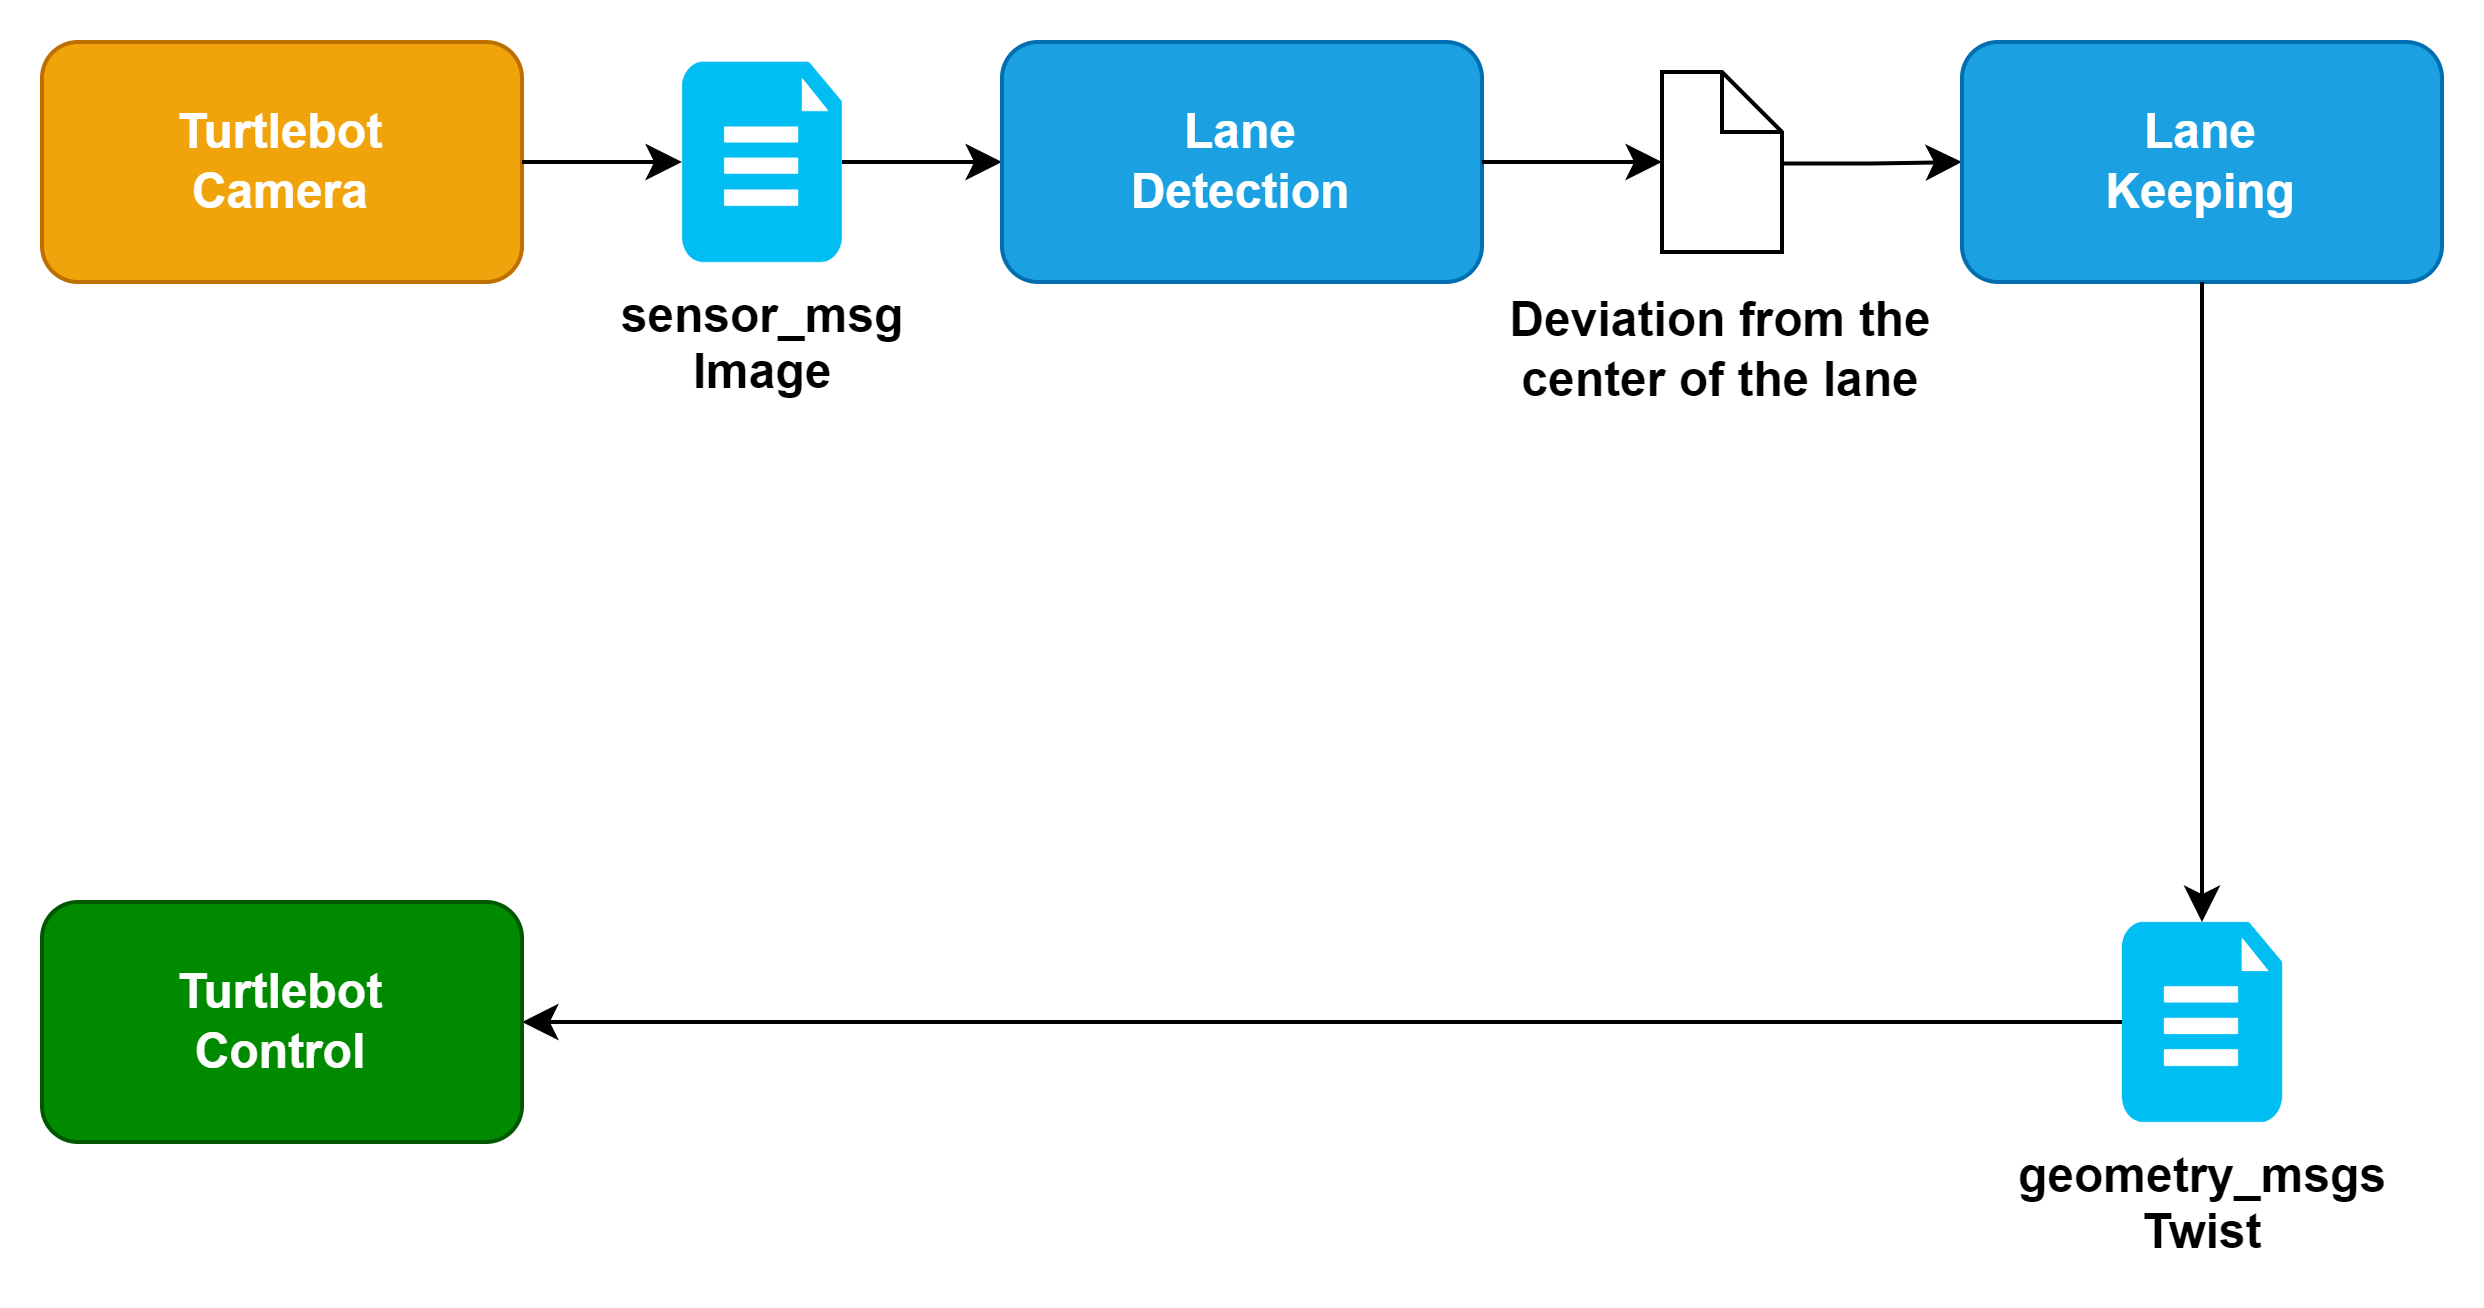
\includegraphics[width=\linewidth]{img/3_Architecture/general_arch.png}
    \captionof{figure}{Kiến trúc hệ thống}
\end{figure}

Trong đó các module hiện tại được hiện thực và có các chức năng sau:

\begin{itemize}
    \item \textbf{Module nhận diện làn đường:} Nhận đầu vào là ảnh trực tiếp từ camera, module sẽ xử lý và tìm hai phương trình làn đường \textbf{LL} (left\_lane), \textbf{RL}(right\_lane) đại diện cho hai làn đường và xác định độ lệch của robot so với tâm làn đường.
    \item \textbf{Module bám làn đường:} Đưa ra hành vi di chuyển của robot dựa vào kết quả thu thập được từ module phát hiện làn đường.
\end{itemize}

\section{Module nhận diện làn đường}

\subsection{Giới thiệu chức năng}

Module nhận diện làn đường là một trong những module nhận dữ liệu trực tiếp từ camera. Sau quá trình xử lý, module sẽ có được phương trình đường thẳng của hai làn đường được hai làn đường dự đoán và cung cấp thông tin cho hệ thống bám làn. Ngoài ra, Module nhận diện làn đường tương tác với Module bám làn đường để cung cấp thông tin vị trí của làn đường, ảnh hưởng đến quyết định lái xe.

\subsection{Mô tả chi tiết}
Module nhận diện làn đường như một hàm có tham số đầu vào và đầu ra như sau:
\begin{itemize}
    \item Input: Hình ảnh được trích xuất từ camera với kích cỡ 640 × 480 × 3
    \item Output: Độ lệch robot so với tâm làn đường.
\end{itemize}
Dữ liệu bên trong module sẽ đi qua các bước sau:
\newpage
\begin{figure}[!hbt]
    \centering
    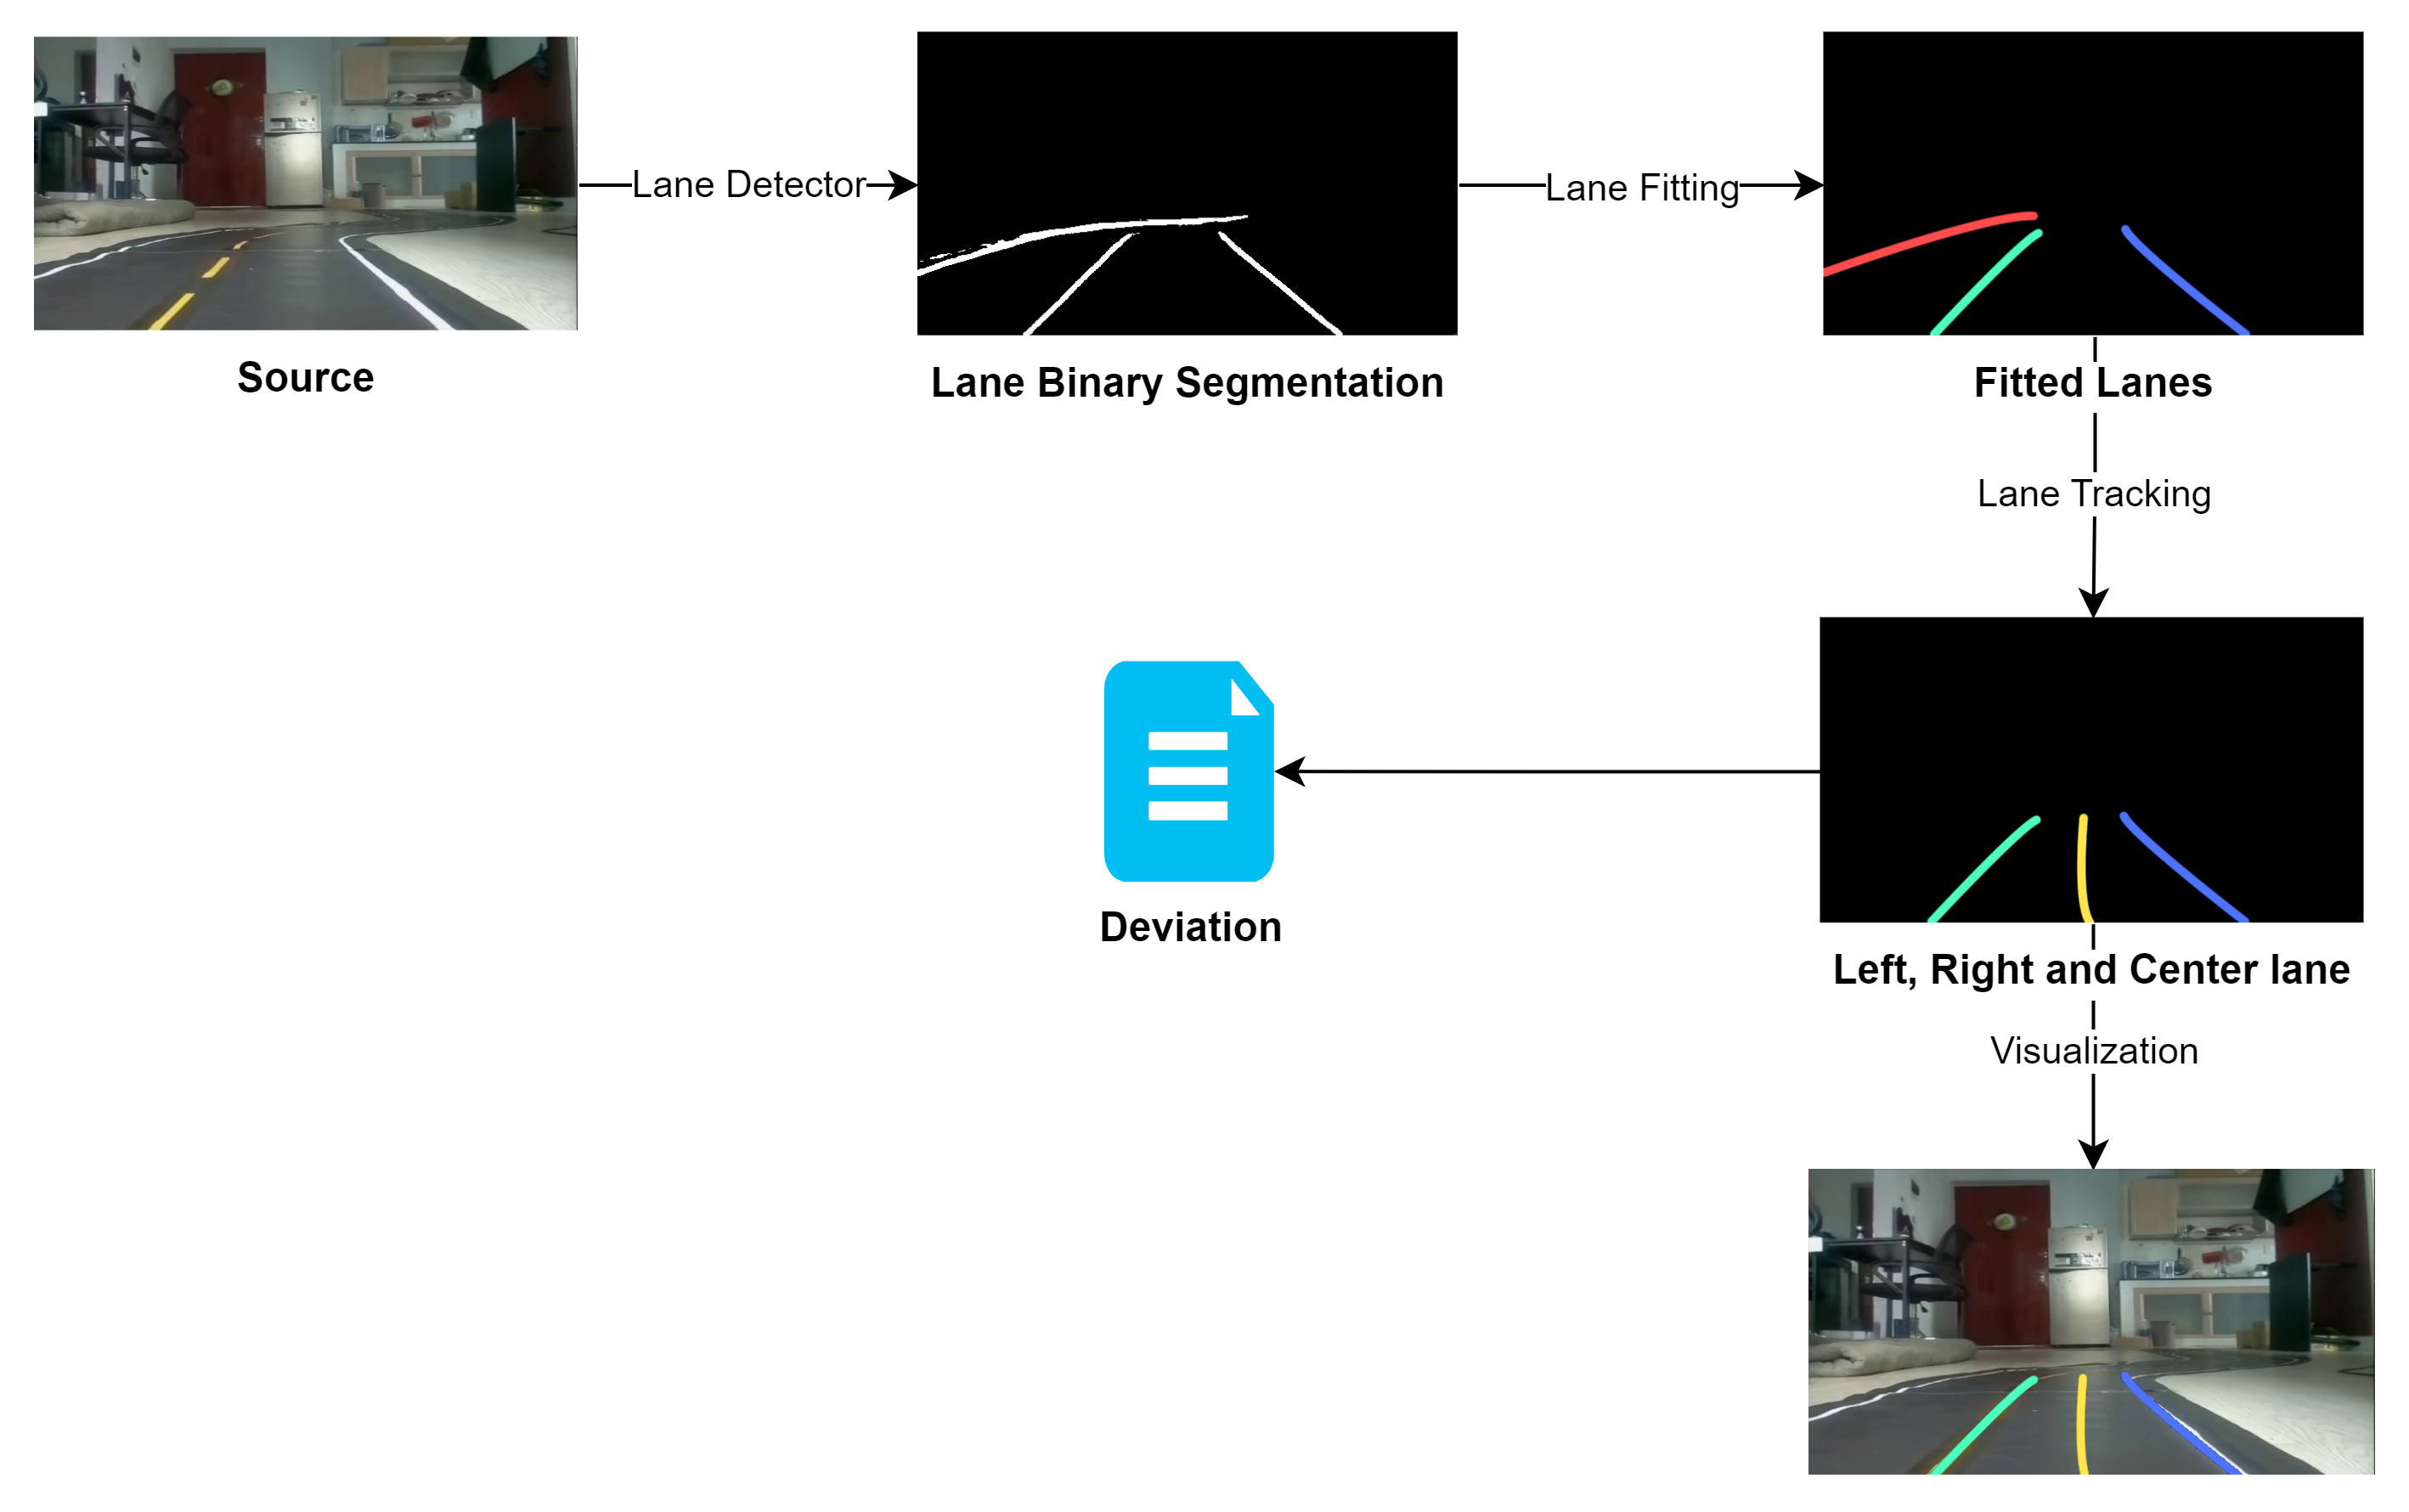
\includegraphics[width=15cm]{img/3_Architecture/lane_detector_arch.png}
    \captionof{figure}{Cấu trúc của module nhận diện làn đường}
\end{figure}

% TODO: Liệu có nên bỏ phần dưới đây

% \begin{itemize}
%     \item Model AI (khoảng 10ms với RTX4070 và CUDA 12.3): Segmentation những vùng có làn đường và trả về một bức ảnh dạng binary 640 x 360 x 1.
%     \item Backend: (khoảng 4ms): Sử dụng dữ liệu trả về bởi model, lọc những nhiễu và xử lý để cho ra phương trình đường thẳng hai làn đường và đưa ra thông tin độ lệch $d$ của robot so với tâm làn đường.
%     \item Hàm nhận diện làn đường trái phải có sử dụng thuật toán Hough Lines Transform\textsuperscript{\cite{houghtransform}} để phát hiện các đường thẳng và trả kết quả điểm đầu cuối. Sau đó, dựa vào điều kiện góc theta giữa các làn đường thẳng với trục hoành để phân loại chúng thành 01 làn đường trái và 01 làn đường phải (việc giải quyết bài toán này trong các trường hợp cụ thể sẽ được nêu rõ ở phần Backend chương 4). Khi xác định được 2 làn đường cụ thể, nhóm sẽ thu được kết quả tọa độ của 4 điểm TopLeft (TL), TopRight(TR), BottomLeft (BL), BottomRight(BR).

%     \item Hàm xác định độ lệch có chức năng tính toán độ lệch $d$ của robot so với tâm làn đường (với trường hợp cả làn trái và làn phải đều tồn tại) và trả về kết quả $d$ là thông tin vị trí robot cho module bám làn đường.
% \end{itemize}

\section{Module bám làn đường}

\subsection{Giới thiệu chức năng}

Mục tiêu chính của module này là điều khiển vận tốc và góc quay của robot sao cho nó giữ được vị trí trung tâm trên làn đường mong muốn.
\begin{enumerate}
    \item Ưu tiên việc chạy vào giữa mỗi làn để đảm bảo tối ưu được đường đi, và đúng luật giao thông
    \item Chạy được hết quãng đường và đạt đến đích trong một môi trường xác định, xử lý và đưa ra quyết định chỉ dựa vào các đầu vào sẵn có
    \item Trọng tâm của xe phải luôn được giữ bên trong làn đường.
\end{enumerate}
\subsection{Mô tả chi tiết}
\begin{figure}[htp]
    \centering
    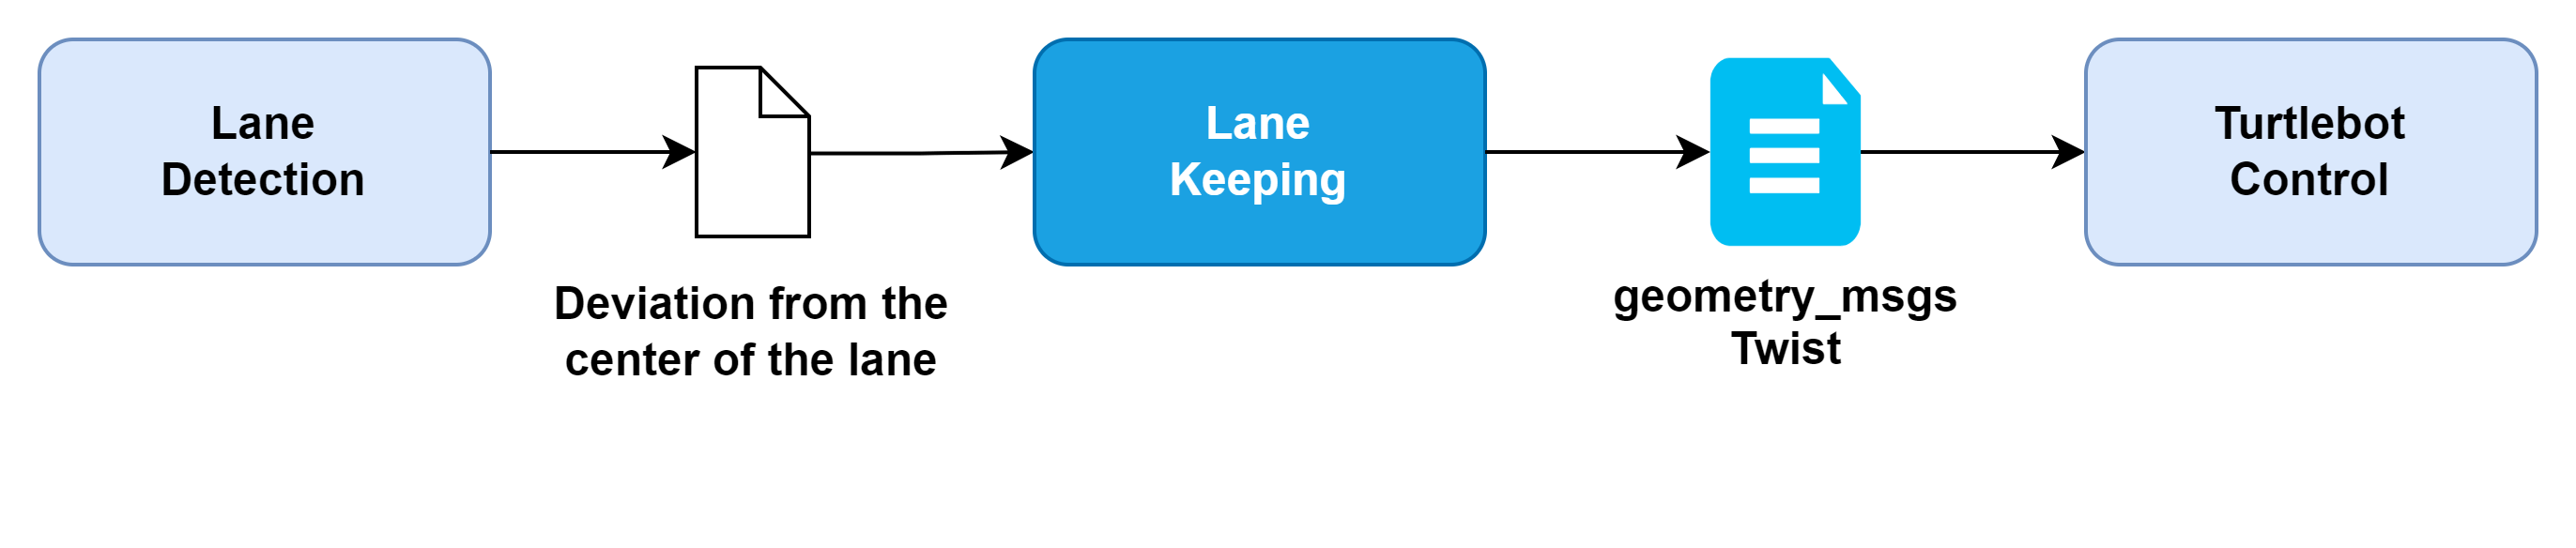
\includegraphics[width=\linewidth]{img/3_Architecture/lane_keeping_structure.png}
    \captionof{figure}{Cấu trúc của module bám làn đường}
\end{figure}

Module bám làn đường như một hàm có tham số đầu vào và đầu ra như sau:
\begin{itemize}
    \item \textbf{Input}:
    \begin{itemize}
        \item Độ lệch tâm làn đường: Tín hiệu này sẽ được gửi liên tục từ module phát hiện làn đường. Module này sẽ đảm bảo những tín hiệu gửi là đúng đắn, những tín hiệu lỗi sẽ được module nhận diện làn đường bỏ qua và gửi cảnh báo. Chính vì vậy, nếu không nhìn thấy làn đường trái hoặc phải, sẽ không trả về kết quả.
        \item Thông tin về độ lệch $d$ giữa tâm của robot so với tâm của làn đường 
    \end{itemize}
    \item \textbf{Output}: Output sẽ được gửi trực tiếp đến topic \textbf{cmd\_vel} nhằm điều khiển robot di chuyển:
    \begin{itemize}
        \item v\_linear: Vận tốc đi thẳng của robot (m/s)
        \item v\_angular: vận tốc xoay của robot (rad/s)
    \end{itemize}
\end{itemize}
\newpage
\chapter{Hiện thực hệ thống}
\section{Module nhận diện làn đường}
Nhận dạng, xác định làn đường đối các thiết bị tự hành (Autonomous vehicles) cũng như các hệ thống hỗ trợ lái xe (Driver Assistance Systems) là bài toán đặc biệt quan trong, đòi hỏi ngày càng cao về sự chính xác, an toàn ngay cả trong nhiều điều kiện khác nhau như ánh sáng, thời tiết thay đổi, sự đa dạng về môi trường hoạt động. Đối với các thiết
bị tự hành trong công nghiệp trước đây, dữ liệu đầu vào thường lấy từ các cảm biến như cảm biến hồng ngoại, cảm biến từ trường... cùng với những thiết kế cố định đối với môi trường hoạt động như ánh sáng, line đường..., điều đó làm giới hạn phạm vi hoạt động cũng như tính đa dụng của các thiết bị. Những thiết bị tự hành hiện đại hiện nay như ô tô không người lái, máy bay không người lái, robot vận chuyển hàng hóa, drone giao
hàng tự động thường sử dụng các hệ thống camera để thu thập dữ liệu cho việc xác định quỹ đạo di chuyển. Dữ liệu của camera sẽ được xử lý bằng các thuật toán xử lý ảnh hoặc các mô hình học sâu
\subsection{Các công trình liên quan}
\subsubsection{Thuật toán xử lý ảnh thông thường}
Dữ liệu từ cảm biến camera có thể được xử lý bằng các thuật toán xử lý ảnh thông thường như loc màu, phát hiện cạnh, xoay ảnh, loc nhiễu... để bóc tách được các line đường từ đó xác định được làn đường và tâm đường.
\newpage
\begin{figure}[!hbt]
\begin{center}
    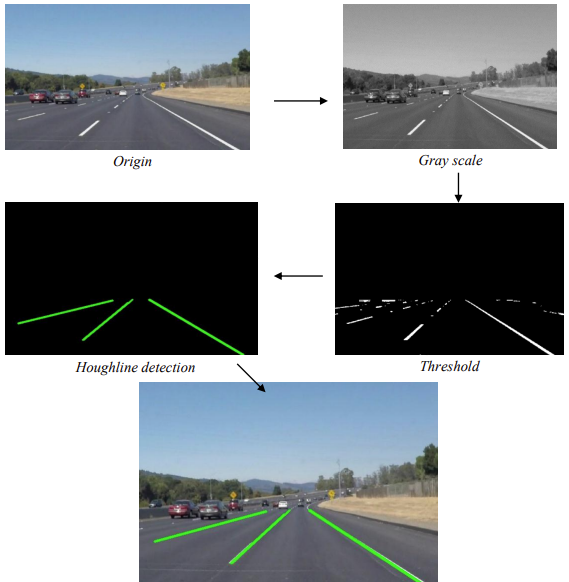
\includegraphics[width=14cm]{img/4_Implement/opencv_stages.png}
    \caption{Các giai đoạn xử lý ảnh lọc xác định làn đường sử dụng camera}
\end{center}
\end{figure}
Tuy nhiên, những thuật toán đó thường thiếu ổn định với nhiễu do độ sáng thay đổi, làn đường xuất hiện bóng cây, làn đường bị mưa ướt và thậm chí không thể xác định được làn đường khi line đường bị mất
\subsubsection{Kiến trúc học sâu}
\subsubsection{Đánh giá các model nhận diện làn đường}
Để chọn được model nhận diện làn đường phù hợp, nhóm sẽ đánh giá hiệu suất của các model khác nhau. Mục tiêu là đánh giá độ chính xác, tốc độ và độ ổn định của chúng.\\
\noindent Tập dữ liệu BDD100K\textsuperscript{\cite{bdd100k}} được sử dụng để train và đánh giá các model. Tập dữ liệu sẽ được chia thành ba phần: tập train với 70.000 ảnh, tập xác thực với 10.000 ảnh và tập đánh giá với 20.000 ảnh. Các hình ảnh sẽ được thay đổi kích thước từ 1280 × 720 xuống còn 640 × 360. Tất cả các thí nghiệm đều sử dụng framework PyTorch trên GPU NVIDIA GeForce RTX 4080.\\
\begin{table}[!hbt]
\begin{center}
\begin{tabular}{@{}cccc@{}}
\toprule
\textbf{Model} & \textbf{Kích thước} & \textbf{Params} & \textbf{Tốc độ (fps)} \\ \midrule
YOLOP\textsuperscript{\cite{yolop}}          & 640           & 7.9M            & 37                   \\
HybridNets\textsuperscript{\cite{hybridnets}}     & 640           & 12.8M           & 18                   \\
YOLOPv2\textsuperscript{\cite{yolopv2}}        & 640           & 38.9M           & 83                   \\ \midrule
TwinLiteNet\textsuperscript{\cite{twinlitenet}}    & 640           & \textbf{0.4M}   & \textbf{271}         \\ \bottomrule
\end{tabular}
\caption{\label{param-fps-table}Trọng số và tốc độ dự đoán của model}
\end{center}
\end{table}\\
Bảng \ref{param-fps-table} so sánh model TwinLiteNet \textsuperscript{\cite{twinlitenet}} với các model khác. TwinLiteNet chỉ có 0.4 triệu trọng số, ít hơn nhiều so với các model trước đây. Ngoài ra, TwinLiteNet còn đạt được 271 FPS, trong khi các model khác chỉ đạt được tốc độ dự đoán dưới 100 FPS trên cùng thiết bị.\\
\begin{table}[!hbt]
\begin{center}
\begin{tabular}{@{}ccc@{}}
\toprule
\textbf{Model} & \textbf{Độ chính xác (\%)} & \textbf{IoU (\%)} \\ \midrule
Enet\textsuperscript{\cite{enet}}                 & 34.12                      & 14.64             \\
SCNN\textsuperscript{\cite{scnn}}                 & 35.79                      & 15.84             \\
Enet-SAD\textsuperscript{\cite{enetsad}}          & 36.56                      & 16.02             \\
YOLOP\textsuperscript{\cite{yolop}}               & 70.5                       & 26.2              \\
YOLOPv2\textsuperscript{\cite{yolopv2}}           & 87.31                      & 27.25             \\
HybridNets\textsuperscript{\cite{hybridnets}}     & 85.4                       & \textbf{31.6}     \\ \midrule
TwinLiteNet\textsuperscript{\cite{twinlitenet}}   & \textbf{97.3}              & 31.08             \\ \bottomrule
\end{tabular}
\caption{\label{lane-detection-table}Kết quả nhận diện làn đường}
\end{center}
\end{table}\\
Các chỉ số được sử dụng đánh giá ở bảng \ref{lane-detection-table} là độ chính xác của pixel và IoU (Intersection over Union) của đường làn, TwinLiteNet vẫn thấp hơn HybridNets, về mặt IoU (-0.52\%), nhưng độ chính xác của TwinLiteNet đạt 97.3\%, cao hơn nhiều so với các model hiện tại. Một số kết quả segmentation của model được hiển thị trong Hình \ref{lane_visualization_results}. Cho thấy model có khả năng dự đoán mạnh mẽ cho các đường có nhiều làn, kể cả trong các tình huống ban ngày và ban đêm. Kết quả cho thấy model có khả năng dự đoán chính xác cấu hình của làn đường, không phụ thuộc vào điều kiện ánh sáng.\\
\begin{figure}[!hbt]
\begin{center}
    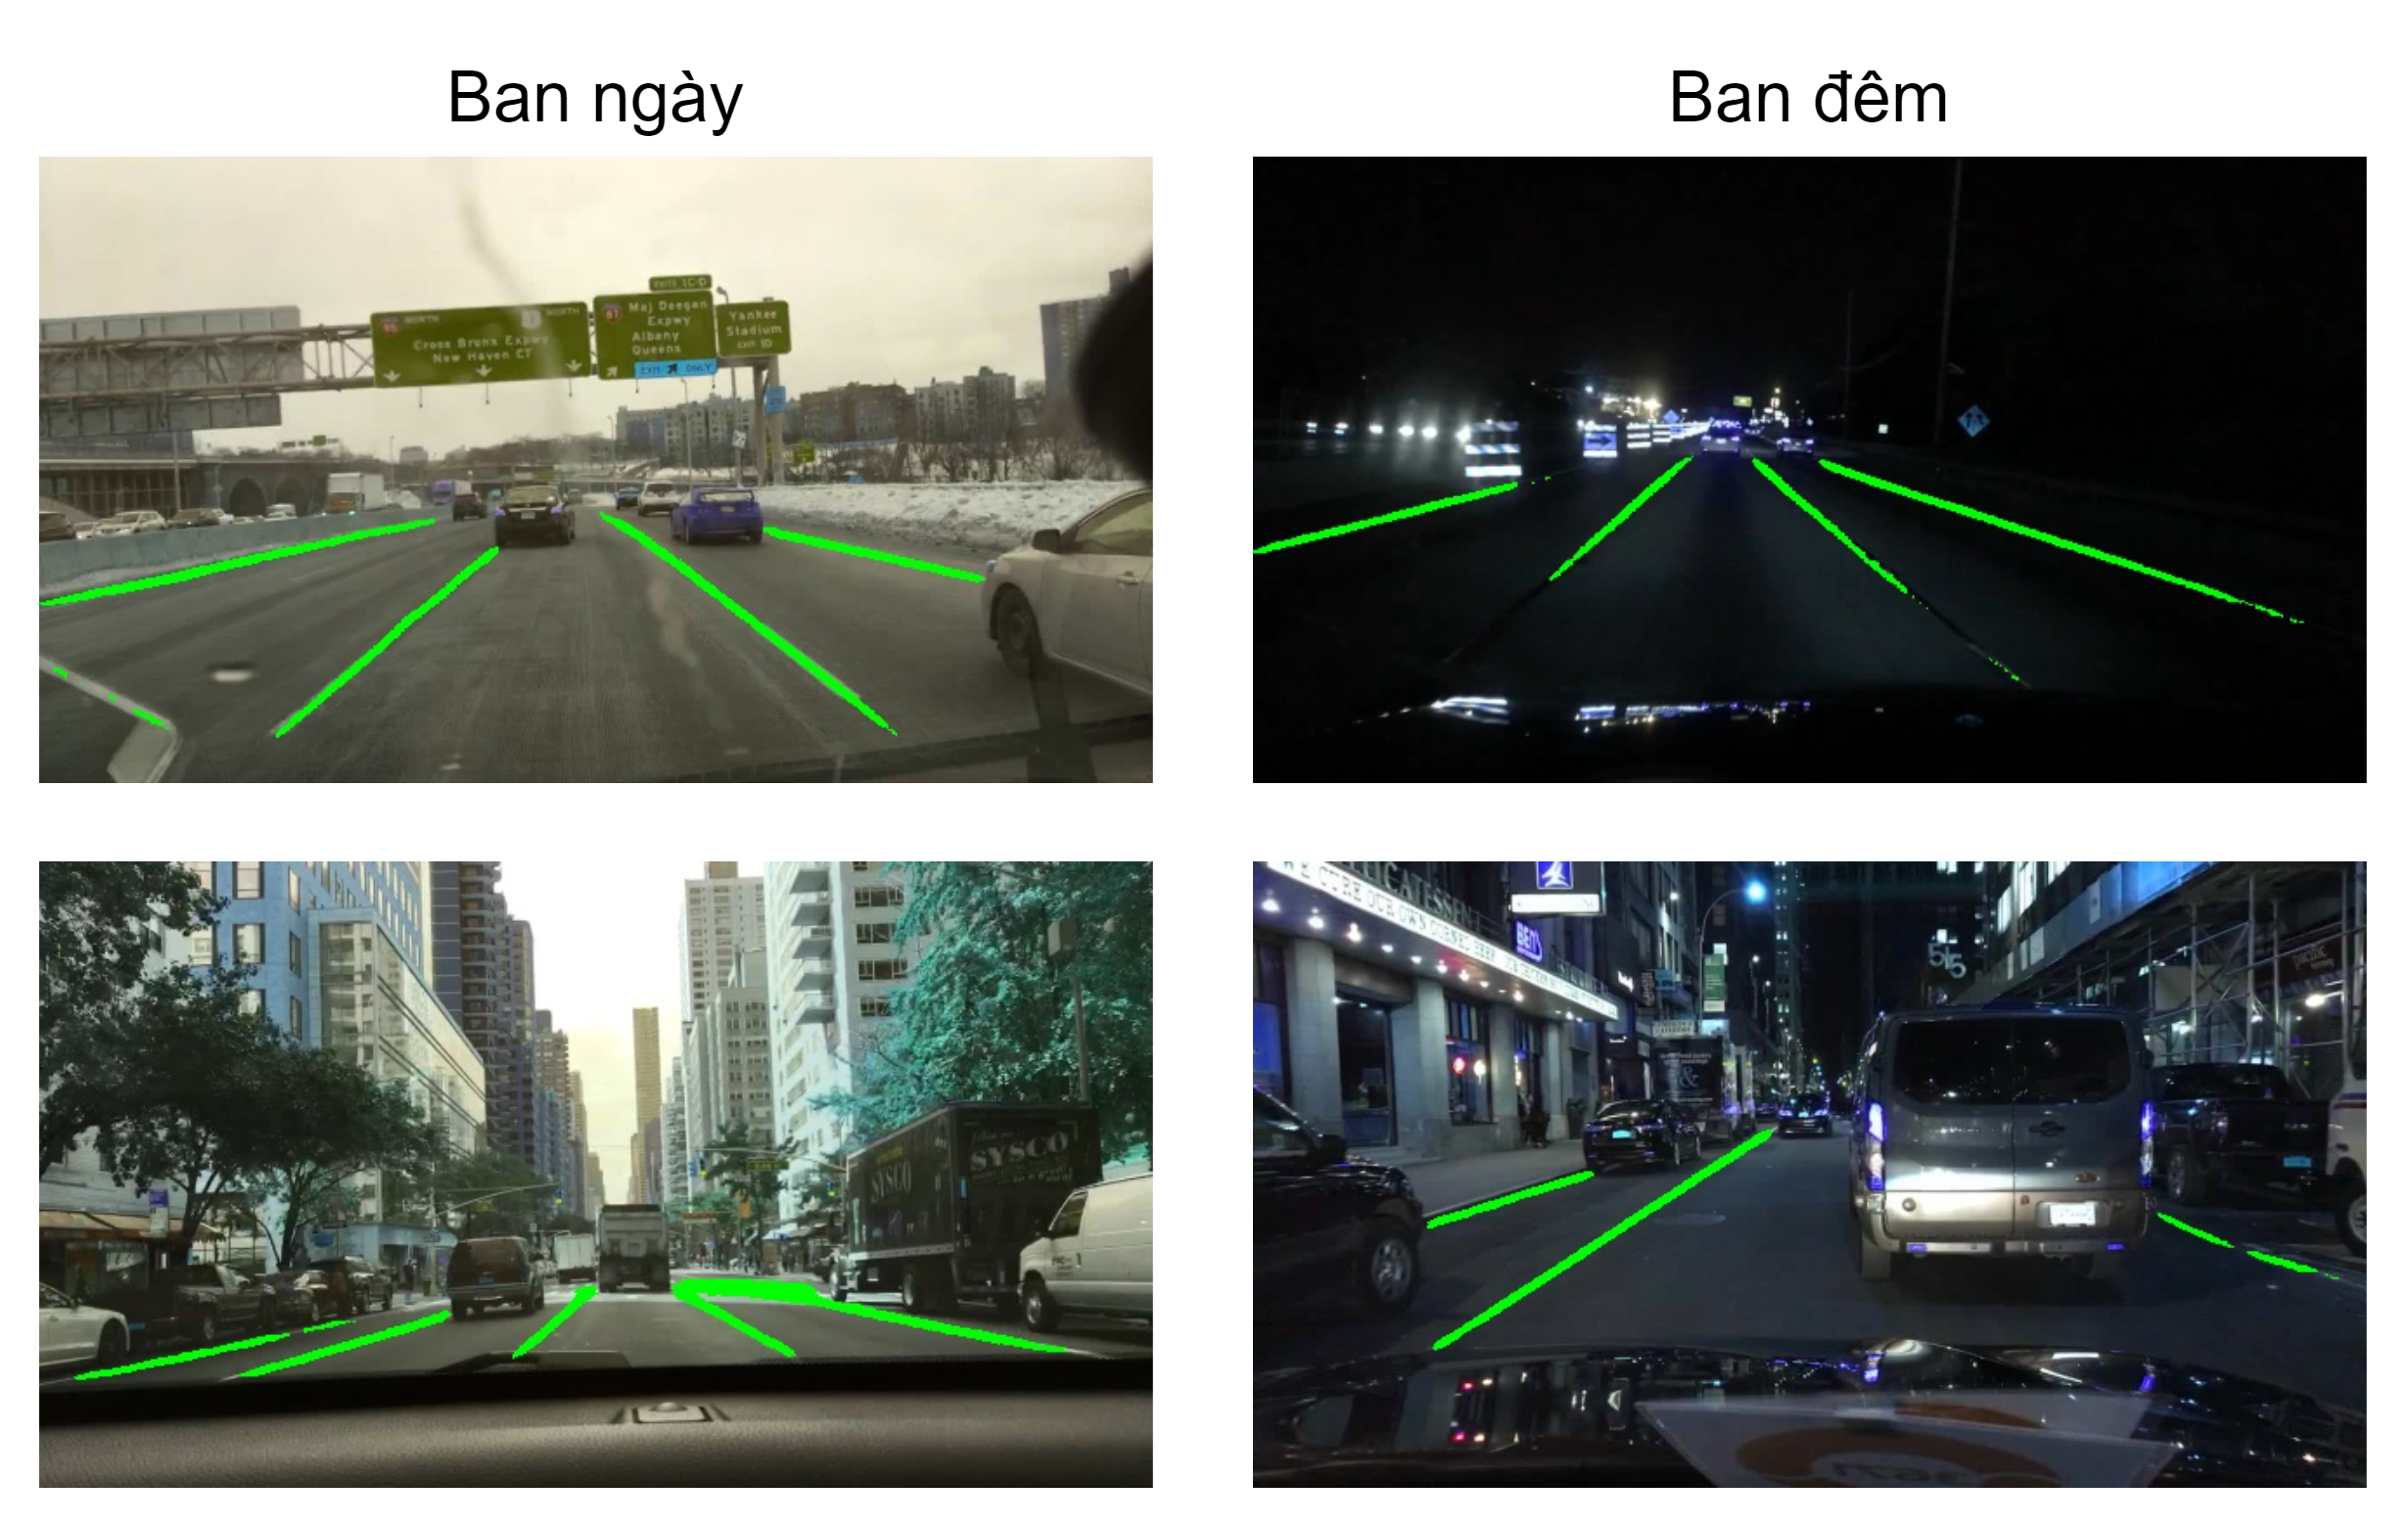
\includegraphics[width=12cm]{img/4_Implement/ai/visualization_results.png}
    \caption{\label{lane_visualization_results}Kết quả nhận diện làn đường}
\end{center}
\end{figure}\\
\subsection{Huấn luyện model}
Nhóm sử dụng model đã được train sẵn (pretrained) của tác giả, model nhận diện tốt làn đường thực tế. Tuy nhiên, vì model chỉ được huấn luyện (train) trên bộ dữ liệu thực tế nên khi nhóm thử nghiệm trên môi trường mô phỏng Gazebo\textsuperscript{\cite{gazebo}}, model đã không thể nhận diện đúng.\\
\begin{figure}[!hbt]
\begin{center}
    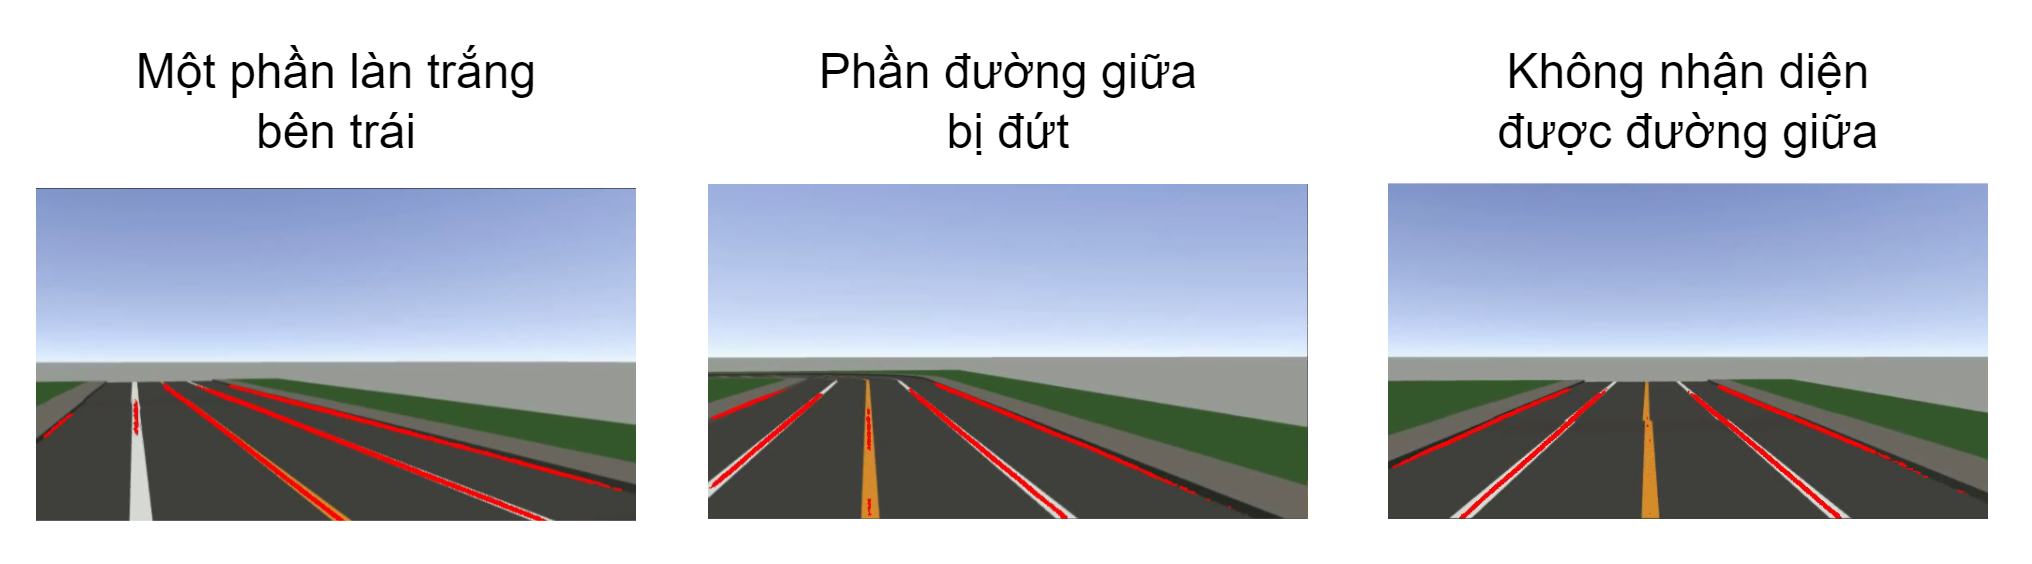
\includegraphics[width=15cm]{img/4_Implement/ai/simulation_error.png}
    \caption{Kết quả của model trước khi train thêm với data bổ sung}
\end{center}
\end{figure}\\
\textbf{Môi trường mô phỏng:}
Sau khi xác định vấn đề không thể nhận diện đúng trong môi trường mô phỏng, nhóm quyết định tiếp tục quá trình huấn luyện mô hình AI để cải thiện khả năng nhận diện của nó. Để làm điều này, nhóm đã thực hiện thu thập dữ liệu từ môi trường mô phỏng sử dụng công cụ Unity\textsuperscript{\cite{unity}}. Tổng cộng, nhóm đã thu thập 4.000 hình ảnh từ môi trường này, bao gồm các vị trí khác nhau của làn đường, vật cản, và góc độ quan sát của camera. Việc đa dạng hóa dữ liệu này giúp mô hình học được từ nhiều tình huống khác nhau, từ đó cải thiện khả năng tổng quát hóa và nhận diện trong môi trường mô phỏng. Dữ liệu thu thập từ môi trường mô phỏng sẽ được kết hợp với dữ liệu thực tế từ BDD100K\textsuperscript{\cite{bdd100k}} để tăng cường độ đa dạng và khả năng áp dụng cho cả hai môi trường thực và mô phỏng.\\\\
\textbf{Môi trường thực tế:} Với 
\noindent 
\newpage
\begin{figure}[!hbt]
\begin{center}
    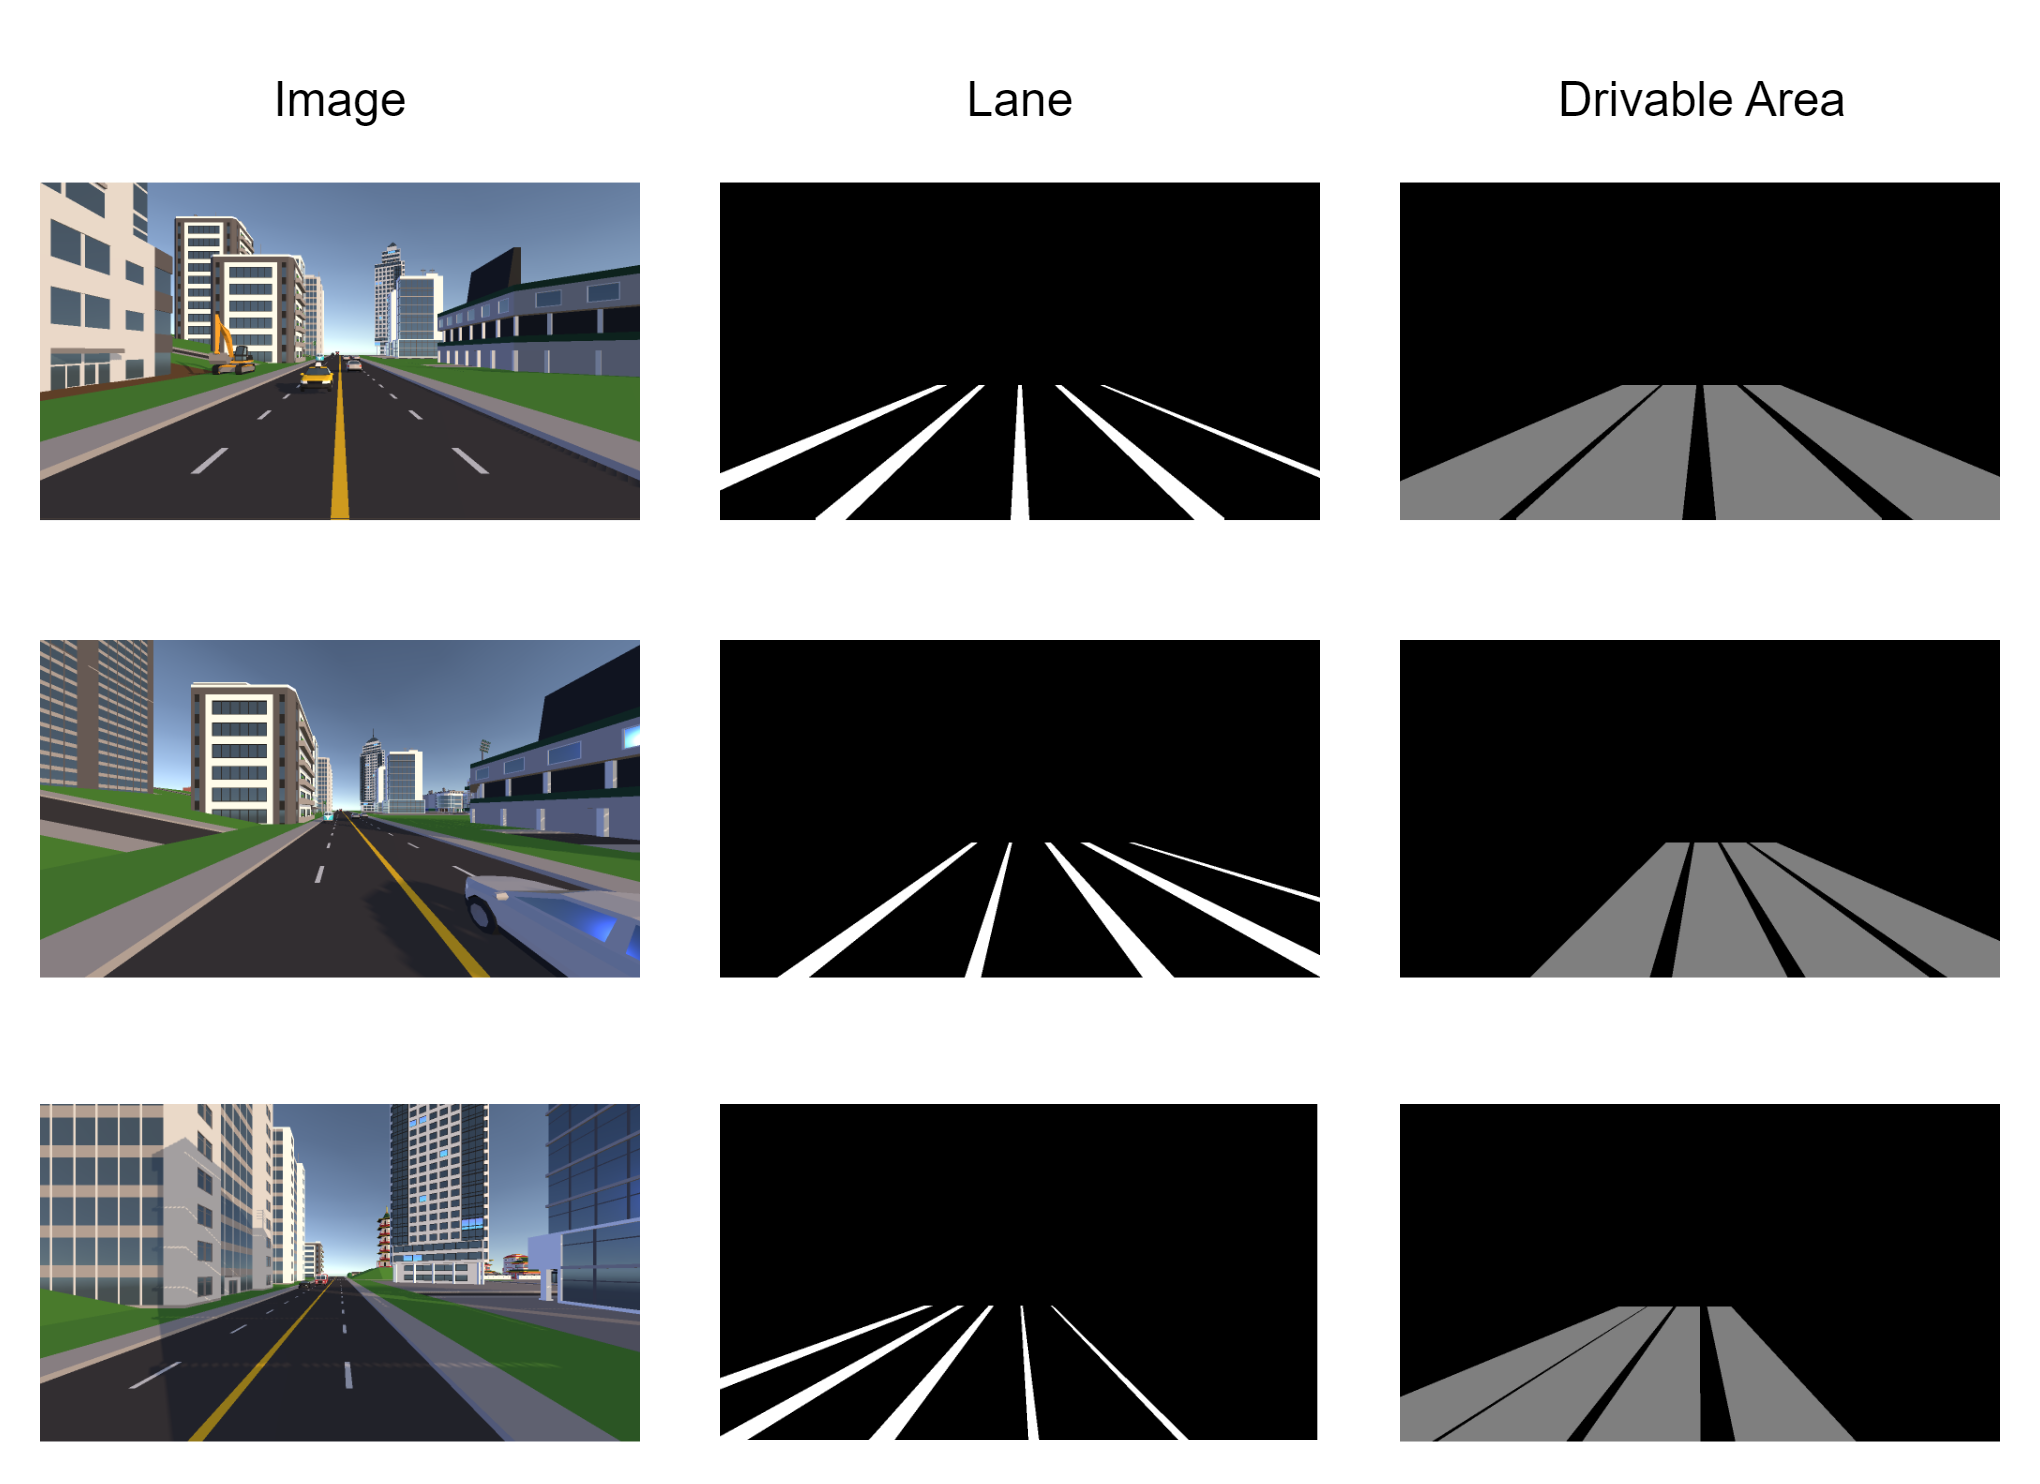
\includegraphics[width=14.5cm]{img/4_Implement/ai/simulation_data.png}
    \caption{Minh hoạ tập dữ liệu mô phỏng}
\end{center}
\end{figure}
\noindent Model sẽ được train thêm 10 epoch với batch size là 32. Qua mỗi epoch, nhóm sẽ kiểm định lại độ chính xác của model trên tập dữ liệu BDD100K. Từ đó nhóm chọn được \textbf{model\_4} (model được train thêm 4 epoch) làm model chính trong đồ án mô phỏng này
\begin{table}[!hbt]
\begin{tabular}{@{}lccccccccccc@{}}
\toprule
\textbf{Epoch}             & \textbf{0} & \textbf{1} & \textbf{2} & \textbf{3} & \textbf{4}    & \textbf{5} & \textbf{6} & \textbf{7} & \textbf{8} & \textbf{9} & \textbf{10} \\ \midrule
\textbf{Độ chính xác (\%)} & 99.0       & 99.0       & 99.0       & 98.9       & \textbf{99.0} & 98.9       & 98.5       & 98.8       & 98.3       & 98.6       & 98.4        \\
\textbf{IoU (\%)}          & 31.0       & 25.9       & 27.5       & 27.4       & \textbf{28.3} & 27.7       & 27.8       & 27.5       & 27.9       & 27.2       & 27.7        \\
\textbf{mIoU (\%)}         & 65.0       & 62.4       & 63.2       & 63.2       & \textbf{63.7} & 63.3       & 63.5       & 62.8       & 63.0       & 62.7       & 63.2        \\ \bottomrule
\end{tabular}
\caption{Thống kê đánh giá model được train thêm theo epoch}
\end{table}
\begin{figure}[!hbt]
\begin{center}
    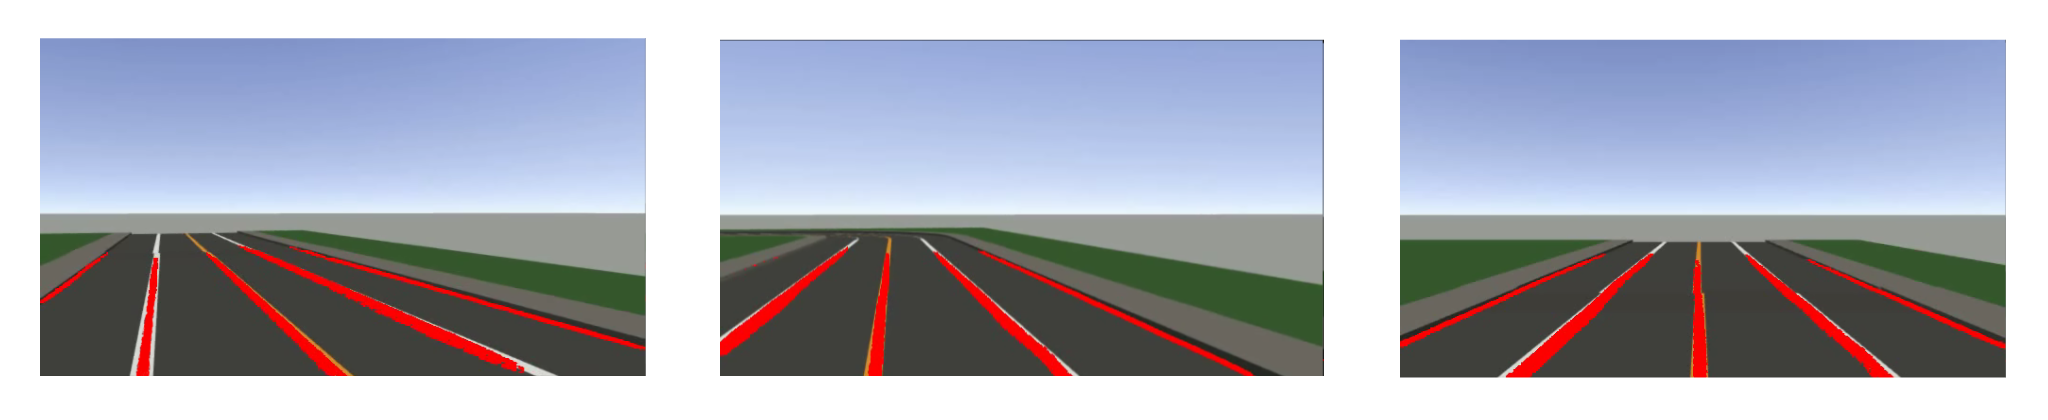
\includegraphics[width=15cm]{img/4_Implement/ai/simulation_result.png}
    \caption{Kết quả của model sau khi train thêm với data bổ sung}
\end{center}
Output hiện tại của model chỉ là ảnh RGB với hai màu trắng đen. Nhóm sẽ chuyển ảnh về dưới dạng binary để phục vụ cho quá trình phân đoạn làn đường tiếp theo. Ảnh binary là một loại hình ảnh được biểu diễn bằng các giá trị pixel chỉ có thể nhận một trong hai giá trị: 0 hoặc 1 (hoặc đen và trắng). Trong ảnh binary, mỗi pixel thường đại diện cho một phần của hình ảnh, và giá trị 0 tượng trưng cho màu đen, còn giá trị 1 tượng trưng cho màu trắng.
\end{figure}
\newpage
\subsection{Lane Fitting (Nội suy làn đường)}
Mục đích chính của module Lane Fitting là để tách các làn đường riêng biệt từ ảnh binary của model AI. Giúp ta có thể dễ dàng xác định được hình dáng, vị trí của từng làn đường.
\begin{itemize}
    \item \textbf{Input:} Kết quả nhận diện làn đường của model (dạng ảnh binary, kích thước là 640 x 360 x 1).
    \item \textbf{Output:} Trả về phương trình của tất cả làn đường 
\end{itemize}
\subsubsection{Phương pháp 1 (Hough Transform)}
\begin{figure}[h]
\begin{center}
 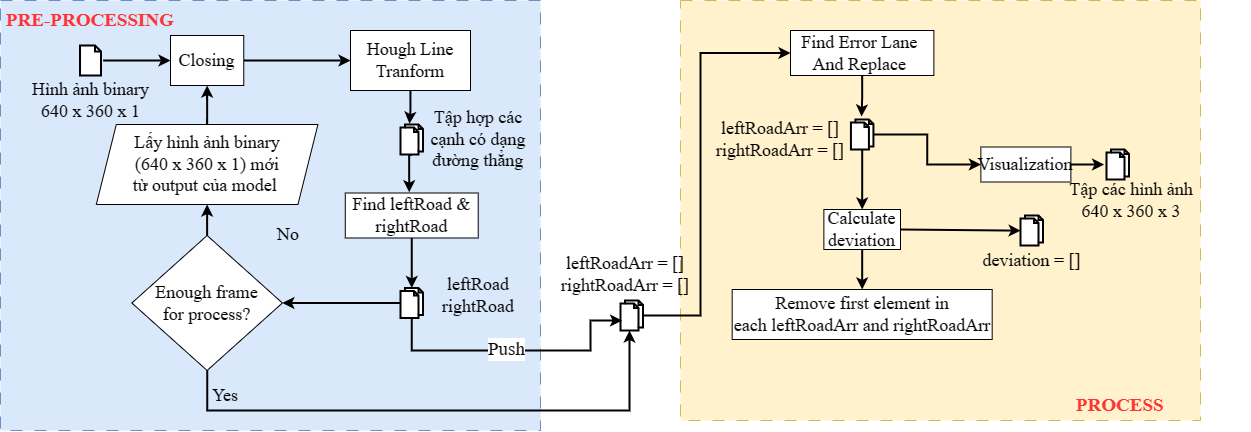
\includegraphics[width=18cm]{img/4_Implement/backend/Backend_imp.png}
 \caption{Tổng quan thuật toán của khối Backend}
 \label{back_end_cai_tien}
\end{center}
\end{figure}
\tab Dưới đây là phần giải thích chi tiết thuật toán của khối Backend sau khi được cải tiến. Khối Backend lúc này sẽ gồm 2 phần: Tiền xử lý (Pre-processing) và Xử lý (Process).\\
\tab \textbf{Pre-processing:} Khối này làm nhiệm vụ thực hiện việc tìm làn đường bên trái và làn đường bên phải của robot (không quan tâm làn đường là làn lỗi/nhiễu hay là làn đúng) cho từng ảnh (frame) trên tổng số \textbf{N} (với \textbf{N} là một ngưỡng số lượng các ảnh cần lấy để quá trình \textbf{Xử lý} đưa ra kết quả đúng nhất). Sau khi thực hiện Pre-processing trên \textbf{N} ảnh, tiến hành \textbf{Xử lý}.\\
\tab \textbf{Input:}
\begin{figure}[h]
    \centering
    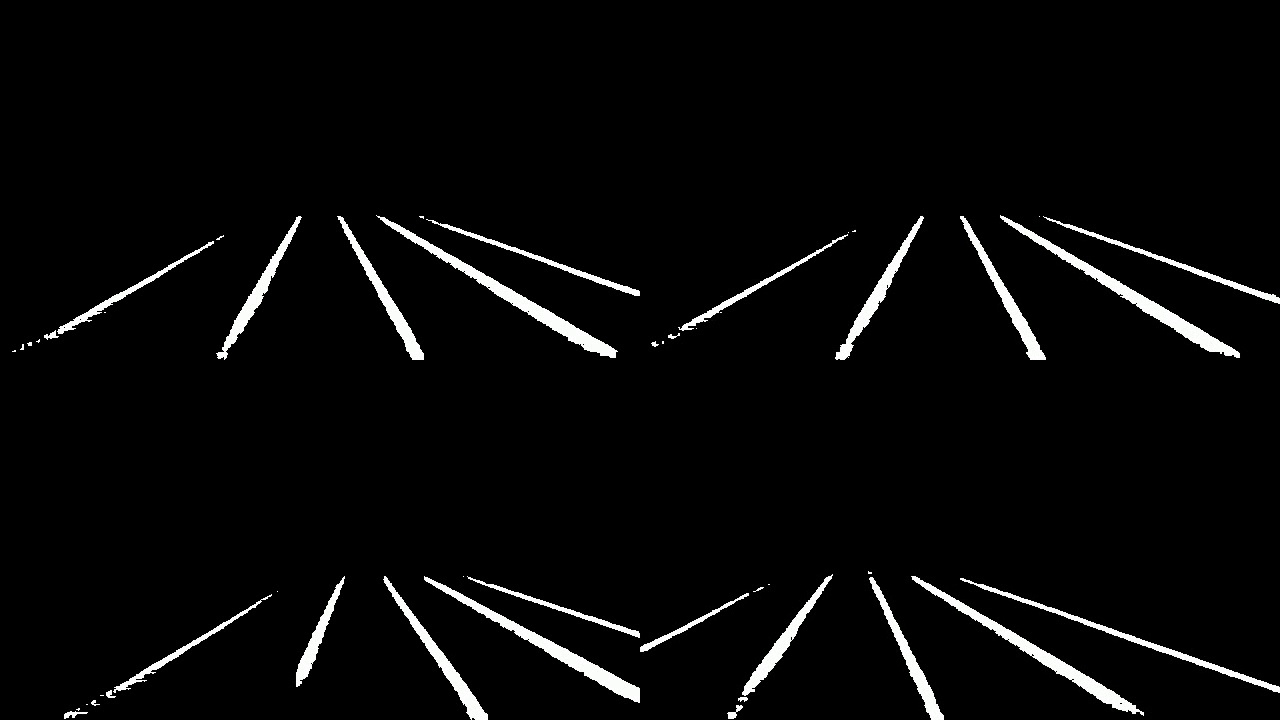
\includegraphics[width = 12cm]{img/4_Implement/backend/input.png}
    \caption{Hình ảnh minh họa cho input}
\end{figure}
\begin{enumerate}
    \item Lấy 1 ảnh mới. Tiến hành các bước 2 - 4 trên hình này.
    \item \textit{Ứng dụng Closing:} nhằm làm mịn các đường viền, đóng các lỗ nhỏ và giảm nhiễu trong ảnh.
    \begin{figure}[h]
        \centering
        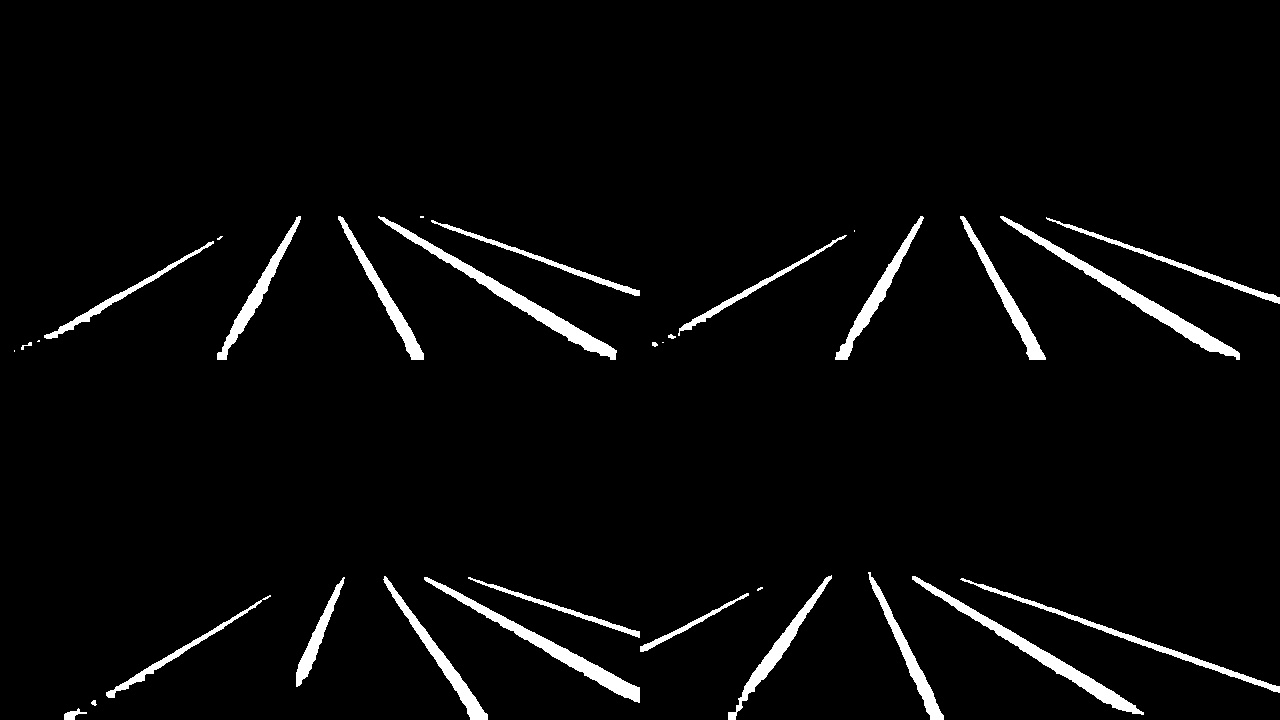
\includegraphics[width=12cm]{img/4_Implement/backend/closing.jpg}
        \caption{Hình ảnh minh họa cho làn đường sau khi ứng dụng Closing}
    \end{figure}
    \item \textit{Sử dụng thuật toán Hough Line Transform\textsuperscript{\cite{houghtransform}}:} Tìm kiếm những cạnh có dạng đường thẳng. Các đường được chia làm ba loại dựa theo góc  $\theta$ hợp giữa đường thẳng và trục hoành (Ox):
    \begin{itemize}
        \item Đường thẳng thuộc về phía bên trái có góc $\theta$ < 0.
        \item Đường thẳng thuộc về phía bên phải có góc $\theta$ > 0.
        \item Đường thẳng không thuộc về làn bên phải lẫn làn bên trái - đường nằm ngang, góc $\theta = 0$.
    \end{itemize}
    Từ tập các cạnh có dạng đường thẳng sinh ra từ thuật toán Hough Line Transform, ta thu được 2 tập đường thẳng con: 1 tập đường thẳng thuộc về làn đường phía bên trái và 1 tập đường thẳng thuộc về làn đường phía bên phải. Ta gọi tập đường thẳng thuộc phía bên trái là $L_{left} = \{ L_0, L_1,.., L_{k-1}\}$, (với $k$ là số lượng đường thẳng thỏa mãn điều kiện thuộc về làn đường phía bên trái) và tập đường thẳng thuộc phía bên phải là $L_{right} = \{L_0, L_1,.., L_{m-1}\}$ (với $m$ là số lượng đường thẳng thỏa mãn điều kiện thuộc về làn đường phía bên phải).
    \begin{figure}[h]
        \centering
        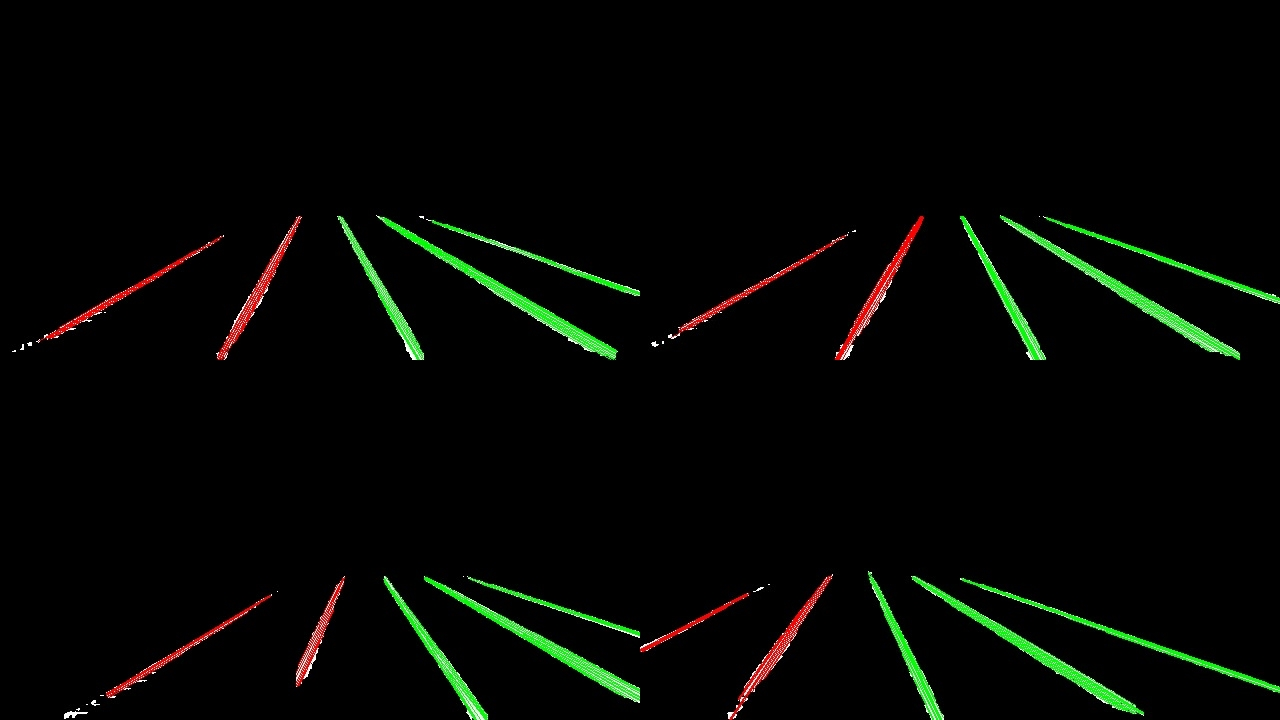
\includegraphics[width=12cm]{img/4_Implement/backend/hough_line.jpg}
        \caption{Hình ảnh minh họa làn đường sau khi ứng dụng Hough Line Transform}
    \end{figure}
    \item \textit{Find leftRoad và rightRoad}: Xác định 01 làn đường trái và 01 làn đường phải của robot. Cách xác định như sau:
    \begin{itemize}
        \item Tìm trong tập $L_{left}$ 01 đường thẳng sao cho trị tuyệt đối của góc $\theta$ hợp bởi đường thẳng này và trục hoành có giá trị lớn nhất. Ta nhận đường thẳng này là làn đường phía bên trái của robot. Gọi đường thẳng này là leftRoad. Trong trường hợp không tìm thấy đường thẳng (do mất toàn bộ làn đường bên trái), leftRoad lúc này không tồn tại.
        \item Tìm trong tập $L_{right}$ 01 đường thẳng sao cho  góc $\theta$ hợp bởi đường thẳng này và trục hoành có giá trị lớn nhất. Ta nhận đường thẳng này là làn đường phía bên phải của robot. Ta gọi đường thẳng này là rightRoad. Trong trường hợp không tìm thấy đường thẳng (do mất toàn bộ làn đường bên phải), rightRoad lúc này không tồn tại.
    \end{itemize}
    Lúc này, ta được leftRoad và rightRoad lần lượt là đường thẳng thuộc làn đường bên trái và đường thẳng thuộc làn đường bên phải của robot, kết quả này có thể bao gồm cả đường thẳng thuộc trường hợp nhiễu hoặc không tồn tại. Ta thêm leftRoad vào tập các làn đường bên trái và rightRoad vào tập các làn đường bên phải nhằm phục vụ cho các bước xử lý tiếp theo. Nếu chưa đủ \textit{N} frame, quay lại bước 1. Nếu đã đủ, qua bước \textbf{Xử lý}.    
\end{enumerate}
\tab \textbf{Xử lý:} Nhiệm vụ của bước này là lọc ra những đường thẳng lỗi và thay thế chúng (nếu có). Chi tiết bước này trình bày như sau:
\begin{enumerate}
    \item \textit{Find error line and replace:} Ta tiến hành tìm kiếm và thay thế những đường thẳng lỗi cho làn đường bên trái và làn đường bên phải như sau:

    
    \begin{itemize}
        \item Gọi $\theta_{n}^{l}$ là trị tuyệt đối của góc hợp bởi đường thẳng bất kì thuộc tập làn đường bên trái (thu được từ bước \textbf{Xử lý} trước đó) với trục hoành. 
        \item Gọi $\theta_{n}^{r}$ là góc hợp bởi đường thẳng bất kì thuộc tập làn đường bên phải trước đó (thu được từ bước \textbf{Xử lý} trước đó) với trục hoành .
        % \item $\theta_{l} = [|\theta_{0}^{l} - \theta_{n}^{l}|, |\theta_{1}^{l} - \theta_{n}^{l}|,...|\theta_{k-1}^{l} - \theta_{n}^{l}|]$. Với k là số lượng đường thẳng có trong tập làn đường bên trái đang xử lý, k $\leq$ \textit{num}.
        % \item $\theta_{r} = [|\theta_{0}^{r} - \theta_{n}^{r}|, |\theta_{1}^{r} - \theta_{n}^{r}|,...|\theta_{m-1}^{r} - \theta_{n}^{r}|]$. Với m là số lượng đường thẳng có trong mảng làn đường bên phải đang xử lý, m $\leq$ \textit{num}.
        \item Gọi $\theta_{i}^{l}$ là góc hợp bởi đường thẳng thứ $i$ ($i = \{0,1,...,N-1\}$) thuộc tập làn đường bên trái với trục hoành.
        \item Gọi $\theta_{i}^{r}$ là góc hợp bởi đường thẳng thứ $i$ ($i = \{0,1,...,N-1\}$) thuộc tập làn đường bên phải với trục hoành.
        \item Gọi $\gamma$ là ngưỡng chấp nhận được. Cụ thể hơn: $|\theta_{i}^{l} - \theta_{n}^{l}| < \gamma$ và $|\theta_{i}^{r} - \theta_{n}^{r}| < \gamma$, với $i = \{0,1,...,N-1\}$. Những đường thẳng có trị tuyệt đối của hiệu lớn hơn sẽ được xem là những đường thẳng lỗi, và sẽ được thay thế bằng đường thẳng đứng trước nó (trong tập). Tuy nhiên, với những trường hợp không thể tính góc $\theta$ do đường thẳng không tồn tại, chương trình sẽ trả về "Không nhận diện được".
    \end{itemize}
    Kết quả cuối cùng của bước này, ta thu được tập các làn đường bên trái $L_{l} = \{ L_0, L_1,.., L_{k-1}\}$ và tập các làn đường bên phải $L_{r} = \{L_0, L_1,.., L_{k-1}\}$, $k \leq N$ chỉ bao gồm những làn đường đúng.
    \item \textit{Calculate deviation:} Từ tập các đường thẳng bên trái và mảng các làn đường bên phải, ta lấy ra leftRoad thứ $i$ và rightRoad thứ $i$, $i = \{0,1,...,N-1\}$, ta có thể tính được độ lệch của robot so với tâm làn đường thứ i như sau:
    \begin{itemize}
        \item Tìm giao điểm của leftRoad với trục hoành. Gọi điểm này là $it_{l}$.
        \item Tìm giao điểm của rightRoad với trục hoành. Gọi điểm này là $it_{r}$.
        \item Tìm phương trình đường thẳng của làn đường trung tâm: Là đường thẳng nối 2 điểm: giao điểm của leftRoad và rightRoad với trung điểm của $it_{l}$ và $it_{r}$
        \item Tính độ dài hình chiếu của đường thẳng này xuống trục hoành. Độ dài của hình chiếu chính là độ lệch $d$ chúng ta cần tìm.
    \end{itemize}
    Kết quả của bước này là mảng các giá trị \textit{d} tương ứng với các frame.
    \item \textit{Visualization:} Từ tập các đường thẳng bên trái và tập các làn đường bên phải, ta lấy ra leftRoad thứ $i$ và rightRoad thứ $i$, $(0 \leq i \leq k-1)$, $k \leq N$, ta có thể visualize kết quả nhận diện làn đường trái và làn đường phải của khối Backend cải tiến lên ảnh thứ i tương ứng. Kết quả như hình \ref{final_result_of_BE}.
    \begin{figure}[h]
        \centering
        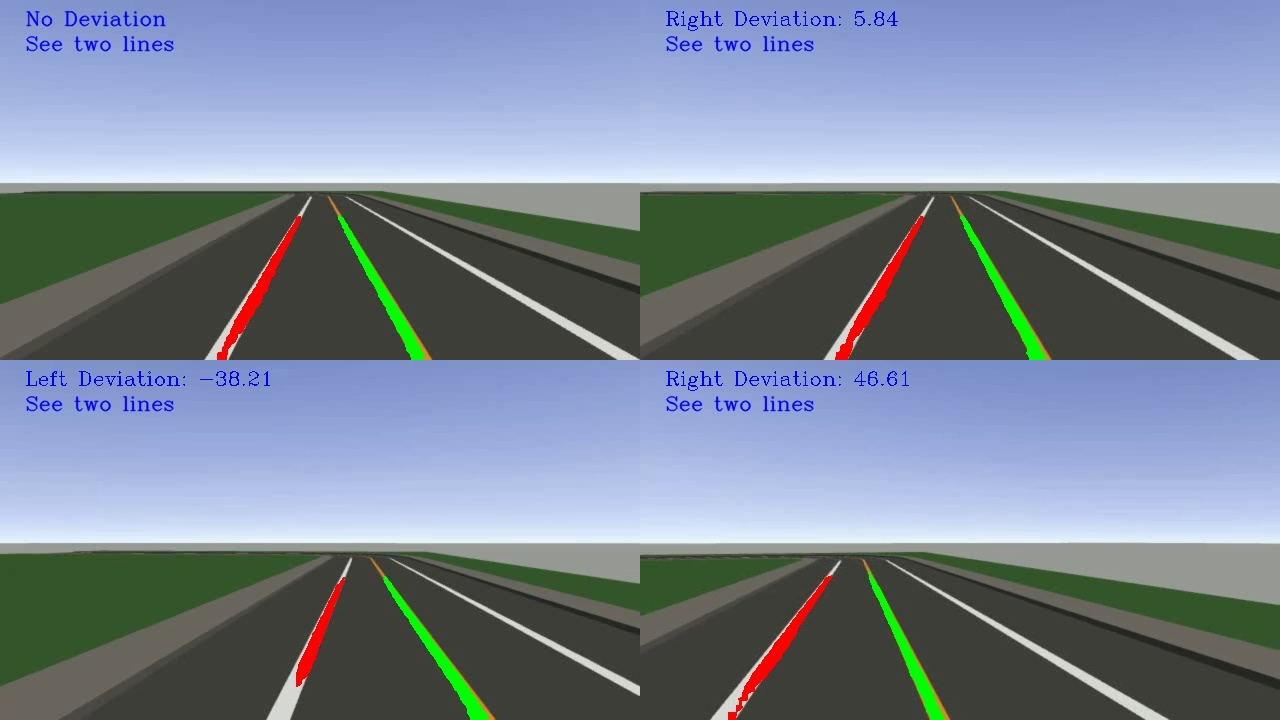
\includegraphics[width=12cm]{img/4_Implement/backend/ressult.jpg}
        \caption{Hình ảnh kết quả cuối cùng của khối Backend}
        \label{final_result_of_BE}
    \end{figure}
    \item Xóa phần tử đầu tiên của mảng làn đường bên trái và mảng làn đường bên phải.
\end{enumerate}
\textbf{Ưu điểm và nhược điểm}
\subsubsection{Phương pháp 2 (K–means Clustering)}
\textbf{Ưu điểm và nhược điểm}
\subsubsection{Phương pháp 3 (Sliding Window)}
Bởi vì số cluster không thể xác định do các cụm làn đường luôn luôn thay đổi. Do đó, nhóm đã chuyển sang sử dụng phương pháp sliding window. Với sliding window, ta có thể linh hoạt xác định các vùng có khả năng chứa làn đường trên ảnh.\\\\
\textbf{Perspective Transform:}\
Trước khi áp dụng sliding window, ta cần thực hiện biến đổi \textbf{camera view} sang \textbf{bird’s eye view}, giúp thuận tiện cho việc phân đoạn và xác định làn đường. Khi nói về Affine Transformations, chúng ta nói đến một loại phép biến đổi hình học trong không gian hai hoặc ba chiều. Khi áp dụng phép biến đổi này, các điểm trong không gian được di chuyển, xoay và co giãn để tạo thành một hình học mới. Điều này có thể được biểu diễn bằng ma trận biến đổi affine.\\\\
Ma trận biến đổi Affine được biểu diễn dưới dạng ma trận $3x3$ cho biến đổi trong
không gian hai chiều. Ma trận này bao gồm các thông số để biểu diễn các phép biến đổi
như dịch chuyển, xoay và co giãn. Cụ thể, ma trận Affine cho phép dịch chuyển bằng
cách thêm một vector tịnh tiến vào tọa độ ban đầu của điểm. Xoay được thực hiện bằng
cách sử dụng các phép toán ma trận để xoay điểm quanh một trung tâm quay. Co giãn
được thực hiện bằng cách thực hiện phép nhân ma trận với một vector giữa các hệ số co
giãn tương ứng cho mỗi chiều.\\\\
Những vị trí này sẽ tương ứng với những vị trí xác định trong bề mặt bird’s eye view. Vậy nhóm sẽ có bốn cặp điểm ở bề mặt thực tế tương ứng với bề mặt bird’s eye view. Nhóm sử dụng hàm \textbf{cv2.getPerspectiveTransform} để suy ra được ma trận biến đổi affine từ bốn cặp điểm trên. Ma trận này đặc trưng cho vị trí của camera so với robot và bề mặt nằm ngang, do đó các thay đổi như thay đổi về chiều cao robot hoặc vị trí camera, nhóm sẽ phải thực hiện lại bước thiết lập các điểm để đảm bảo tính đúng đắn của ma trận affine.
\newpage
\begin{figure}[!hbt]
\begin{center}
    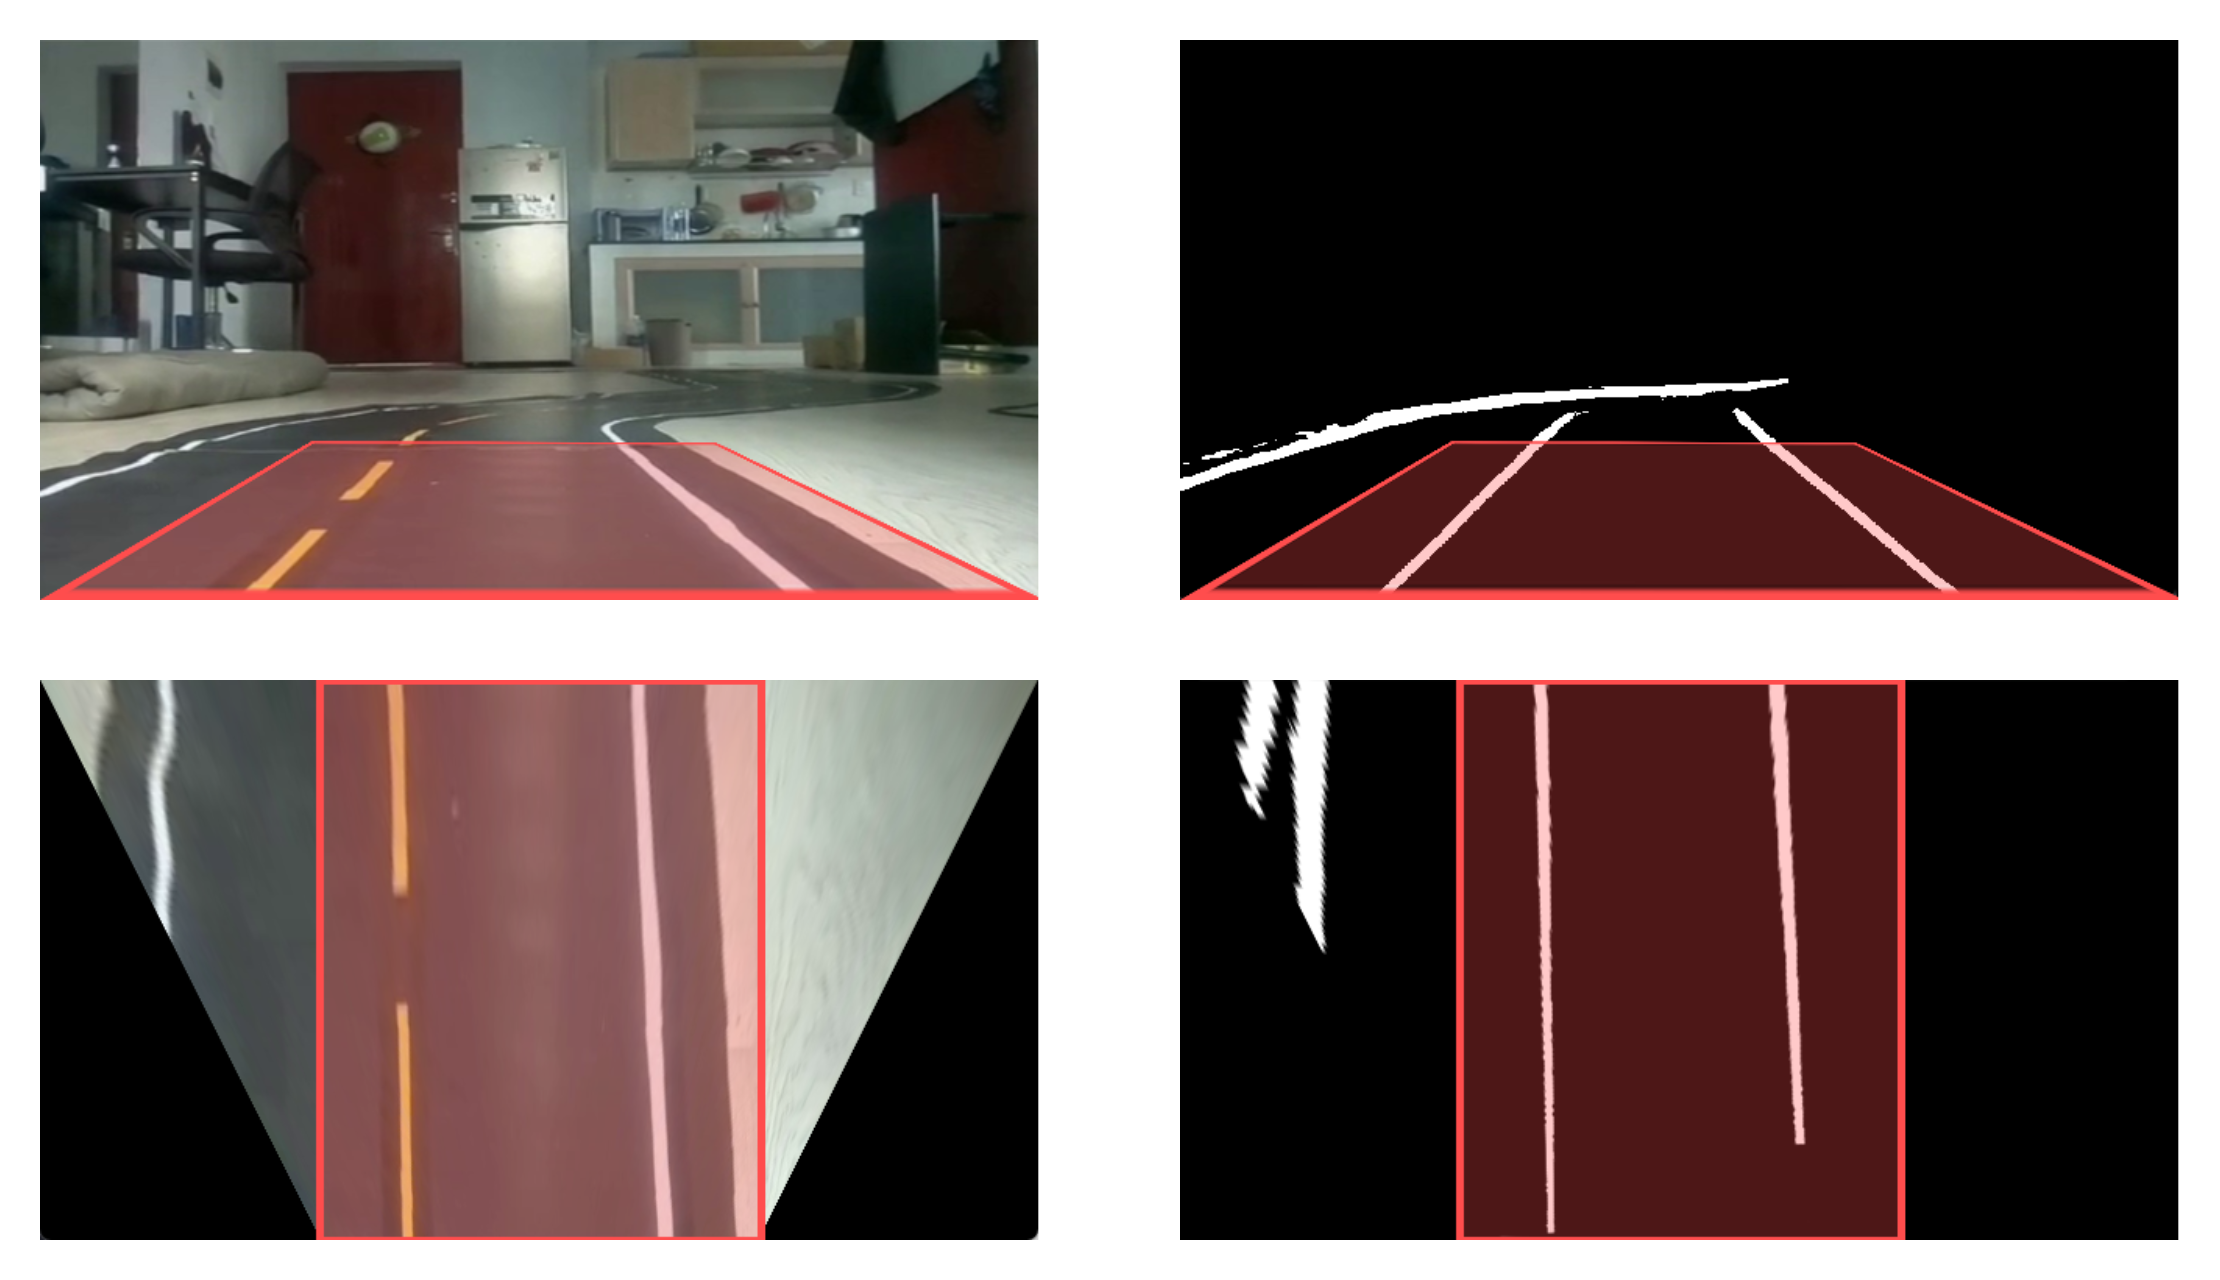
\includegraphics[width=15cm]{img/4_Implement/sliding_window/perspective_transform.png}
    \caption{Ảnh từ camera view và bird's eye view}
\end{center}
\end{figure}
\noindent Vị trí bốn điểm ở hệ toạ độ camera: $\begin{bmatrix}190 & 250\\460 & 250\\640 & 360\\0 & 360\end{bmatrix}$\\
Vị trí bốn điểm ở hệ toạ độ thực: $\begin{bmatrix}180 & 100\\460 & 100\\460 & 360\\180 & 360\end{bmatrix}$\\
Ma trận affine thu được: $M = \begin{bmatrix}-0.5 & -1.9 & 484.97\\-5.33 & -3.24 & 762.42\\-1.43 & -0.005 & 1.0\\\end{bmatrix}$\\
Khi đã có ma trận affine, Ta chuyển một điểm từ hệ toạ độ camera ($x_1$, $y_1$) sang hệ toạ độ
bird eye's view ($x_2$, $y_2$) như sau:
\begin{equation}
    \begin{bmatrix}x_2\\y_2\\1\end{bmatrix} = \begin{bmatrix}x_1\\y_1\\1\end{bmatrix}M
\end{equation}
Ta có $M_{inv}$ là ma trận đảo ngược của $M$ để biến đổi dữ liệu từ hệ toạ độ bird eye's view về hệ toạ độ camera, thuận tiện cho việc visualize kết quả \\\\
\textbf{Sliding Window:}
Dưới đáy của ảnh binary, một sliding window có chiều rộng bằng chiều rộng của ảnh sẽ di chuyển từ dưới lên trên cho đến khi tìm thấy cụm pixel đầu tiên của làn đường. Cụm pixel đầu tiên này được xác định là điểm bắt đầu của một làn đường. Từ cụm pixel này, một sliding window thứ hai được sử dụng để trích xuất tất cả các pixel thuộc về làn đường đó. Mặc dù chiều cao của cửa sổ này giống như cửa sổ trước, tuy nhiên, chiều rộng sẽ lớn hơn một chút so với chiều rộng của cụm pixel đầu tiên. Sau khi sliding window thứ hai đã được áp dụng, các cụm pixel của làn đường đó sẽ được loại bỏ khỏi ảnh. Quá trình này sẽ được lặp lại cho đến khi tất cả các làn đường đã được trích xuất hoàn toàn.\\
\begin{figure}[!hbt]
\begin{center}
    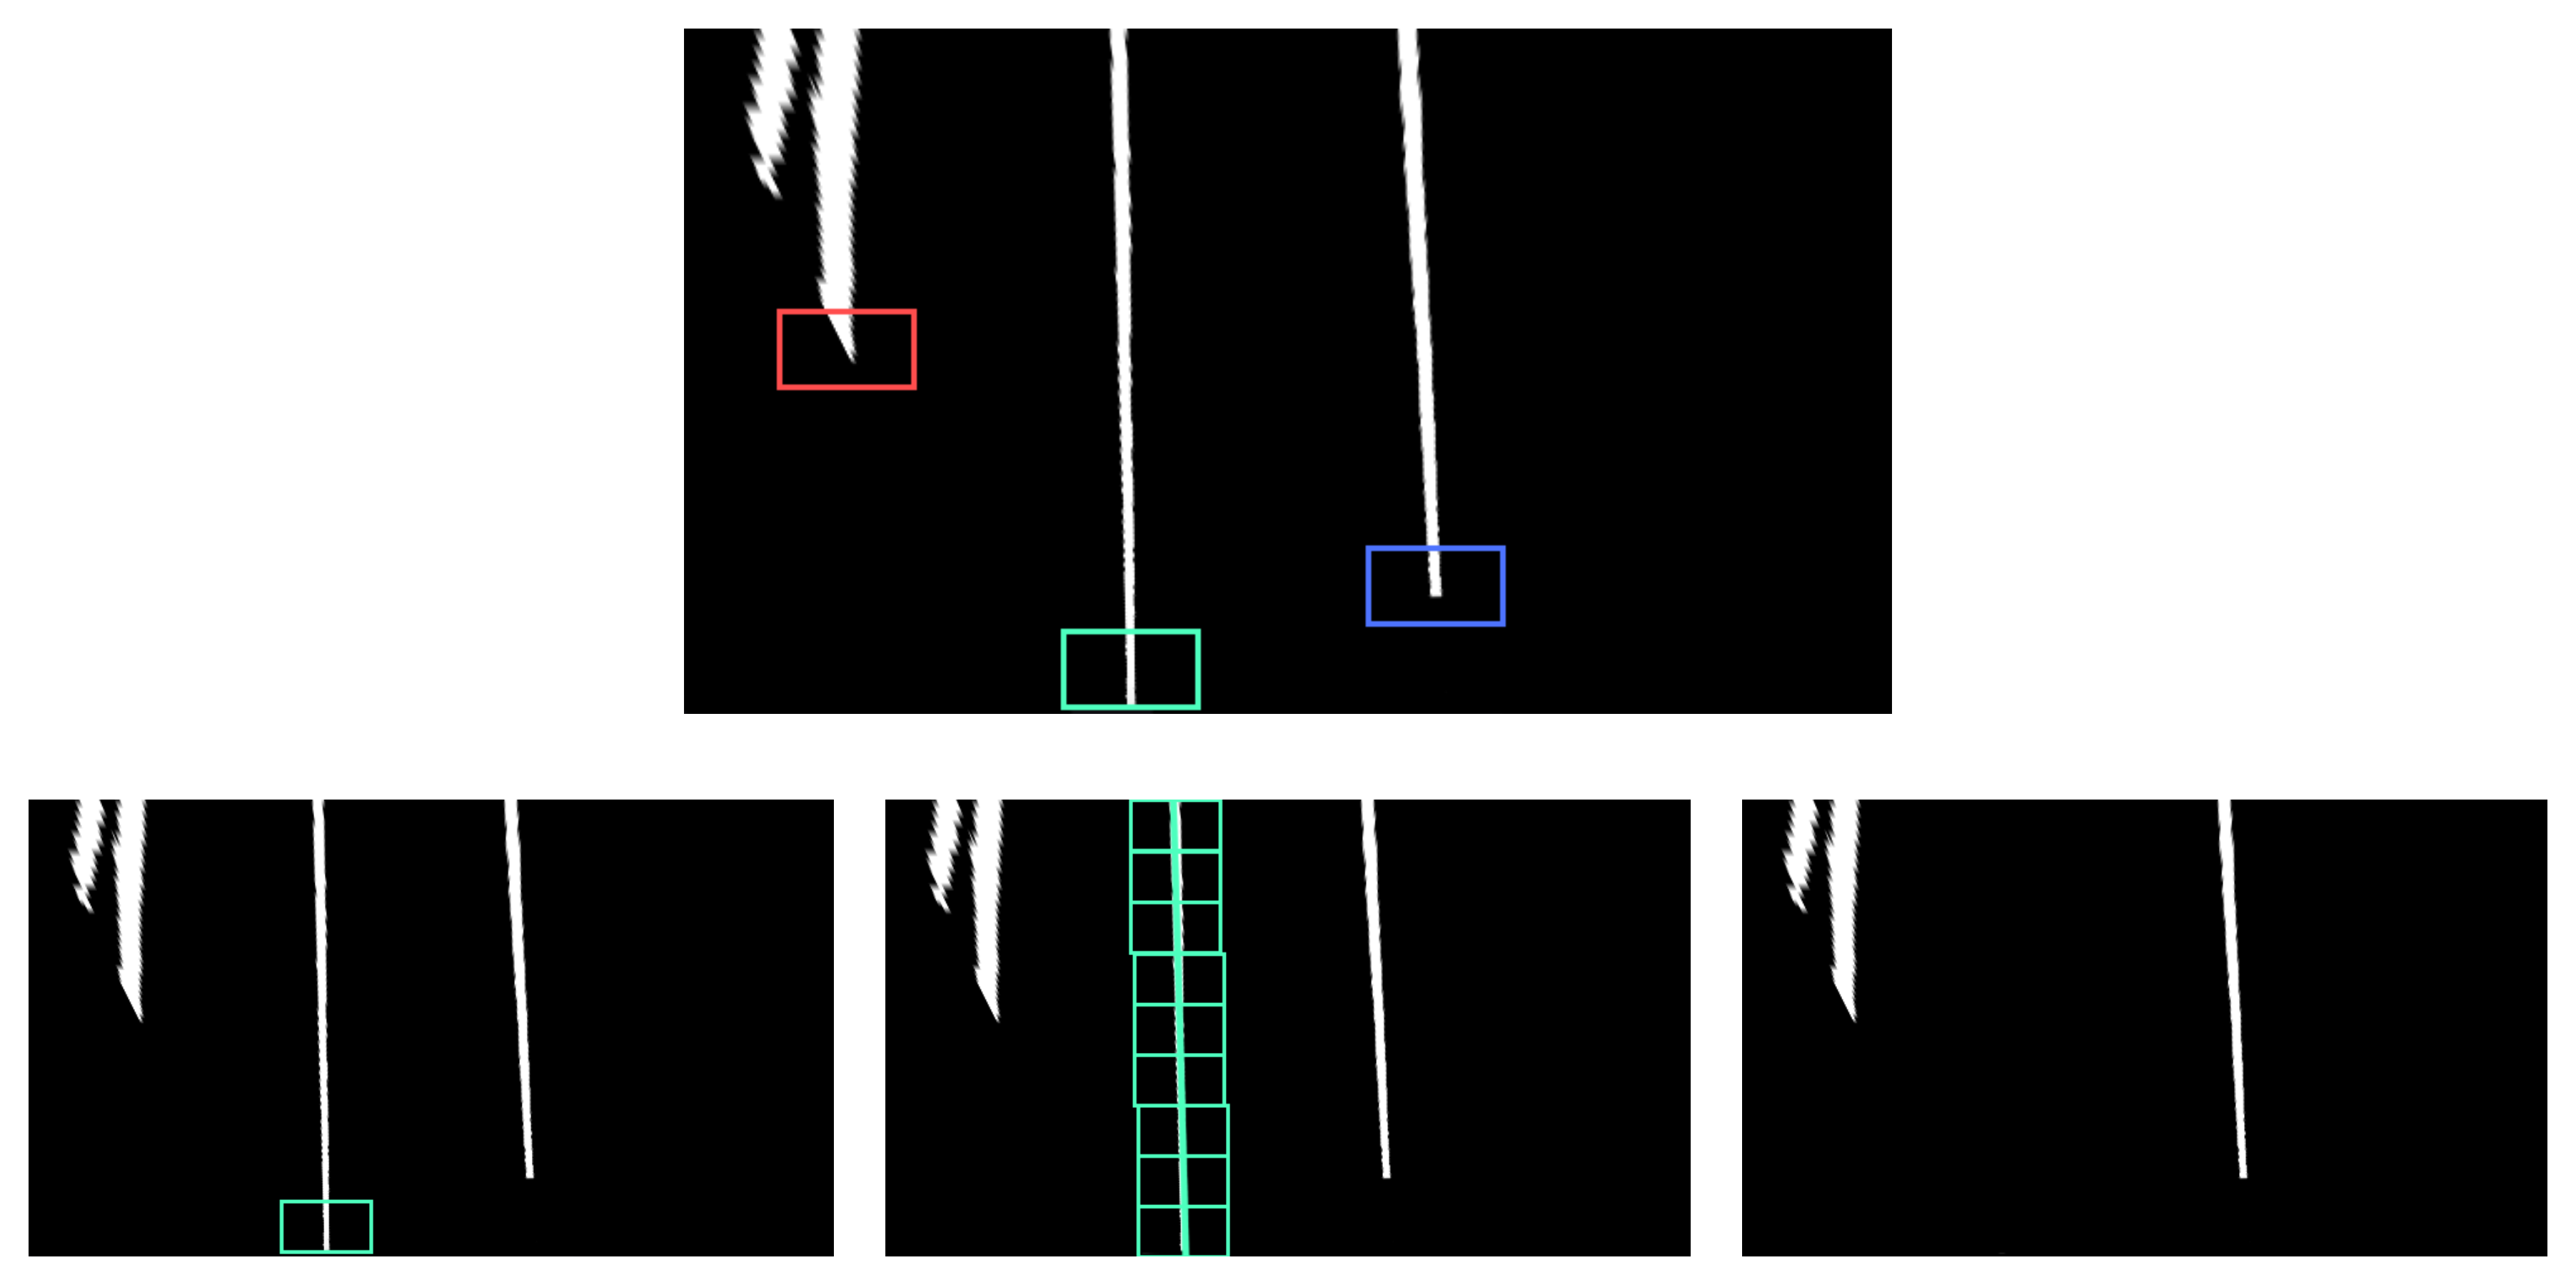
\includegraphics[width=15cm]{img/4_Implement/sliding_window/fitting.png}
    \caption{(a) Sliding window thứ nhất tìm cụm pixel đầu tiên; (b) Sliding widow thứ hai bắt đầu tại cụm pixel đầu tiên; (c) Sliding window tìm tất cả cụm pixel làn đường; (d) Xoá các cụm pixel của làn đường và lặp lại bước a}
\end{center}
\end{figure}\\
Nhóm đã cải tiến thêm thuật toán để bỏ qua việc trích xuất làn đường trong các trường hợp sau:
\begin{itemize}
    \item Làn đường trích xuất có độ dài ngắn
    \item Hai làn đường kế tiếp nhau có khoảng cách quá nhỏ so với độ rộng của robot
    \item Thiết lập ngưỡng tối đa làn đường có thể trích xuất
\end{itemize}
Các cải tiến này giúp tăng cường hiệu suất và độ chính xác của thuật toán, đồng thời giảm thiểu các trường hợp sai sót và tối ưu hóa quá trình trích xuất làn đường\\\\
\textbf{Curve Fitting:}
Sau khi một làn đường được trích xuất, ta có thể dễ dàng dùng hồi quy tuyến tính để nội suy làn đường. Phương trình làn đường sẽ có dạng như sau:
\begin{equation}
    x = ay^2 + by + c
\end{equation}
\begin{figure}[!hbt]
    \begin{subfigure}{0.5\textwidth}
        \centering
        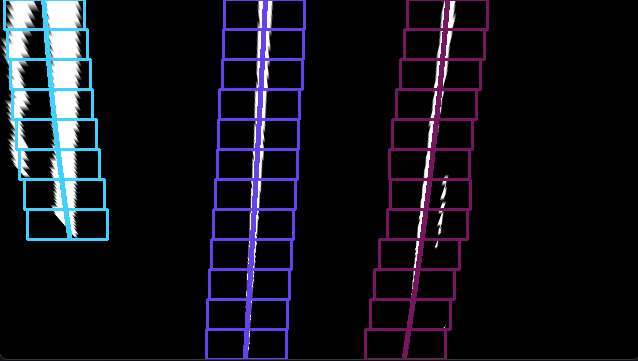
\includegraphics[width=7.5cm]{img/4_Implement/sliding_window/straight.png}
        \caption{Làn đường thẳng}
    \end{subfigure}%
    \begin{subfigure}{0.5\textwidth}
        \centering
        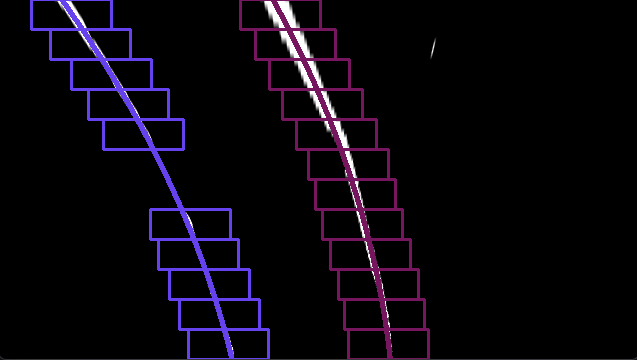
\includegraphics[width=7.5cm]{img/4_Implement/sliding_window/curve.png}
        \caption{Làn đường cong}
    \end{subfigure}
    \caption{Minh hoạ Curve Fitting trên làn đường}
\end{figure}\\
\textbf{Ưu điểm và nhược điểm}
\subsubsection{Phân tích, tổng hợp các phương pháp}
\newpage
\subsection{Lane Tracking}
\begin{itemize}
    \item \textbf{Input:} Phương trình các làn đường
    \item \textbf{Output:} Độ lệch của robot
\end{itemize}
\subsubsection{Xác định làn đường trái, phải}
Sau khi có tập hợp các đường thẳng, ta sẽ sắp xếp chúng theo độ lệch và xác định làn trái và phải gần nhất với robot. Độ lệch của làn đường sẽ được tính bằng tổng của toạ độ x của mỗi điểm trên làn đường và chia cho chiều cao của ảnh:
\begin{equation}
    d = \frac{w}{2} - \frac{\sum_{y = 0}^{h}x(y)}{h}
\end{equation}
Trong đó,
\begin{itemize}
    \item w, h: Kích thước của ảnh
    \item x = x(y), y: Toạ độ của một điểm trên phương trình làn đường
    \item d: Làn đường sẽ nằm bên trái nếu độ lệch nhỏ hơn 0 và ngược lại, làn đường sẽ nằm bên phải
\end{itemize}
\begin{figure}[!hbt]
\begin{center}
    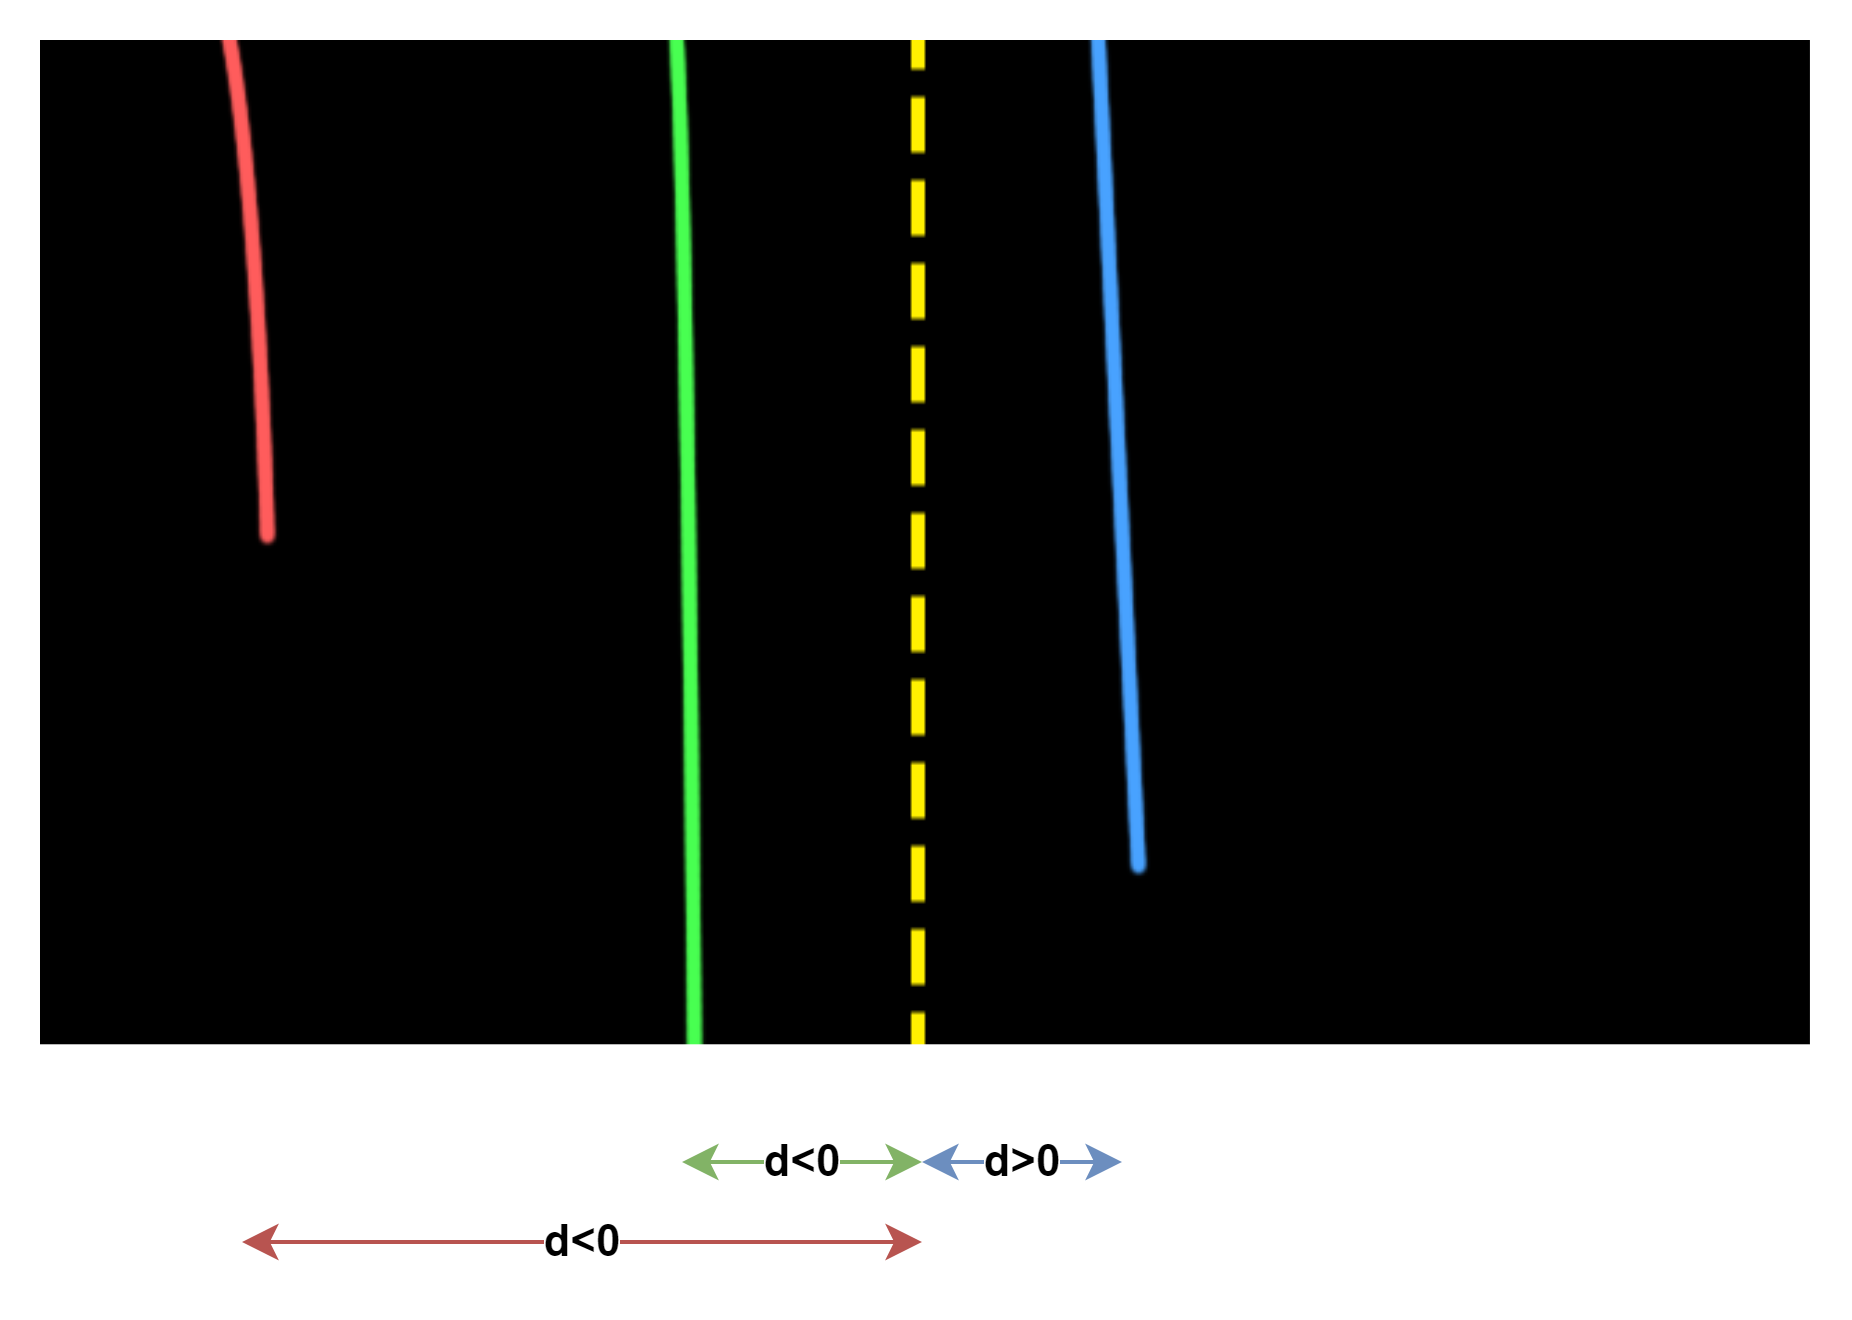
\includegraphics[width=13cm]{img/4_Implement/lane_tracking/lane_distance.png}
    \caption{Minh hoạ độ lệch các làn đường}
\end{center}
\end{figure}
\subsubsection{Nội suy làn đường giữa dựa trên dữ kiện làn đường trái, phải}
Để tìm được độ lệch của robot thì ta chỉ cần xác định được làn đường giữa và độ lệch robot chính là độ lệch của làn đường giữa. Dựa vào dữ kiện hai làn đường trước đó, ta sẽ nội suy được làn đường giữa trong các trường hợp sau:\\\\
\textbf{Có đủ dữ kiện cả 2 làn:} Phương trình làn đường giữa sẽ được tính bằng:
\begin{equation}
    x = \frac{a_L + a_R}{2}y^2 + \frac{b_L + b_R}{2}y + \frac{c_L + c_R}{2}
\end{equation}
Trong đó,
\begin{itemize}
    \item $a_L, b_L, c_L$: Hệ số phương trình làn đường trái
    \item $a_R, b_R, c_R$: Hệ số phương trình làn đường phải
\end{itemize}
\textbf{Chỉ có dữ kiện của 1 làn}: Bởi vì việc phân đoạn làn đường của mô hình AI có diễn ra sai sót, hoặc không đủ mạnh để có thể có được hoàn toàn hai làn đường, mà chỉ phát hiện được một làn đường (do có vật thể chắn, hoặc góc xoay camera dẫn đến khuất mạnh phần đường còn lại, ...). Việc dựa trên làn đường ở frame trước sẽ dẫn đến sai sót khi view camera thay đổi nhiều. Để xác định làn đường còn lại, nhóm sử dụng dữ kiện từ một làn đường hiện tại và ánh xạ song song với khoảng cách giữa hai làn đường đã biết. Cụ thể:
\begin{itemize}
    \item Cho một làn đường biết trước $L = L_i$ với $i \in \{L, R\}$
    \item Cho $d$ là khoảng cách giữa hai làn đường đã biết trước
    \item $\beta$ là làn đường cần tìm, $\beta \in \{L_L, L_R\}$. Nếu ta đã biết trước làn đường trái $L = L_L$ thì $\beta = L_R$ và ngược lại
    \item Với mỗi điểm $P(x, y)$ thuộc làn đường $L$, ta sẽ có điểm $P' = 
    \begin{cases}
        P'(x + d, y) & \text{nếu } \beta = L_R \\
        P'(x - d, y) & \text{nếu } \beta = L_L
    \end{cases}$
    là điểm thuộc làn đường $\beta$
    \item Sau khi có tập hợp các điểm $P'$ thì ta sẽ nội suy được phương trình làn đường $\beta$
\end{itemize}
\newpage
\section{Module bám làn đường}
Module bám làn đường sử dụng độ lệch làn đường $d$, là giá trị đầu ra của mô hình nhận diện làn đường, để thực hiện tính toán tốc độ góc thông qua thuật toán PID\textsuperscript{\cite{pid}}. Sau đó module sẽ gửi message Twist để điều khiển robot. Thành phần angular\_z trong Twist được dùng để xoay robot. Nhiệm vụ đặt ra là điều khiển angular\_z để xoay điểm chính giữa A của camera đến đúng vị trí O với các yêu cầu: chính xác (accurate), nhanh (fast response) và ổn định (small overshot).\\
\begin{figure}[!hbt]
    \begin{subfigure}{0.4\textwidth}
        \centering
        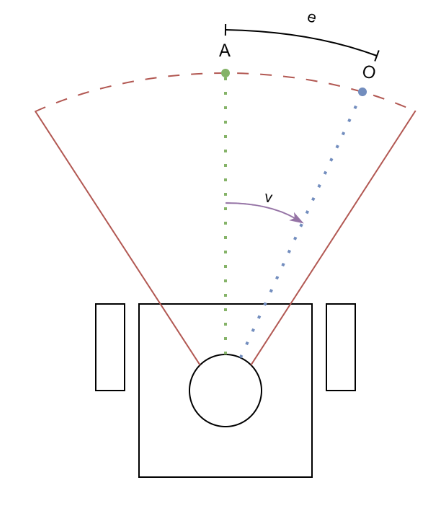
\includegraphics[width=6.5cm]{img/4_Implement/lane_keeping/top_down_view.png}
        \caption{Góc nhìn từ trên xuống}
    \end{subfigure}%
    \begin{subfigure}{0.6\textwidth}
        \centering
        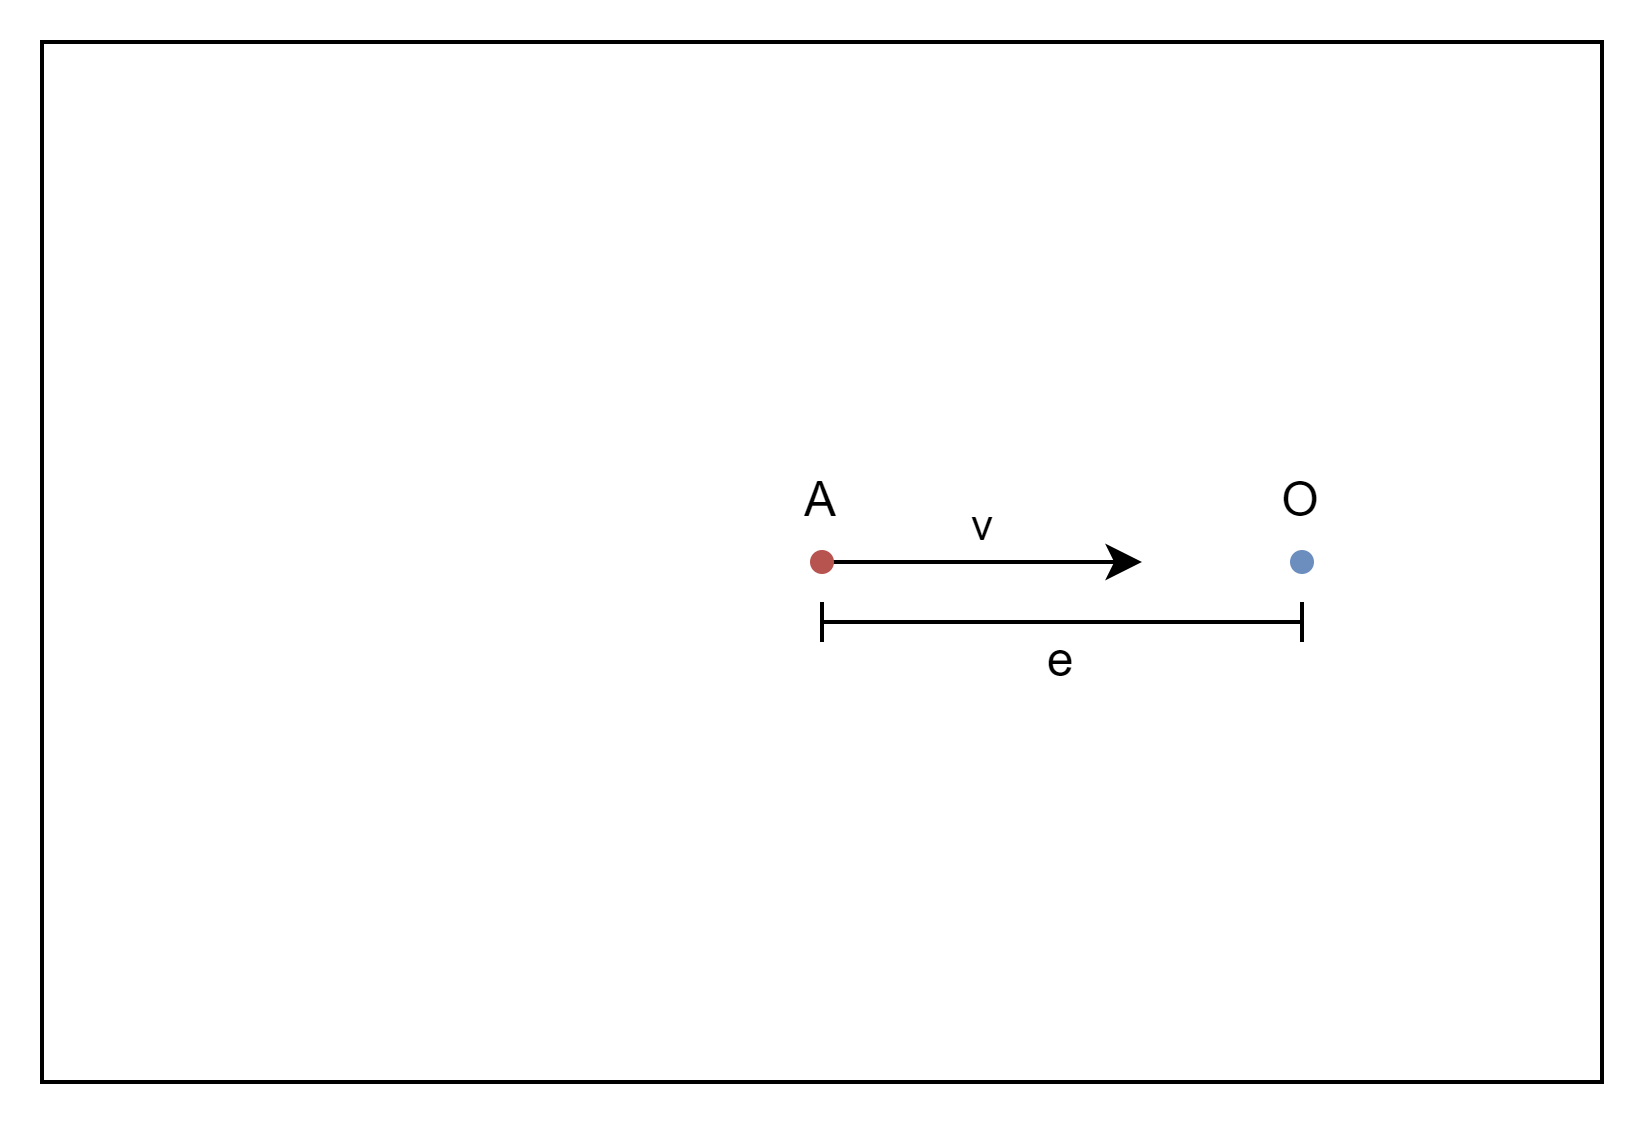
\includegraphics[width=8.5cm]{img/4_Implement/lane_keeping/camera_view.png}
        \caption{Góc nhìn camera}
    \end{subfigure}
    \caption{Minh họa điều khiển robot}
\end{figure}\\
\noindent Một điều rất tự nhiên, nếu vị trí hiện tại (điểm A) rất xa với vị trí mong muốn (điểm O), hay nói cách khác là sai số (error) lớn, ta cần điều chỉnh tốc độ xoay lớn để nhanh chóng đưa robot xoay đến vị trí O. Một cách đơn giản để công thức hoá lý tưởng này là dùng quan hệ tuyến tính:
\begin{equation}
    v = K_pe
\end{equation}
Trong đó $K_p$ là một hằng số dương mà ta gọi là hệ số P (Proportional Gain), $e$ là sai số cần điều khiển tức là khoảng cách từ điểm A tới điểm O. Mục tiêu điều khiển là đưa e tiến về 0 càng nhanh càng tốt. Rõ ràng nếu $K_p$ lớn thì $v$ cũng sẽ rất lớn và robot sẽ nhanh chóng xoay về vị trí O. Tuy nhiên khi đã đến vị trí O (tức $e = 0$), thì tuy vận tốc $v = 0$ nhưng do quán tính, robot vẫn tiếp tục xoay về bên phải và lệch điểm O về bên phải, sai số $e$ lại trở nên khác 0, giá trị sai số lúc này gọi là overshot (vượt quá). Lúc này, sai số $e < 0$, vận tốc $v$ sẽ xuất hiện với chiều ngược lại để kéo robot về điểm O. Nhưng một lần nữa, do $K_p$ lớn nên giá trị vận tốc $v$ cũng lớn và có thể kéo robot lệch về bên trái điểm O. Quá trính cứ tiếp diễn, robot cứ mãi dao động nhỏ dần quanh điểm O. Bộ điều khiển lúc này được nói là không ổn định.\\

\noindent Nhằm giảm overshot của robot, ta sẽ sử dụng một thành phần "thắng" trong bộ điều khiển. Sẽ rất lý tưởng nếu robot đang ở xa điểm O. Bộ điều sinh ra vận tốc $v$ lớn nhưng khi đã tiến gần đến điểm O thì thành phần "thắng" sẽ giảm tốc độ xoay của robot lại. Thành phần "thắng" này chính là thành phần D (Derivative), ta sẽ thu được bộ điều khiển PD như sau:
\begin{equation}
    v = K_pe + K_d\frac{de}{dt}
\end{equation}
Trong đó $\frac{de}{dt}$ là vận tốc thay đổi của sai số $e$ và $K_d$ là một hằng số dương gọi là hệ số D (Derivative Gain). Truy nhiên, trong đồ án này nhóm sẽ lược bớt thành phần I (Integral Gain), bộ điều khiển bây giờ sẽ là bộ điều khiển PD.\\

\noindent Có rất nhiều cách để chọn được thông số $K_p$ và $K_d$, nhóm sẽ chọn một cách thủ công bắt đầu từ $K_p = K_d = 0$, $K_p$ được tăng dần cho đến khi sai số $e$ bắt đầu dao động thì tăng $K_d$. Tại thời điểm $t = 0$, vị trí robot được thiết lập lệch khỏi làn đường là 80 ($e = 80$). Sau đó nhóm sẽ quan sát sự thay đổi của $e$ và đánh giá sự nhanh chóng, ổn định của bộ điều khiển.
\newpage
\begin{figure}[!hbt]
\begin{center}
    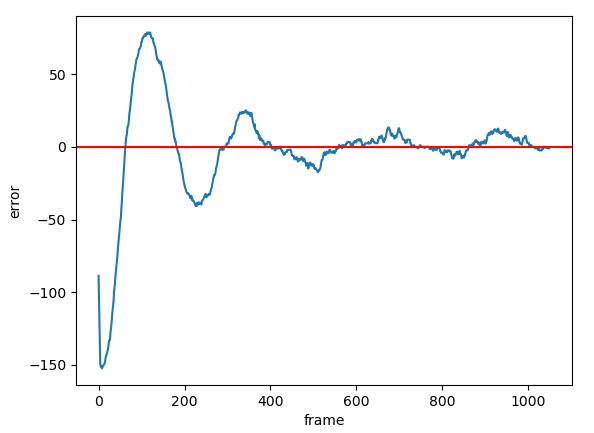
\includegraphics[width=12cm]{img/4_Implement/lane_keeping/error_plot.png}
    \caption{\label{pid_error_plot} Đồ thị sai số theo thời gian với $K_p = 0.0025, K_d = 0.007$}
\end{center}
\end{figure}
\noindent Có thể thấy ở hình \ref{pid_error_plot} có hiện tượng giống như overshoot, nhưng thực tế không phải là vậy. Nguyên nhân của hiện tượng này là do hiện tại robot đang được điều khiển thông qua tốc độ góc (angular\_z). Mặc dù tốc độ góc đang ở giá trị bằng 0, nhưng góc của robot vẫn có thể khác 0. Do robot luôn di chuyển theo hướng phía trước, khi góc của nó khác 0, robot sẽ đi chệch khỏi làn đường.
\begin{figure}[!hbt]
    \centering
    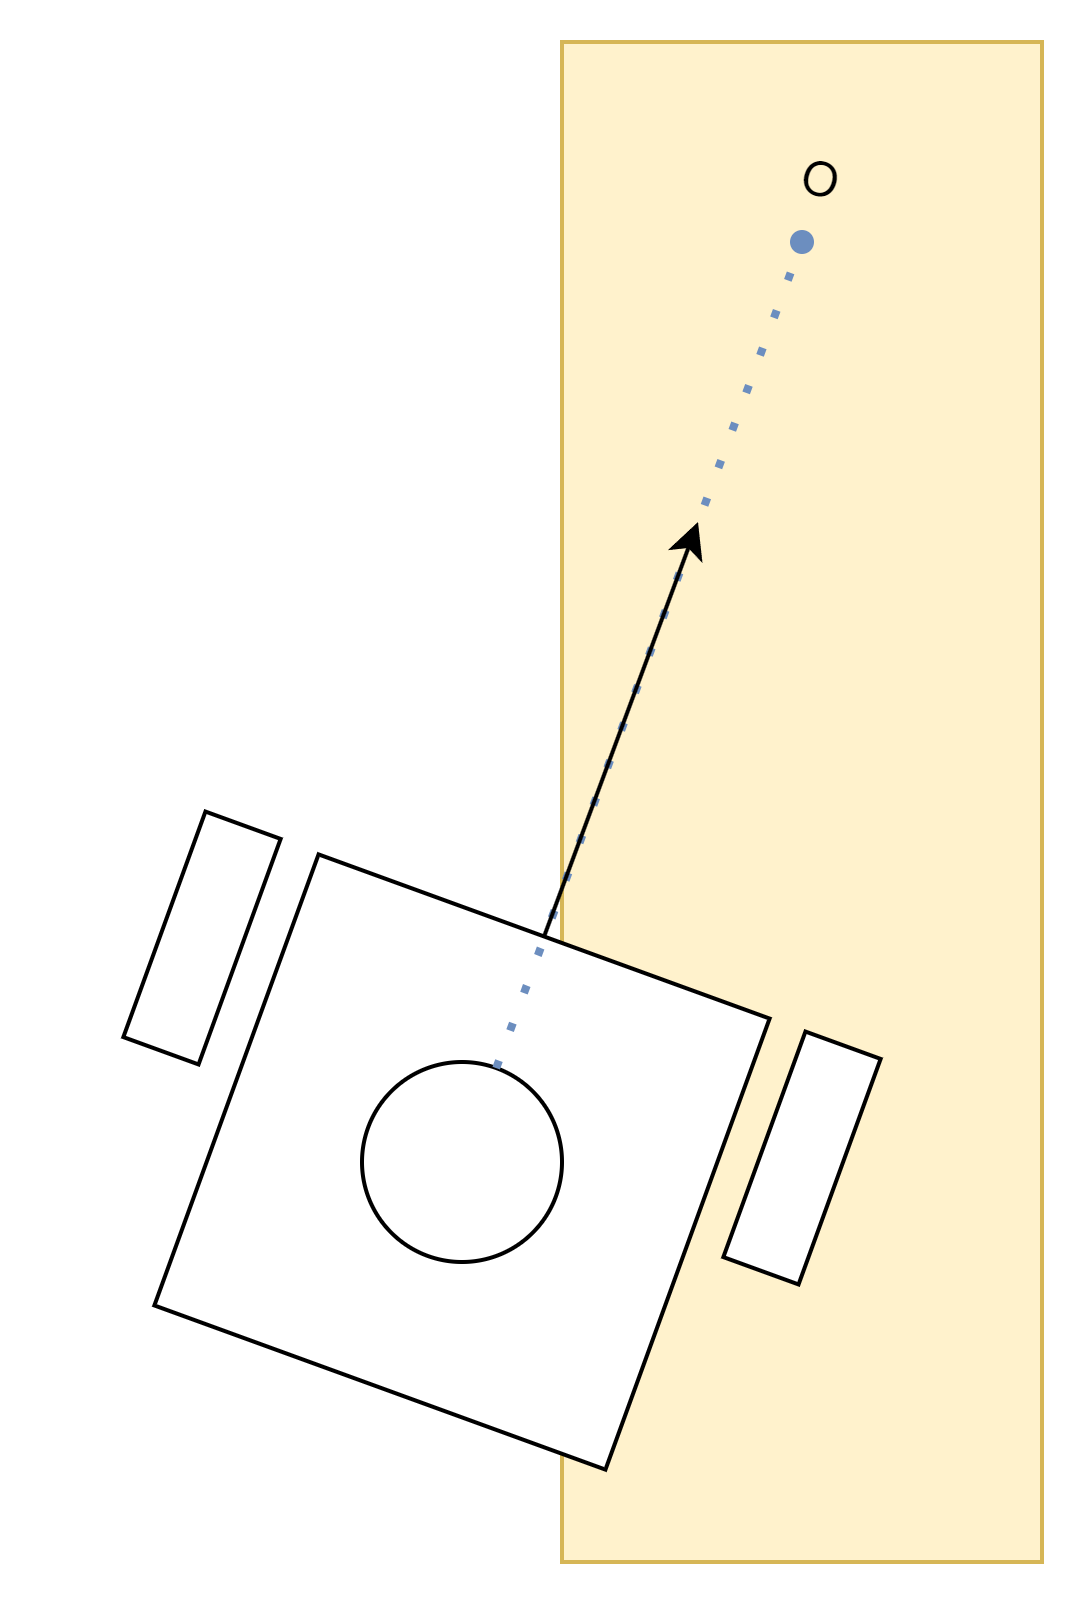
\includegraphics[width=5.5cm]{img/4_Implement/lane_keeping/error_view.png}
    \caption{Minh hoạ trường hợp đi lệch của robot}
\end{figure}
\newpage
\include{src/5_Result}
\newpage
% \chapter{Khó khăn gặp phải}
\newpage
% \chapter{Hướng phát triển}
\newpage
\chapter{Kết luận}
\section{Kết quả đạt được}
\begin{figure}[!hbt]
\begin{center}
    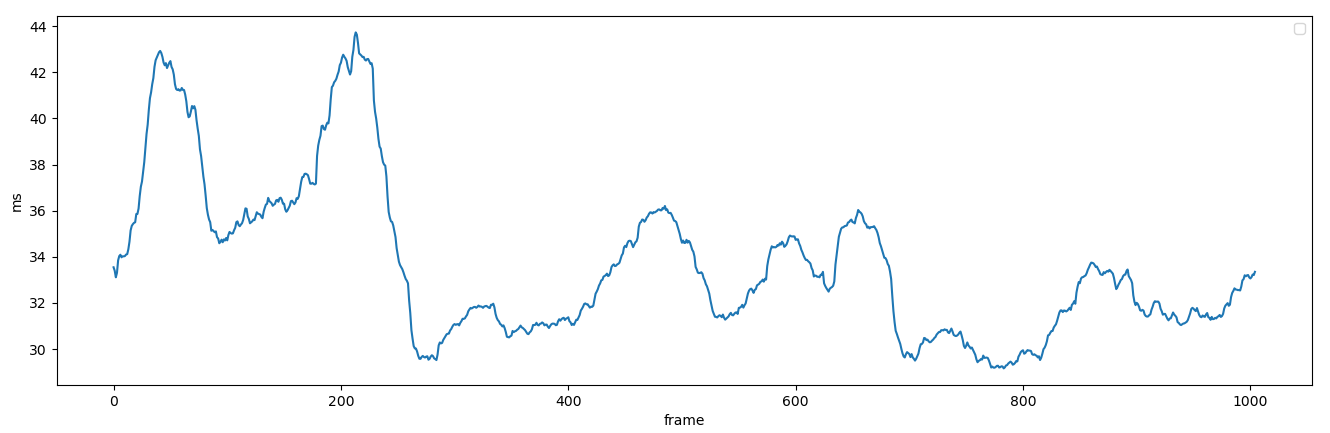
\includegraphics[width=16cm]{img/5_Conclusion/performane_plot_2.png}
    \caption{Thời gian thực thi của hệ thống}
\end{center}
\end{figure}
\begin{itemize}
    \item Trong biểu đồ trên, đường màu cam đại diện cho model AI và xanh đại diện cho khối backend. Ta dễ thấy thời gian xử lý tối thiểu cho 1 frame không quá 30ms nếu frame đó không là frame chứa lỗi/nhiễu. Tuy nhiên, nếu frame đó là frame lỗi, thời gian thực thi có thể lên đến 40ms cho 1 frame. Nhóm sẽ nghiên cứu cải thiện để tìm ra cách tối ưu nhất để cho ra kết quả tối ưu cuối cùng.
    \item Robot có khả năng tuân thủ làn đường, di chuyển với tốc độ trung bình mà không lệch hướng.
    \item Bộ điều khiển PID của hệ thống đã duy trì vị trí chính xác và ổn định trên làn đường
    \item Khi phát hiện có nguy cơ lệch khỏi làn đường, hệ thống sẽ kịp thời đưa ra cảnh báo nguy cơ lệch khỏi làn đường.
    
\end{itemize}
\section{Khó khăn gặp phải}
Có thể thấy, dù hệ thống hoạt động tương đối tốt, robot có khả năng chạy đủ ổn định để hoàn thành kịch bản demo và đạt được mục tiêu đề ra, tuy nhiên vẫn còn một số vấn đề còn tồn đọng như sau:
\begin{enumerate}
    \item \textbf{Khối nhận diện làn đường:}
    \begin{itemize}
        \item 
        \item 
    \end{itemize}
    \item \textbf{Khối bám làn đường:} Module hiện tại chỉ dựa vào chỉ một thông số độ lệch làn đường duy nhất và vẫn chưa ổn định vì cũng chỉ điều khiển mỗi tốc độ góc của TurtleBot3
\end{enumerate}

\bibliographystyle{ieeetr}
\bibliography{refs.bib}
\end{document}